\documentclass[12pt]{article}

\usepackage[indonesian]{babel}
\usepackage[a4paper, top=2.5cm, bottom=2.5cm, left=3cm, right=2.5cm,
            headheight=1.6cm, headsep=0.4cm]{geometry}

% Font Times 
\usepackage{mathptmx}

% Paket
\usepackage{amsmath}
\usepackage{amssymb}
\usepackage{graphicx}
\usepackage[colorlinks=true, allcolors=black, urlcolor=blue]{hyperref}
\usepackage{fancyhdr}
\usepackage{lastpage}
\usepackage{listings}
\usepackage{xcolor}
\usepackage{array}
\usepackage{float}
\usepackage{booktabs}
\usepackage{placeins}

% METADATA
\newcommand{\kodematkul}{IF2123}
\newcommand{\namamatkul}{Aljabar Linier dan Geometri}
\newcommand{\judullaporan}{Laporan Tugas Besar 1}
\newcommand{\subjudul}{Sistem Persamaan Linier, Determinan, dan Penerapannya}
\newcommand{\semester}{Semester I Tahun 2026/2027}
\newcommand{\namakelompok}{sukses lancar berkah}
\newcommand{\nomorkelompok}{38}
\newcommand{\linkgithub}{https://github.com/nuha-alghifari/algeo26-tb1-sukses-lancar-berkah}
\newcommand{\linkvideo}{https://youtu.be/xxxxxxxxxxx}

% Anggota kelompok
\newif\ifempat
\empatfalse
\newcommand{\anggotaa}{Ahmad Humam Isma}
\newcommand{\nima}{13525032}
\newcommand{\anggotab}{Mochammad Nuha Al Ghifari}
\newcommand{\nimb}{13525056}
\newcommand{\anggotac}{Athallah Nanda Andita}
\newcommand{\nimc}{13525148}

% Saklar bonus
\newif\ifbonusgui         \bonusguifalse
\newif\ifbonusinpainting  \bonusinpaintingfalse
\newif\ifbonusvideo       \bonusvideofalse
\newif\ifbonuslatex       \bonuslatextrue

% Placeholder gambar
% Ganti dengan \includegraphics{...} kalau berkasnya sudah ada.
\newcommand{\gambarplaceholder}[2][0.5\linewidth]{%
    \fbox{\parbox[c][3cm][c]{#1}{\centering \textit{#2}}}}

% Gaya blok keluaran program
\definecolor{backcolour}{rgb}{0.95,0.95,0.92}
\lstdefinestyle{keluaranstyle}{
    backgroundcolor=\color{backcolour},
    basicstyle=\footnotesize\ttfamily,
    breaklines=true,
    breakatwhitespace=false,
    keepspaces=true,
    numbers=none,
    showspaces=false,
    showstringspaces=false,
    showtabs=false,
    tabsize=2,
    columns=fullflexible,
    frame=single,
    framerule=0.2pt,
    rulecolor=\color{black!30},
    xleftmargin=0pt,
    aboveskip=0.6em,
    belowskip=0.6em
}
\lstnewenvironment{keluaran}{\lstset{style=keluaranstyle}}{}

\newcommand{\kasusuji}[1]{%
    \subsubsection{Kasus Uji #1}
    \paragraph{Input.} Tuliskan matriks/data masukan yang diberikan.
    \[
        \begin{bmatrix} \cdots & \cdots \\ \cdots & \cdots \end{bmatrix}
    \]
    \paragraph{Output.} Hasil yang dihasilkan program:
}
\newcommand{\analisis}{%
    \paragraph{Analisis.} Apakah hasil sesuai solusi eksak? Bagaimana perbandingan
    antarmetode (jika berbeda, jelaskan penyebabnya, misalnya galat pembulatan)?
}

% Header & footer
\pagestyle{fancy}
\fancyhf{}
\renewcommand{\headrulewidth}{0.4pt}
\renewcommand{\footrulewidth}{0.4pt}
\renewcommand{\contentsname}{Daftar Isi}
\renewcommand{\tablename}{Tabel}
\renewcommand{\figurename}{Gambar}


\rhead{
    \begin{tabular}{@{}r@{}}
        \footnotesize \kodematkul{} \namamatkul \\
        \footnotesize \judullaporan \\
        \footnotesize \semester
    \end{tabular}
}
\lfoot{\small Kelompok \nomorkelompok{} -- \namakelompok}
\rfoot{\small Halaman \thepage \ dari \pageref{LastPage}}

\begin{document}

% COVER: judul, kode & nama matkul, nama+NIM anggota, foto bersama
\begin{titlepage}
    \thispagestyle{fancy}
    \centering

    {\huge \bfseries \judullaporan \par}
    \vspace{1em}
    {\Large \kodematkul{} \MakeUppercase{\namamatkul} \par}
    \vspace{0.5em}
    {\large \MakeUppercase{\subjudul} \par}
    \vspace{0.5em}
    {\large \MakeUppercase{\semester} \par}

    \vspace{1.5em}
    
\includegraphics[width=0.8\textwidth]{imgs/foto kelompok.png}

    \vspace{1.5em}
    {\large Kelompok \nomorkelompok{} -- \namakelompok \par}
    \vspace{0.5em}
    \begin{tabular}{l l}
        \anggotaa & \nima \\
        \anggotab & \nimb \\
        \anggotac & \nimc \\
        \ifempat \anggotad & \nimd \\ \fi
    \end{tabular}

    \vfill
    

    {\large LABORATORIUM ILMU DAN REKAYASA KOMPUTASI \par}
    \vspace{0.3em}
    PROGRAM STUDI TEKNIK INFORMATIKA \par
    \vspace{0.3em}
    SEKOLAH TEKNIK ELEKTRO DAN INFORMATIKA \par
    \vspace{0.3em}
    INSTITUT TEKNOLOGI BANDUNG \par
\end{titlepage}

\tableofcontents

% BAB 1 -- PENDAHULUAN
\newpage
\section{Pendahuluan}
\subsection{Deskripsi Masalah}
Tugas besar ini menuntut pengembangan sebuah pustaka aljabar linier dan geometri secara mandiri menggunakan bahasa pemrograman Java, tanpa bergantung pada pustaka matematika atau pustaka numerik eksternal. Perangkat lunak yang dibangun harus mampu merepresentasikan struktur data matriks secara komputasional dan menjalankan berbagai metode numerik secara akurat, utamanya dengan memanfaatkan Operasi Baris Elementer (OBE).
\\

\noindent Permasalahan utama yang harus diselesaikan meliputi perancangan modul penyelesaian Sistem Persamaan Linier (Eliminasi Gauss, Gauss-Jordan, Matriks Balikan, dan Kaidah Cramer), perhitungan determinan dan invers matriks, serta penerapan aljabar linier pada persoalan aproksimasi fungsi, yaitu Interpolasi Polinomial, Interpolasi Natural Cubic Spline, dan Regresi Spline Kubik. Program juga harus diintegrasikan ke dalam antarmuka baris perintah (Command Line Interface) yang interaktif, dilengkapi dengan sistem penanganan galat masukan (exception handling), dan memiliki kemampuan membaca serta menyimpan data matriks melalui interaksi operasi berkas berekstensi .txt.

\subsection{Latar Belakang}
Aljabar linier merupakan salah satu fondasi matematis yang paling esensial dalam bidang komputasi modern. Konsep-konsep seperti vektor, matriks, dan transformasi linier menjadi landasan utama bagi berbagai disiplin ilmu komputer tingkat lanjut, termasuk pemrosesan citra digital, grafika komputer, hingga pembelajaran mesin (machine learning). Banyak permasalahan kompleks di dunia nyata yang dapat disederhanakan dan diselesaikan secara algoritmik apabila dimodelkan ke dalam bentuk Sistem Persamaan Linier (SPL).
\\

\noindent Meskipun saat ini pengembang perangkat lunak sangat dimanjakan dengan ketersediaan berbagai pustaka numerik instan yang teroptimasi, penggunaan pustaka tersebut sering kali menjadikan algoritma perhitungan sebagai sebuah "kotak hitam" (black box). Ketergantungan ini berpotensi mereduksi pemahaman fundamental mengenai logika komputasi di balik penyelesaian matriks, seperti masalah stabilitas numerik, pivoting, dan kompleksitas waktu.
\\

\noindent Oleh karena itu, pembangunan sebuah pustaka aljabar linier dari dasar (from scratch) menjadi proses pembelajaran yang krusial. Selain melatih kemampuan rekayasa perangkat lunak dalam menyusun arsitektur program modular dan abstraksi struktur data, kegiatan ini bertujuan memberikan pemahaman mendalam mengenai implementasi murni dari algoritma-algoritma numerik dasar. Dengan demikian, penerapan teori aljabar linier pada kasus aproksimasi fungsi dan manipulasi citra dapat dipahami logika perhitungannya secara utuh, bukan sekadar menggunakan fungsi siap pakai.

\subsection{Tujuan}
\begin{itemize}
    \item Mengimplementasikan metode penyelesaian SPL, determinan, invers matriks,           interpolasi polinomial, Natural Cubic Spline Interpolation, regresi Spline,        dan algoritma Image Inpainting berbasis diskritisasi Persamaan Laplace             secara mandiri menggunakan Java.
    \item Membangun pustaka (library) aljabar linier yang terstruktur secara modular,        bersih, dan terdokumentasi dengan baik. Tidak menggunakan library                  perhitungan matriks, regresi, atau interpolasi instan.
    \item Menguji keandalan pustaka pada berbagai kasus uji analitis dan restorasi           citra, serta menyusun laporan analisis hasil perhitungannya.
\end{itemize}

% BAB 2 -- DASAR TEORI
\section{Dasar Teori}

\subsection{Sistem Persamaan Linier}
Sistem Persamaan Linier (SPL) adalah himpunan berhingga dari $m$ buah persamaan linier dengan $n$ buah variabel riil $x_1, x_2, \dots, x_n$. Bentuk umum SPL dinotasikan sebagai:
\begin{equation}
    \begin{cases}
        a_{11}x_1 + a_{12}x_2 + \dots + a_{1n}x_n = b_1 \\
        a_{21}x_1 + a_{22}x_2 + \dots + a_{2n}x_n = b_2 \\
        \vdots \\
        a_{m1}x_1 + a_{m2}x_2 + \dots + a_{mn}x_n = b_m
    \end{cases}
\end{equation}
SPL tersebut dapat direpresentasikan secara ringkas ke dalam bentuk persamaan matriks 
$\mathbf{A}\mathbf{x} = \mathbf{b}$, di mana $\mathbf{A} \in \mathbb{R}^{m \times n}$ adalah matriks koefisien, $\mathbf{x} \in \mathbb{R}^{n \times 1}$ adalah vektor variabel, dan $\mathbf{b} \in \mathbb{R}^{m \times 1}$ adalah vektor konstanta. Gabungan matriks koefisien dan vektor konstanta membentuk matriks augmented $[\mathbf{A} \mid \mathbf{b}]$:

Berdasarkan solusinya, SPL dibagi menjadi tiga jenis yaitu:
\begin{enumerate}
    \item \textbf{Solusi Tunggal:} Terjadi jika setiap baris matriks augmented yang telah dilakukan OBE memiliki satu utama sehingga menjadi bentuk matriks eselon baris/eselon baris tereduksi.
    \begin{equation}
    M = 
    \begin{bmatrix}
        1 & 1 & 1 & \mid & 0 \\
        0 & 1 & -1 & \mid & 1 \\
        0 & 0 & 1 & \mid & 1 \\
    \end{bmatrix}
    \end{equation}
    \item \textbf{Solusi Banyak/Tak Terhingga} Terjadi jika matriks augmented yang telah dilakukan operasi OBE memiliki baris terakhir yang seluruhnya bernilai 0.
    \begin{equation}
    M = 
    \begin{bmatrix}
        1 & 1 & 2 & \mid & 4 \\
        0 & 1 & 1 & \mid & 2 \\
        0 & 0 & 0 & \mid & 0 \\
    \end{bmatrix}
    \end{equation}
    \item \textbf{Tidak Ada Solusi } Terjadi jika matriks augmented yang telah dilakukan operasi OBE memiliki baris terakhir bernilai 0 kecuali pada kolom terakhir.
    \begin{equation}
    M = 
    \begin{bmatrix}
        1 & 1 & 2 & \mid & 4 \\
        0 & 1 & 1 & \mid & 2 \\
        0 & 0 & 0 & \mid & 1 \\
    \end{bmatrix}
    \end{equation}

\subsubsection{Eliminasi Gauss}
Metode Eliminasi Gauss mereduksi matriks augmented $[\mathbf{A} \mid \mathbf{b}]$ menjadi bentuk Matriks Eselon Baris menggunakan Operasi Baris Elemen (OBE). Setelah bentuk eselon baris terbentuk, nilai setiap variabel diperoleh melalui teknik \textit{substitusi mundur}

\subsubsection{Eliminasi Gauss-Jordan}
Eliminasi Gauss-Jordan merupakan perluasan dari Eliminasi Gauss dengan melanjutkan proses OBE hingga matriks mencapai bentuk Matriks Eselon Baris Tereduksi. Seluruh elemen di atas dan di bawah pivot $1$ dinolkan. Solusi SPL dapat dibaca secara langsung dari kolom terakhir matriks tanpa memerlukan substitusi mundur.

\subsubsection{Metode Matriks Balikan}
Jika matriks $\mathbf{A}$ merupakan matriks persegi ($n \times n$) dan nonsingular ($\det(\mathbf{A}) \neq 0$), maka matriks memiliki invers $\mathbf{A}^{-1}$. Solusi SPL dapat dihitung secara langsung melalui perkalian matriks:
\begin{equation}
    \mathbf{x} = \mathbf{A}^{-1}\mathbf{b}
\end{equation}

\subsubsection{Kaidah Cramer}
Kaidah Cramer berlaku untuk SPL persegi ($n \times n$) dengan syarat matriks koefisien nonsingular ($\det(\mathbf{A}) \neq 0$). Nilai variabel $x_j$ dihitung menggunakan perbandingan determinan:
\begin{equation}
    x_j = \frac{\det(\mathbf{A}_j)}{\det(\mathbf{A})}, \quad j = 1, 2, \dots, n
\end{equation}
di mana $\mathbf{A}_j$ adalah matriks yang diperoleh dengan mengganti kolom ke-$j$ pada matriks $\mathbf{A}$ dengan vektor konstanta $\mathbf{b}$.

\subsection{Determinan Matriks}
Determinan adalah skalar khusus yang diasosiasikan dengan matriks persegi $\mathbf{A} \in \mathbb{R}^{n \times n}$, dinotasikan dengan $\det(\mathbf{A})$ atau $|\mathbf{A}|$.

\subsubsection{Reduksi Baris (OBE)}
Penyelesaian determinan menggunakan OBE memanfaatkan sifat-sifat matriks segitiga atas $\mathbf{U}$, di mana determinan adalah hasil kali elemen diagonal utamanya. Pengaruh OBE terhadap determinan matriks adalah:
\begin{itemize}
    \item Pertukaran dua baris ($R_i \leftrightarrow R_j$) mengubah tanda determinan: $\det(\mathbf{A}') = -\det(\mathbf{A})$.
    \item Perkalian satu baris dengan skalar $k$ ($R_i \leftarrow k R_i$) mengalikan determinan: $\det(\mathbf{A}') = k \cdot \det(\mathbf{A})$.
    \item Penambahan kelipatan suatu baris ke baris lain ($R_i \leftarrow R_i + k R_j$) tidak mengubah nilai determinan.
\end{itemize}
Maka, determinan matriks dapat dihitung melalui:
\begin{equation}
    \det(\mathbf{A}) = (-1)^s \prod_{i=1}^{n} u_{ii}
\end{equation}
di mana $s$ adalah jumlah pertukaran baris yang dilakukan.

\subsubsection{Ekspansi Kofaktor}
Metode ekspansi kofaktor menghitung determinan dengan memetakan matriks ke dalam submatriks berukuran lebih kecil. Kofaktor $C_{ij}$ dari elemen $a_{ij}$ didefinisikan sebagai:
\begin{equation}
    C_{ij} = (-1)^{i+j} M_{ij}
\end{equation}
di mana $M_{ij}$ adalah minor elemen $a_{ij}$ (determinan submatriks $(n-1)\times(n-1)$ setelah menghapus baris ke-$i$ dan kolom ke-$j$). Ekspansi sepanjang baris ke-$i$ dirumuskan sebagai:
\begin{equation}
    \det(\mathbf{A}) = \sum_{j=1}^{n} a_{ij} C_{ij}
\end{equation}

\subsection{Matriks Balikan (Invers)}
Suatu matriks persegi $\mathbf{A}$ memiliki invers $\mathbf{A}^{-1}$ jika dan hanya jika $\mathbf{A}$ nonsingular ($\det(\mathbf{A}) \neq 0$), sedemikian hingga $\mathbf{A}\mathbf{A}^{-1} = \mathbf{A}^{-1}\mathbf{A} = \mathbf{I}_n$.

\subsubsection{Metode Augmentasi}
Metode ini menggunakan Eliminasi Gauss-Jordan pada matriks teraugmentasi yang menggabungkan matriks $\mathbf{A}$ dengan matriks identitas $\mathbf{I}_n$:
\begin{equation}
    [\mathbf{A} \mid \mathbf{I}_n] \xrightarrow{\text{OBE}} [\mathbf{I}_n \mid \mathbf{A}^{-1}]
\end{equation}
Jika matriks $\mathbf{A}$ tidak dapat direduksi menjadi $\mathbf{I}_n$, maka $\mathbf{A}$ bersifat singular (tidak memiliki invers).

\subsubsection{Metode Adjoin}
Invers matriks dapat ditentukan menggunakan matriks kofaktor dan adjoin, yang dirumuskan sebagai:
\begin{equation}
    \mathbf{A}^{-1} = \frac{1}{\det(\mathbf{A})} \operatorname{adj}(\mathbf{A})
\end{equation}
di mana $\operatorname{adj}(\mathbf{A}) = \mathbf{C}^T$ adalah transpose dari matriks kofaktor $\mathbf{C} = [C_{ij}]$.

\subsection{Interpolasi Polinomial}
Diberikan $n+1$ titik data sampel yang saling berbeda $(x_0, y_0), (x_1, y_1), \dots, (x_n, y_n)$. Interpolasi polinomial bertujuan menentukan polinom $P_n(x)$ derajat berorde paling tinggi $n$:
\begin{equation}
    P_n(x) = a_0 + a_1 x + a_2 x^2 + \dots + a_n x^n
\end{equation}
yang memenuhi $P_n(x_i) = y_i$ untuk setiap $i = 0, 1, \dots, n$. Substitusi seluruh titik data menghasilkan Sistem Persamaan Linier dengan Matriks Vandermonde:
\begin{equation}
    \begin{bmatrix}
        1 & x_0 & x_0^2 & \dots & x_0^n \\
        1 & x_1 & x_1^2 & \dots & x_1^n \\
        \vdots & \vdots & \vdots & \ddots & \vdots \\
        1 & x_n & x_n^2 & \dots & x_n^n
    \end{bmatrix}
    \begin{bmatrix} a_0 \\ a_1 \\ \vdots \\ a_n \end{bmatrix}
    =
    \begin{bmatrix} y_0 \\ y_1 \\ \vdots \\ y_n \end{bmatrix}
\end{equation}
Koefisien polinomial $a_0, a_1, \dots, a_n$ diperoleh dengan menyelesaikan SPL Vandermonde tersebut menggunakan Eliminasi Gauss.

\subsection{Natural Cubic Spline Interpolation}
Interpolasi Spline Kubik mengonstruksi kurva mulus berupa potongan-potongan polinom berderajat tiga $S_j(x)$ pada setiap sub-interval $[x_j, x_{j+1}]$ untuk $j = 0, 1, \dots, n-1$:
\begin{equation}
    S_j(x) = a_j + b_j(x - x_j) + c_j(x - x_j)^2 + d_j(x - x_j)^3
\end{equation}
Persyaratan kontinuitas turunan pertama dan kedua pada titik simpul interior (\textit{knot}) menghasilkan sistem persamaan berstruktur tridiagonal untuk menentukan turunan kedua $M_j = S''(x_j) = 2c_j$:
\begin{equation}
    h_{j-1} M_{j-1} + 2(h_{j-1} + h_j) M_j + h_j M_{j+1} = 6 \left( \frac{y_{j+1} - y_j}{h_j} - \frac{y_j - y_{j-1}}{h_{j-1}} \right)
\end{equation}
di mana $h_j = x_{j+1} - x_j$. Pada \textbf{Natural Cubic Spline}, diterapkan syarat batas alami pada kedua ujung domain:
\begin{equation}
    M_0 = M_n = 0
\end{equation}

\subsection{Regresi Spline Kubik}
Regresi Spline Kubik mengestimasi hubungan non-linier antara variabel prediktor $x$ dan respon $y$ menggunakan Truncated Power Basis dengan $K$ buah titik knot terdistribusi $\xi_1, \xi_2, \dots, \xi_K$. Fungsi regresi dimodelkan sebagai kombinasi linier dari $M = 4 + K$ fungsi basis:
\begin{equation}
    f(x) = \beta_0 + \beta_1 x + \beta_2 x^2 + \beta_3 x^3 + \sum_{k=1}^{K} \beta_{3+k} (x - \xi_k)_+^3
\end{equation}
di mana $(x - \xi_k)_+ = \max(0, x - \xi_k)$.

Diberikan $N$ titik data pengamatan, model disusun ke dalam bentuk persamaan matriks $\mathbf{y} = \mathbf{X}\boldsymbol{\beta} + \boldsymbol{\epsilon}$, di mana $\mathbf{X} \in \mathbb{R}^{N \times M}$ adalah matriks desain. Estimasi parameter koefisien $\hat{\boldsymbol{\beta}}$ diperoleh dengan meminimalkan jumlah kuadrat residu melalui Persamaan Normal:
\begin{equation}
    (\mathbf{X}^T\mathbf{X})\hat{\boldsymbol{\beta}} = \mathbf{X}^T\mathbf{y}
\end{equation}
Sehingga solusi koefisien regresi dirumuskan sebagai:
\begin{equation}
    \hat{\boldsymbol{\beta}} = (\mathbf{X}^T\mathbf{X})^{-1}\mathbf{X}^T\mathbf{y}
\end{equation}

\ifbonusinpainting
\subsection{Image Inpainting dengan Persamaan Laplace}
\textit{Image inpainting} bertujuan merekonstruksi piksel citra yang rusak/hilang pada domain $\Omega$ berdasarkan informasi piksel utuh pada batas wilayah $\partial\Omega$. Daerah yang hilang dimodelkan memenuhi Persamaan Laplace kontinu $\nabla^2 f = 0$.

Menggunakan pendekatan skema beda hingga pusat (*center finite difference*), diskritisasi Persamaan Laplace pada piksel $(i, j)$ dinyatakan sebagai rata-rata dari empat piksel tetangganya:
\begin{equation}
    f_{i,j} = \frac{f_{i+1,j} + f_{i-1,j} + f_{i,j+1} + f_{i,j-1}}{4}
\end{equation}
Formulasi ini membentuk Sistem Persamaan Linier berukuran besar $N \times N$ (di mana $N$ adalah jumlah piksel rusak). Untuk menyelesaikan SPL berukuran sangat besar tersebut secara efisien, digunakan metode iteratif **Jacobi** atau **Gauss-Seidel**. Skema pembaruan metode Gauss-Seidel pada iterasi ke-$(k+1)$ dirumuskan sebagai:
\begin{equation}
    f_{i,j}^{(k+1)} = \frac{f_{i-1,j}^{(k+1)} + f_{i+1,j}^{(k)} + f_{i,j-1}^{(k+1)} + f_{i,j+1}^{(k)}}{4}
\end{equation}
Proses iterasi dilanjutkan hingga mencapai kriteria konvergensi $\|f^{(k+1)} - f^{(k)}\| < \varepsilon$.
\fi

% BAB 3 -- IMPLEMENTASI
\section{Implementasi}
Penjelasan implementasi pustaka dan program dalam Java. Kode sumber tidak
dilampirkan di naskah; cukup dijelaskan strukturnya (kode ada di repositori
GitHub pada Lampiran).

\subsection{Struktur Kelas}
Tabel berikut merangkum struktur kelas-kelas penyusun pustaka matematika yang diimplementasikan pada tugas besar ini beserta atribut dan metode pentingnya.

\begin{table}[H]
    \centering
    \renewcommand{\arraystretch}{1.3}
    \begin{tabular}{|l|p{4cm}|p{6.5cm}|}
        \hline
        \textbf{Kelas} & \textbf{Atribut penting} & \textbf{Metode penting} \\
        \hline
        \texttt{Matriks} & \texttt{data}, \texttt{rows}, \texttt{cols} & \texttt{tambah()}, \texttt{kali()}, \texttt{tukarBaris()}, \texttt{kaliBaris()}, \texttt{tambahBaris()}, \texttt{printMatriks()} \\
        \hline
        \texttt{Determinan} & - & \texttt{reduksiBaris()}, \texttt{kofaktorRekursif()} \\
        \hline
        \texttt{SPL} & \texttt{EPS}, \texttt{EPS\_PIVOT} & \texttt{gauss()}, \texttt{gaussJordan()}, \texttt{eliminasiMaju()}, \texttt{eliminasiMundur()} \\
        \hline
        \texttt{HasilSPL} & \texttt{tipe}, \texttt{nilai}, \texttt{parametrik} & \texttt{tunggal()}, \texttt{tidakAda()}, \texttt{takHingga()}, \texttt{keTeks()} \\
        \hline
        \texttt{NaturalCubicSpline} & \texttt{x}, \texttt{a}, \texttt{b}, \texttt{c}, \texttt{d} & \texttt{hitungSpline()}, \texttt{evaluasiSpline()}, \texttt{printPersamaan()} \\
        \hline
        \texttt{CubicRegressionSpline} & \texttt{knots}, \texttt{beta} & \texttt{hitungRegresi()}, \texttt{prediksi()}, \texttt{printPersamaan()} \\
        \hline
    \end{tabular}
    \caption{Struktur kelas pada pustaka}
    \label{tab:kelas}
\end{table}

\subsection{Arsitektur Pustaka}
Pustaka aljabar linier ini dibangun dengan pendekatan modular, di mana kelas \texttt{Matriks} bertindak sebagai fondasi struktur data utama. Modul-modul lain memiliki ketergantungan (dependensi) terhadap kelas ini:
\begin{itemize}
    \item Modul \texttt{SPL} dan \texttt{Determinan} sangat bergantung pada metode-metode operasi baris dasar (OBE) yang disediakan oleh kelas \texttt{Matriks}.
    \item Modul \texttt{SPL} menghasilkan instansiasi dari kelas \texttt{HasilSPL} untuk membungkus nilai solusi secara rapi.
    \item Modul \texttt{NaturalCubicSpline} bekerja secara mandiri menggunakan array primitif dengan algoritma Thomas untuk efisiensi perhitungan sistem tridiagonal.
    \item Modul \texttt{CubicRegressionSpline} membangun matriks desain $\mathbf{X}$, lalu memanggil \texttt{SPL.gauss()} dari kelas terpisah untuk menyelesaikan sistem Persamaan Normal.
\end{itemize}

\subsection{Alur Program}
Program dieksekusi melalui antarmuka baris perintah (CLI) yang terpusat di kelas \texttt{App}. Alur program secara garis besar adalah sebagai berikut:
\begin{enumerate}
    \item \textbf{Menu Utama:} Program menampilkan pilihan menu modul algoritma (SPL, Determinan, Invers, Interpolasi, Regresi).
    \item \textbf{Pemilihan Input:} Pengguna memilih sumber masukan data (secara manual dari \textit{keyboard} atau membaca dari berkas \texttt{.txt}).
    \item \textbf{Penanganan Kesalahan (\textit{Exception Handling}):} Program diimplementasikan dengan blok \texttt{try-catch} untuk menangani masukan tidak valid (menghindari \texttt{Input\-Mismatch\-Exception}) atau masalah pembacaan berkas (\texttt{File\-Not\-Found\-Exception}) sehingga eksekusi tidak terhenti secara tiba-tiba.
    \item \textbf{Pemrosesan:} Data input dikonversi menjadi objek kelas \texttt{Matriks} dan diproses sesuai algoritma yang dipilih.
    \item \textbf{Output:} Hasil komputasi beserta langkah-langkah penyelesaiannya dicetak ke layar terminal melalui pemanggilan metode \texttt{keTeks()}, lalu pengguna diberikan opsi untuk menyimpannya ke dalam berkas luaran \texttt{.txt}.
\end{enumerate}

\begin{figure}[htbp]
    \centering
    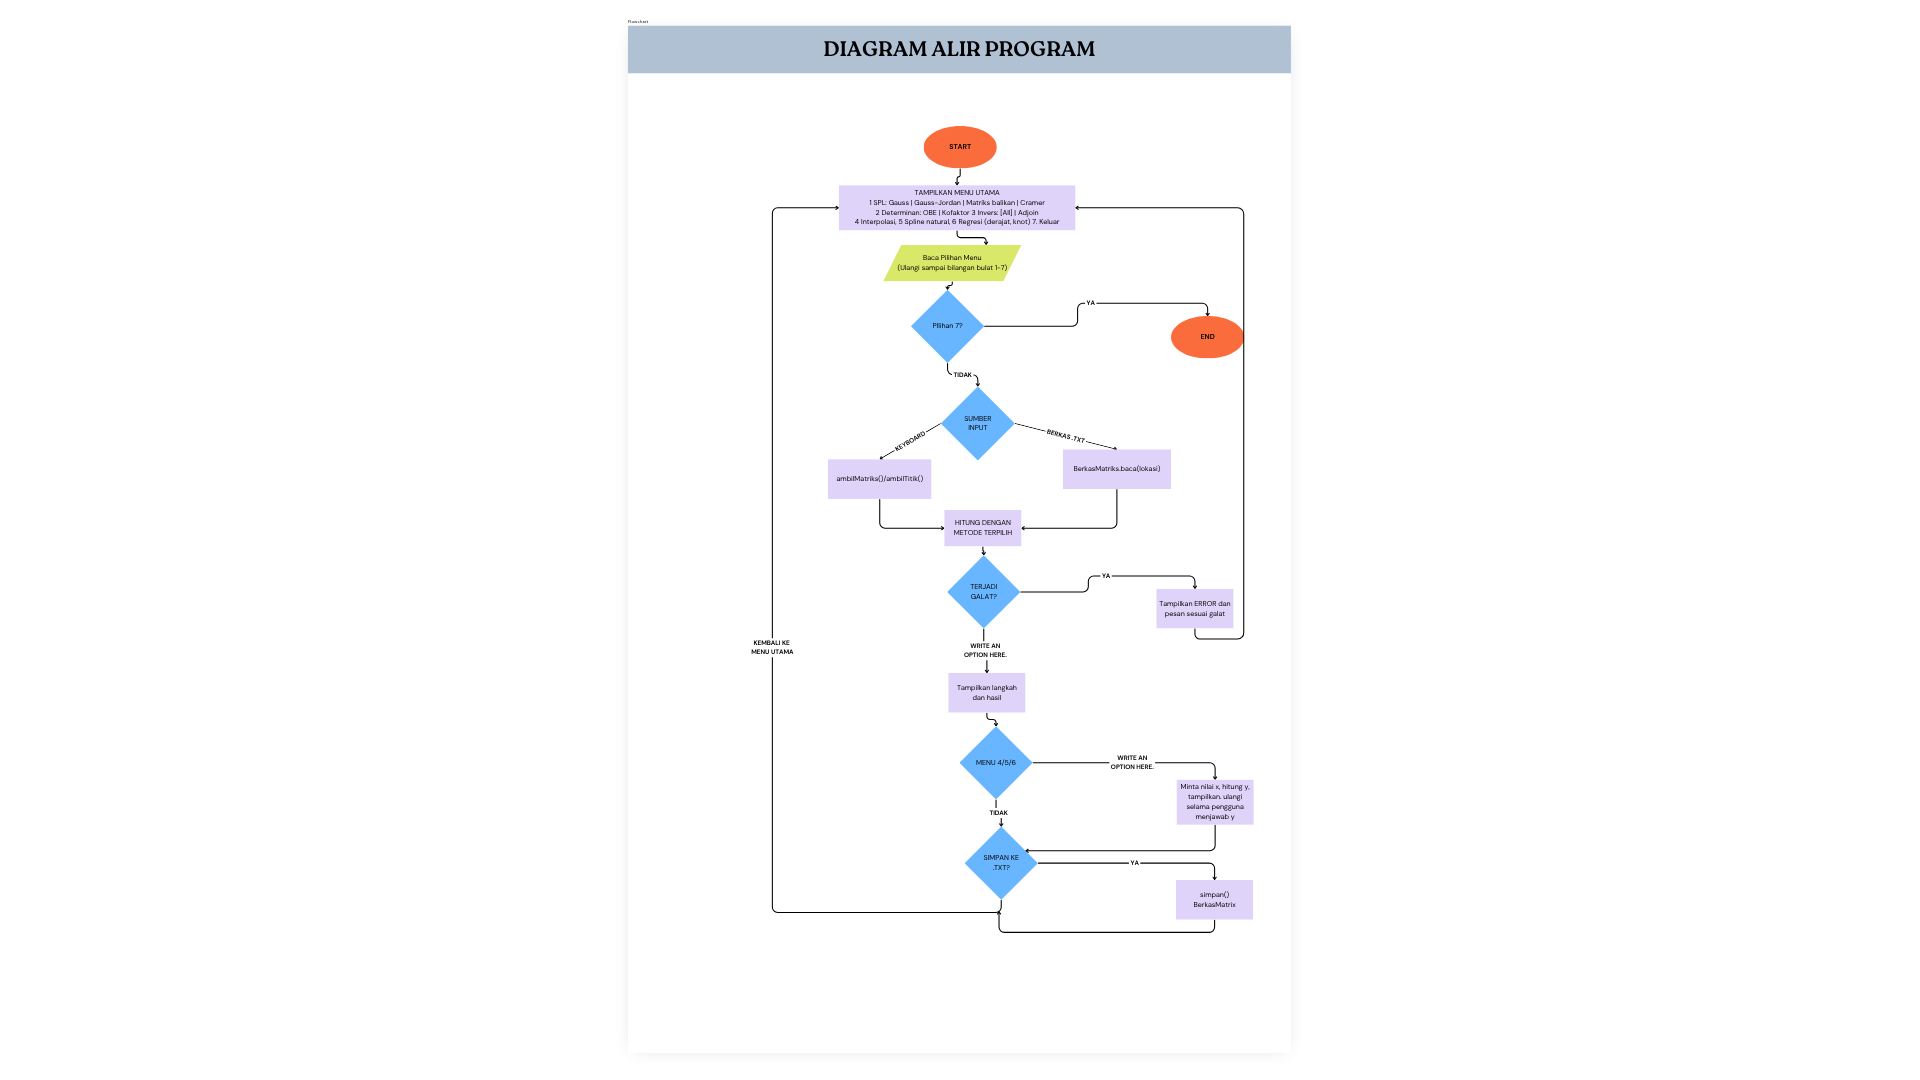
\includegraphics[width=0.8\linewidth]{imgs/Diagram alur.png}
    \caption{Diagram alir program utama}
    \label{fig:alur}
\end{figure}
\FloatBarrier

\subsection{Penggunaan Maven dan Pembuatan Berkas JAR}
Proyek ini menggunakan Apache Maven sebagai kakas manajemen (\textit{build tool}). Struktur direktori proyek mengikuti standar Maven, dengan kode sumber berada pada struktur \texttt{src/main/java/}. Seluruh konfigurasi proyek dan dependensi diatur secara terpusat di dalam berkas \texttt{pom.xml}.

Untuk melakukan kompilasi dan mengemas program menjadi berkas biner (\textit{ex\-e\-cut\-a\-ble}), digunakan perintah berikut pada terminal:
\begin{keluaran}
mvn clean package
\end{keluaran}

Perintah tersebut akan membersihkan \textit{build} sebelumnya, mengompilasi ulang seluruh kode sumber, dan membungkusnya menjadi berkas \texttt{.jar} (misalnya \texttt{Algeo-}\allowbreak\texttt{1.0.jar}). Berkas hasil kompilasi tersebut akan diletakkan secara otomatis di dalam direktori \texttt{target/}. Berkas biner ini bersifat portabel dan dapat dijalankan langsung menggunakan perintah:
\begin{keluaran}
java -jar target/<nama-file>.jar
\end{keluaran}


% BAB 4 -- EKSPERIMEN
\section{Eksperimen}
Berikut hasil eksekusi program terhadap seluruh kasus uji pada spesifikasi.

\subsection{Determinan Matriks}
Diuji dengan kedua metode: reduksi baris (OBE) dan ekspansi kofaktor.
\subsubsection{Kasus Uji 1}
\begin{equation}
    \begin{bmatrix}
        0 & 2 & -1 & 3 \\
        4 & 1 & 2 & -2 \\
        -2 & 3 & 0 & 1 \\
        1 & -1 & 5 & 2 \\
    \end{bmatrix}
\end{equation}
\begin{keluaran}
1. Metode Reduksi Baris/OBE
Output:
Terminal:
Nilai determinan = -259,000

File .txt:
Metode perhitungan determinan: Reduksi Baris / OBE

Menghitung Determinan Matriks Dengan Metode Reduksi Baris/OBE
Matriks Awal:
0,000 2,000 -1,000 3,000 
4,000 1,000 2,000 -2,000 
-2,000 3,000 0,000 1,000 
1,000 -1,000 5,000 2,000 

Baris 1 ditukar dengan baris 2
4,000 1,000 2,000 -2,000 
0,000 2,000 -1,000 3,000 
-2,000 3,000 0,000 1,000 
1,000 -1,000 5,000 2,000 
Jumlah pertukaran baris = 1
B3 = B3 - (-0,500) x B1
B4 = B4 - (0,250) x B1

Matriks setelah di lakukan obe: 
4,000 1,000 2,000 -2,000 
0,000 2,000 -1,000 3,000 
0,000 3,500 1,000 0,000 
0,000 -1,250 4,500 2,500 

Baris 2 ditukar dengan baris 3
4,000 1,000 2,000 -2,000 
0,000 3,500 1,000 0,000 
0,000 2,000 -1,000 3,000 
0,000 -1,250 4,500 2,500 
Jumlah pertukaran baris = 2
B3 = B3 - (0,571) x B2
B4 = B4 - (-0,357) x B2

Matriks setelah di lakukan obe: 
4,000 1,000 2,000 -2,000 
0,000 3,500 1,000 0,000 
0,000 0,000 -1,571 3,000 
0,000 0,000 4,857 2,500 

Baris 3 ditukar dengan baris 4
4,000 1,000 2,000 -2,000 
0,000 3,500 1,000 0,000 
0,000 0,000 4,857 2,500 
0,000 0,000 -1,571 3,000 
Jumlah pertukaran baris = 3
B4 = B4 - (-0,324) x B3

Matriks setelah di lakukan obe: 
4,000 1,000 2,000 -2,000 
0,000 3,500 1,000 0,000 
0,000 0,000 4,857 2,500 
0,000 0,000 0,000 3,809 

Matriks setelah di lakukan obe: 
4,000 1,000 2,000 -2,000 
0,000 3,500 1,000 0,000 
0,000 0,000 4,857 2,500 
0,000 0,000 0,000 3,809 
Determinan = -259,000

Input matriks:
0,000	2,000	-1,000	3,000
4,000	1,000	2,000	-2,000
-2,000	3,000	0,000	1,000
1,000	-1,000	5,000	2,000

Nilai determinan = -259,000

2. Metode Ekspansi Kofaktor
Output:
Terminal:
Nilai determinan = -259,000

File .txt:
Metode perhitungan determinan: Ekspansi Kofaktor

Menghitung Determinan Matriks Dengan Ekspansi Kofaktor

Perhitungan Matriks (4x4)
0,000 2,000 -1,000 3,000 
4,000 1,000 2,000 -2,000 
-2,000 3,000 0,000 1,000 
1,000 -1,000 5,000 2,000 
>> Ekspansi kofaktor pada baris: 1

Elemen m[1][1] = 0,000
Elemen bernilai 0 (Dilewati)


Elemen m[1][2] = 2,000
Submatriks kofaktor setelah menghapus Baris 1 & Kolom 2:
4,000 2,000 -2,000 
-2,000 0,000 1,000 
1,000 5,000 2,000 

Perhitungan Matriks (3x3)
4,000 2,000 -2,000 
-2,000 0,000 1,000 
1,000 5,000 2,000 
>> Ekspansi kofaktor pada baris: 2

Elemen m[2][1] = (-2,000)
Submatriks kofaktor setelah menghapus Baris 2 & Kolom 1:
2,000 -2,000 
5,000 2,000 

Perhitungan Matriks (2x2)
2,000 -2,000 
5,000 2,000 
Matriks 2x2, Determinan = (2,000 * 2,000) - ((-2,000) * 5,000) = 14,000
Kofaktor C[2][1] = (-1) * 14,000 = (-14,000)
Hasil Perkalian m[2][1] * C[2][1] = (-2,000) * (-14,000) = 28,000

Elemen m[2][2] = 0,000
Elemen bernilai 0 (Dilewati)


Elemen m[2][3] = 1,000
Submatriks kofaktor setelah menghapus Baris 2 & Kolom 3:
4,000 2,000 
1,000 5,000 

Perhitungan Matriks (2x2)
4,000 2,000 
1,000 5,000 
Matriks 2x2, Determinan = (4,000 * 5,000) - (2,000 * 1,000) = 18,000
Kofaktor C[2][3] = (-1) * 18,000 = (-18,000)
Hasil Perkalian m[2][3] * C[2][3] = 1,000 * (-18,000) = (-18,000)
Hasil: 28,000 - 18,000 = 10,000
Total Determinan Sub-bagian ini = 10,000

Kofaktor C[1][2] = (-1) * 10,000 = (-10,000)
Hasil Perkalian m[1][2] * C[1][2] = 2,000 * (-10,000) = (-20,000)

Elemen m[1][3] = (-1,000)
Submatriks kofaktor setelah menghapus Baris 1 & Kolom 3:
4,000 1,000 -2,000 
-2,000 3,000 1,000 
1,000 -1,000 2,000 

Perhitungan Matriks (3x3)
4,000 1,000 -2,000 
-2,000 3,000 1,000 
1,000 -1,000 2,000 
>> Ekspansi kofaktor pada baris: 1

Elemen m[1][1] = 4,000
Submatriks kofaktor setelah menghapus Baris 1 & Kolom 1:
3,000 1,000 
-1,000 2,000 

Perhitungan Matriks (2x2)
3,000 1,000 
-1,000 2,000 
Matriks 2x2, Determinan = (3,000 * 2,000) - (1,000 * (-1,000)) = 7,000
Kofaktor C[1][1] = (+1) * 7,000 = 7,000
Hasil Perkalian m[1][1] * C[1][1] = 4,000 * 7,000 = 28,000

Elemen m[1][2] = 1,000
Submatriks kofaktor setelah menghapus Baris 1 & Kolom 2:
-2,000 1,000 
1,000 2,000 

Perhitungan Matriks (2x2)
-2,000 1,000 
1,000 2,000 
Matriks 2x2, Determinan = ((-2,000) * 2,000) - (1,000 * 1,000) = (-5,000)
Kofaktor C[1][2] = (-1) * (-5,000) = 5,000
Hasil Perkalian m[1][2] * C[1][2] = 1,000 * 5,000 = 5,000

Elemen m[1][3] = (-2,000)
Submatriks kofaktor setelah menghapus Baris 1 & Kolom 3:
-2,000 3,000 
1,000 -1,000 

Perhitungan Matriks (2x2)
-2,000 3,000 
1,000 -1,000 
Matriks 2x2, Determinan = ((-2,000) * (-1,000)) - (3,000 * 1,000) = (-1,000)
Kofaktor C[1][3] = (+1) * (-1,000) = (-1,000)
Hasil Perkalian m[1][3] * C[1][3] = (-2,000) * (-1,000) = 2,000
Hasil: 28,000 + 5,000 + 2,000 = 35,000
Total Determinan Sub-bagian ini = 35,000

Kofaktor C[1][3] = (+1) * 35,000 = 35,000
Hasil Perkalian m[1][3] * C[1][3] = (-1,000) * 35,000 = (-35,000)

Elemen m[1][4] = 3,000
Submatriks kofaktor setelah menghapus Baris 1 & Kolom 4:
4,000 1,000 2,000 
-2,000 3,000 0,000 
1,000 -1,000 5,000 

Perhitungan Matriks (3x3)
4,000 1,000 2,000 
-2,000 3,000 0,000 
1,000 -1,000 5,000 
>> Ekspansi kofaktor pada baris: 2

Elemen m[2][1] = (-2,000)
Submatriks kofaktor setelah menghapus Baris 2 & Kolom 1:
1,000 2,000 
-1,000 5,000 

Perhitungan Matriks (2x2)
1,000 2,000 
-1,000 5,000 
Matriks 2x2, Determinan = (1,000 * 5,000) - (2,000 * (-1,000)) = 7,000
Kofaktor C[2][1] = (-1) * 7,000 = (-7,000)
Hasil Perkalian m[2][1] * C[2][1] = (-2,000) * (-7,000) = 14,000

Elemen m[2][2] = 3,000
Submatriks kofaktor setelah menghapus Baris 2 & Kolom 2:
4,000 2,000 
1,000 5,000 

Perhitungan Matriks (2x2)
4,000 2,000 
1,000 5,000 
Matriks 2x2, Determinan = (4,000 * 5,000) - (2,000 * 1,000) = 18,000
Kofaktor C[2][2] = (+1) * 18,000 = 18,000
Hasil Perkalian m[2][2] * C[2][2] = 3,000 * 18,000 = 54,000

Elemen m[2][3] = 0,000
Elemen bernilai 0 (Dilewati)

Hasil: 14,000 + 54,000 = 68,000
Total Determinan Sub-bagian ini = 68,000

Kofaktor C[1][4] = (-1) * 68,000 = (-68,000)
Hasil Perkalian m[1][4] * C[1][4] = 3,000 * (-68,000) = (-204,000)
Hasil: (-20,000) - 35,000 - 204,000 = (-259,000)
Total Determinan Sub-bagian ini = (-259,000)


Input matriks:
0,000	2,000	-1,000	3,000
4,000	1,000	2,000	-2,000
-2,000	3,000	0,000	1,000
1,000	-1,000	5,000	2,000

Nilai determinan = -259,000
\end{keluaran}
Analisis untuk kasus uji 1, hasil yang dihasilkan antara kedua metode sama.
\subsubsection{Kasus Uji 2}
\begin{equation}
    \begin{bmatrix}
        2 & -1 & 3 & 0 & 4 \\
        1 & 2 & -2 & 5 & -1 \\
        3 & 1 & 1 & 2 & 0 \\
        0 & 4 & -1 & 3 & 2 \\
        5 & 0 & 4 & 2 & 4 \\
    \end{bmatrix}
\end{equation}
\begin{keluaran}
1. Metode Reduksi Baris/OBE
Output:
Terminal:
Nilai determinan = 0,000

File .txt:
Metode perhitungan determinan: Reduksi Baris / OBE

Menghitung Determinan Matriks Dengan Metode Reduksi Baris/OBE
Matriks Awal:
2,000 -1,000 3,000 0,000 4,000 
1,000 2,000 -2,000 5,000 -1,000 
3,000 1,000 1,000 2,000 0,000 
0,000 4,000 -1,000 3,000 2,000 
5,000 0,000 4,000 2,000 4,000 

Baris 1 ditukar dengan baris 5
5,000 0,000 4,000 2,000 4,000 
1,000 2,000 -2,000 5,000 -1,000 
3,000 1,000 1,000 2,000 0,000 
0,000 4,000 -1,000 3,000 2,000 
2,000 -1,000 3,000 0,000 4,000 
Jumlah pertukaran baris = 1
B2 = B2 - (0,200) x B1
B3 = B3 - (0,600) x B1
B5 = B5 - (0,400) x B1

Matriks setelah di lakukan obe: 
5,000 0,000 4,000 2,000 4,000 
0,000 2,000 -2,800 4,600 -1,800 
0,000 1,000 -1,400 0,800 -2,400 
0,000 4,000 -1,000 3,000 2,000 
0,000 -1,000 1,400 -0,800 2,400 

Baris 2 ditukar dengan baris 4
5,000 0,000 4,000 2,000 4,000 
0,000 4,000 -1,000 3,000 2,000 
0,000 1,000 -1,400 0,800 -2,400 
0,000 2,000 -2,800 4,600 -1,800 
0,000 -1,000 1,400 -0,800 2,400 
Jumlah pertukaran baris = 2
B3 = B3 - (0,250) x B2
B4 = B4 - (0,500) x B2
B5 = B5 - (-0,250) x B2

Matriks setelah di lakukan obe: 
5,000 0,000 4,000 2,000 4,000 
0,000 4,000 -1,000 3,000 2,000 
0,000 0,000 -1,150 0,050 -2,900 
0,000 0,000 -2,300 3,100 -2,800 
0,000 0,000 1,150 -0,050 2,900 

Baris 3 ditukar dengan baris 4
5,000 0,000 4,000 2,000 4,000 
0,000 4,000 -1,000 3,000 2,000 
0,000 0,000 -2,300 3,100 -2,800 
0,000 0,000 -1,150 0,050 -2,900 
0,000 0,000 1,150 -0,050 2,900 
Jumlah pertukaran baris = 3
B4 = B4 - (0,500) x B3
B5 = B5 - (-0,500) x B3

Matriks setelah di lakukan obe: 
5,000 0,000 4,000 2,000 4,000 
0,000 4,000 -1,000 3,000 2,000 
0,000 0,000 -2,300 3,100 -2,800 
0,000 0,000 0,000 -1,500 -1,500 
0,000 0,000 0,000 1,500 1,500 
B5 = B5 - (-1,000) x B4

Matriks setelah di lakukan obe: 
5,000 0,000 4,000 2,000 4,000 
0,000 4,000 -1,000 3,000 2,000 
0,000 0,000 -2,300 3,100 -2,800 
0,000 0,000 0,000 -1,500 -1,500 
0,000 0,000 0,000 0,000 0,000 
Kolom/Baris 5 semuanya bernilai 0, determinan = 0

Input matriks:
2,000	-1,000	3,000	0,000	4,000
1,000	2,000	-2,000	5,000	-1,000
3,000	1,000	1,000	2,000	0,000
0,000	4,000	-1,000	3,000	2,000
5,000	0,000	4,000	2,000	4,000

Nilai determinan = 0,000

2. Metode Ekspansi Kofaktor
Output:
Terminal:
Nilai determinan = 0,000

File .txt:
Metode perhitungan determinan: Ekspansi Kofaktor

Menghitung Determinan Matriks Dengan Ekspansi Kofaktor

Perhitungan Matriks (5x5)
2,000 -1,000 3,000 0,000 4,000 
1,000 2,000 -2,000 5,000 -1,000 
3,000 1,000 1,000 2,000 0,000 
0,000 4,000 -1,000 3,000 2,000 
5,000 0,000 4,000 2,000 4,000 
>> Ekspansi kofaktor pada baris: 1

Elemen m[1][1] = 2,000
Submatriks kofaktor setelah menghapus Baris 1 & Kolom 1:
2,000 -2,000 5,000 -1,000 
1,000 1,000 2,000 0,000 
4,000 -1,000 3,000 2,000 
0,000 4,000 2,000 4,000 

Perhitungan Matriks (4x4)
2,000 -2,000 5,000 -1,000 
1,000 1,000 2,000 0,000 
4,000 -1,000 3,000 2,000 
0,000 4,000 2,000 4,000 
>> Ekspansi kofaktor pada baris: 2

Elemen m[2][1] = 1,000
Submatriks kofaktor setelah menghapus Baris 2 & Kolom 1:
-2,000 5,000 -1,000 
-1,000 3,000 2,000 
4,000 2,000 4,000 

Perhitungan Matriks (3x3)
-2,000 5,000 -1,000 
-1,000 3,000 2,000 
4,000 2,000 4,000 
>> Ekspansi kofaktor pada baris: 1

Elemen m[1][1] = (-2,000)
Submatriks kofaktor setelah menghapus Baris 1 & Kolom 1:
3,000 2,000 
2,000 4,000 

Perhitungan Matriks (2x2)
3,000 2,000 
2,000 4,000 
Matriks 2x2, Determinan = (3,000 * 4,000) - (2,000 * 2,000) = 8,000
Kofaktor C[1][1] = (+1) * 8,000 = 8,000
Hasil Perkalian m[1][1] * C[1][1] = (-2,000) * 8,000 = (-16,000)

Elemen m[1][2] = 5,000
Submatriks kofaktor setelah menghapus Baris 1 & Kolom 2:
-1,000 2,000 
4,000 4,000 

Perhitungan Matriks (2x2)
-1,000 2,000 
4,000 4,000 
Matriks 2x2, Determinan = ((-1,000) * 4,000) - (2,000 * 4,000) = (-12,000)
Kofaktor C[1][2] = (-1) * (-12,000) = 12,000
Hasil Perkalian m[1][2] * C[1][2] = 5,000 * 12,000 = 60,000

Elemen m[1][3] = (-1,000)
Submatriks kofaktor setelah menghapus Baris 1 & Kolom 3:
-1,000 3,000 
4,000 2,000 

Perhitungan Matriks (2x2)
-1,000 3,000 
4,000 2,000 
Matriks 2x2, Determinan = ((-1,000) * 2,000) - (3,000 * 4,000) = (-14,000)
Kofaktor C[1][3] = (+1) * (-14,000) = (-14,000)
Hasil Perkalian m[1][3] * C[1][3] = (-1,000) * (-14,000) = 14,000
Hasil: (-16,000) + 60,000 + 14,000 = 58,000
Total Determinan Sub-bagian ini = 58,000

Kofaktor C[2][1] = (-1) * 58,000 = (-58,000)
Hasil Perkalian m[2][1] * C[2][1] = 1,000 * (-58,000) = (-58,000)

Elemen m[2][2] = 1,000
Submatriks kofaktor setelah menghapus Baris 2 & Kolom 2:
2,000 5,000 -1,000 
4,000 3,000 2,000 
0,000 2,000 4,000 

Perhitungan Matriks (3x3)
2,000 5,000 -1,000 
4,000 3,000 2,000 
0,000 2,000 4,000 
>> Ekspansi kofaktor pada baris: 3

Elemen m[3][1] = 0,000
Elemen bernilai 0 (Dilewati)


Elemen m[3][2] = 2,000
Submatriks kofaktor setelah menghapus Baris 3 & Kolom 2:
2,000 -1,000 
4,000 2,000 

Perhitungan Matriks (2x2)
2,000 -1,000 
4,000 2,000 
Matriks 2x2, Determinan = (2,000 * 2,000) - ((-1,000) * 4,000) = 8,000
Kofaktor C[3][2] = (-1) * 8,000 = (-8,000)
Hasil Perkalian m[3][2] * C[3][2] = 2,000 * (-8,000) = (-16,000)

Elemen m[3][3] = 4,000
Submatriks kofaktor setelah menghapus Baris 3 & Kolom 3:
2,000 5,000 
4,000 3,000 

Perhitungan Matriks (2x2)
2,000 5,000 
4,000 3,000 
Matriks 2x2, Determinan = (2,000 * 3,000) - (5,000 * 4,000) = (-14,000)
Kofaktor C[3][3] = (+1) * (-14,000) = (-14,000)
Hasil Perkalian m[3][3] * C[3][3] = 4,000 * (-14,000) = (-56,000)
Hasil: (-16,000) - 56,000 = (-72,000)
Total Determinan Sub-bagian ini = (-72,000)

Kofaktor C[2][2] = (+1) * (-72,000) = (-72,000)
Hasil Perkalian m[2][2] * C[2][2] = 1,000 * (-72,000) = (-72,000)

Elemen m[2][3] = 2,000
Submatriks kofaktor setelah menghapus Baris 2 & Kolom 3:
2,000 -2,000 -1,000 
4,000 -1,000 2,000 
0,000 4,000 4,000 

Perhitungan Matriks (3x3)
2,000 -2,000 -1,000 
4,000 -1,000 2,000 
0,000 4,000 4,000 
>> Ekspansi kofaktor pada baris: 3

Elemen m[3][1] = 0,000
Elemen bernilai 0 (Dilewati)


Elemen m[3][2] = 4,000
Submatriks kofaktor setelah menghapus Baris 3 & Kolom 2:
2,000 -1,000 
4,000 2,000 

Perhitungan Matriks (2x2)
2,000 -1,000 
4,000 2,000 
Matriks 2x2, Determinan = (2,000 * 2,000) - ((-1,000) * 4,000) = 8,000
Kofaktor C[3][2] = (-1) * 8,000 = (-8,000)
Hasil Perkalian m[3][2] * C[3][2] = 4,000 * (-8,000) = (-32,000)

Elemen m[3][3] = 4,000
Submatriks kofaktor setelah menghapus Baris 3 & Kolom 3:
2,000 -2,000 
4,000 -1,000 

Perhitungan Matriks (2x2)
2,000 -2,000 
4,000 -1,000 
Matriks 2x2, Determinan = (2,000 * (-1,000)) - ((-2,000) * 4,000) = 6,000
Kofaktor C[3][3] = (+1) * 6,000 = 6,000
Hasil Perkalian m[3][3] * C[3][3] = 4,000 * 6,000 = 24,000
Hasil: (-32,000) + 24,000 = (-8,000)
Total Determinan Sub-bagian ini = (-8,000)

Kofaktor C[2][3] = (-1) * (-8,000) = 8,000
Hasil Perkalian m[2][3] * C[2][3] = 2,000 * 8,000 = 16,000

Elemen m[2][4] = 0,000
Elemen bernilai 0 (Dilewati)

Hasil: (-58,000) - 72,000 + 16,000 = (-114,000)
Total Determinan Sub-bagian ini = (-114,000)

Kofaktor C[1][1] = (+1) * (-114,000) = (-114,000)
Hasil Perkalian m[1][1] * C[1][1] = 2,000 * (-114,000) = (-228,000)

Elemen m[1][2] = (-1,000)
Submatriks kofaktor setelah menghapus Baris 1 & Kolom 2:
1,000 -2,000 5,000 -1,000 
3,000 1,000 2,000 0,000 
0,000 -1,000 3,000 2,000 
5,000 4,000 2,000 4,000 

Perhitungan Matriks (4x4)
1,000 -2,000 5,000 -1,000 
3,000 1,000 2,000 0,000 
0,000 -1,000 3,000 2,000 
5,000 4,000 2,000 4,000 
>> Ekspansi kofaktor pada baris: 2

Elemen m[2][1] = 3,000
Submatriks kofaktor setelah menghapus Baris 2 & Kolom 1:
-2,000 5,000 -1,000 
-1,000 3,000 2,000 
4,000 2,000 4,000 

Perhitungan Matriks (3x3)
-2,000 5,000 -1,000 
-1,000 3,000 2,000 
4,000 2,000 4,000 
>> Ekspansi kofaktor pada baris: 1

Elemen m[1][1] = (-2,000)
Submatriks kofaktor setelah menghapus Baris 1 & Kolom 1:
3,000 2,000 
2,000 4,000 

Perhitungan Matriks (2x2)
3,000 2,000 
2,000 4,000 
Matriks 2x2, Determinan = (3,000 * 4,000) - (2,000 * 2,000) = 8,000
Kofaktor C[1][1] = (+1) * 8,000 = 8,000
Hasil Perkalian m[1][1] * C[1][1] = (-2,000) * 8,000 = (-16,000)

Elemen m[1][2] = 5,000
Submatriks kofaktor setelah menghapus Baris 1 & Kolom 2:
-1,000 2,000 
4,000 4,000 

Perhitungan Matriks (2x2)
-1,000 2,000 
4,000 4,000 
Matriks 2x2, Determinan = ((-1,000) * 4,000) - (2,000 * 4,000) = (-12,000)
Kofaktor C[1][2] = (-1) * (-12,000) = 12,000
Hasil Perkalian m[1][2] * C[1][2] = 5,000 * 12,000 = 60,000

Elemen m[1][3] = (-1,000)
Submatriks kofaktor setelah menghapus Baris 1 & Kolom 3:
-1,000 3,000 
4,000 2,000 

Perhitungan Matriks (2x2)
-1,000 3,000 
4,000 2,000 
Matriks 2x2, Determinan = ((-1,000) * 2,000) - (3,000 * 4,000) = (-14,000)
Kofaktor C[1][3] = (+1) * (-14,000) = (-14,000)
Hasil Perkalian m[1][3] * C[1][3] = (-1,000) * (-14,000) = 14,000
Hasil: (-16,000) + 60,000 + 14,000 = 58,000
Total Determinan Sub-bagian ini = 58,000

Kofaktor C[2][1] = (-1) * 58,000 = (-58,000)
Hasil Perkalian m[2][1] * C[2][1] = 3,000 * (-58,000) = (-174,000)

Elemen m[2][2] = 1,000
Submatriks kofaktor setelah menghapus Baris 2 & Kolom 2:
1,000 5,000 -1,000 
0,000 3,000 2,000 
5,000 2,000 4,000 

Perhitungan Matriks (3x3)
1,000 5,000 -1,000 
0,000 3,000 2,000 
5,000 2,000 4,000 
>> Ekspansi kofaktor pada baris: 2

Elemen m[2][1] = 0,000
Elemen bernilai 0 (Dilewati)


Elemen m[2][2] = 3,000
Submatriks kofaktor setelah menghapus Baris 2 & Kolom 2:
1,000 -1,000 
5,000 4,000 

Perhitungan Matriks (2x2)
1,000 -1,000 
5,000 4,000 
Matriks 2x2, Determinan = (1,000 * 4,000) - ((-1,000) * 5,000) = 9,000
Kofaktor C[2][2] = (+1) * 9,000 = 9,000
Hasil Perkalian m[2][2] * C[2][2] = 3,000 * 9,000 = 27,000

Elemen m[2][3] = 2,000
Submatriks kofaktor setelah menghapus Baris 2 & Kolom 3:
1,000 5,000 
5,000 2,000 

Perhitungan Matriks (2x2)
1,000 5,000 
5,000 2,000 
Matriks 2x2, Determinan = (1,000 * 2,000) - (5,000 * 5,000) = (-23,000)
Kofaktor C[2][3] = (-1) * (-23,000) = 23,000
Hasil Perkalian m[2][3] * C[2][3] = 2,000 * 23,000 = 46,000
Hasil: 27,000 + 46,000 = 73,000
Total Determinan Sub-bagian ini = 73,000

Kofaktor C[2][2] = (+1) * 73,000 = 73,000
Hasil Perkalian m[2][2] * C[2][2] = 1,000 * 73,000 = 73,000

Elemen m[2][3] = 2,000
Submatriks kofaktor setelah menghapus Baris 2 & Kolom 3:
1,000 -2,000 -1,000 
0,000 -1,000 2,000 
5,000 4,000 4,000 

Perhitungan Matriks (3x3)
1,000 -2,000 -1,000 
0,000 -1,000 2,000 
5,000 4,000 4,000 
>> Ekspansi kofaktor pada baris: 2

Elemen m[2][1] = 0,000
Elemen bernilai 0 (Dilewati)


Elemen m[2][2] = (-1,000)
Submatriks kofaktor setelah menghapus Baris 2 & Kolom 2:
1,000 -1,000 
5,000 4,000 

Perhitungan Matriks (2x2)
1,000 -1,000 
5,000 4,000 
Matriks 2x2, Determinan = (1,000 * 4,000) - ((-1,000) * 5,000) = 9,000
Kofaktor C[2][2] = (+1) * 9,000 = 9,000
Hasil Perkalian m[2][2] * C[2][2] = (-1,000) * 9,000 = (-9,000)

Elemen m[2][3] = 2,000
Submatriks kofaktor setelah menghapus Baris 2 & Kolom 3:
1,000 -2,000 
5,000 4,000 

Perhitungan Matriks (2x2)
1,000 -2,000 
5,000 4,000 
Matriks 2x2, Determinan = (1,000 * 4,000) - ((-2,000) * 5,000) = 14,000
Kofaktor C[2][3] = (-1) * 14,000 = (-14,000)
Hasil Perkalian m[2][3] * C[2][3] = 2,000 * (-14,000) = (-28,000)
Hasil: (-9,000) - 28,000 = (-37,000)
Total Determinan Sub-bagian ini = (-37,000)

Kofaktor C[2][3] = (-1) * (-37,000) = 37,000
Hasil Perkalian m[2][3] * C[2][3] = 2,000 * 37,000 = 74,000

Elemen m[2][4] = 0,000
Elemen bernilai 0 (Dilewati)

Hasil: (-174,000) + 73,000 + 74,000 = (-27,000)
Total Determinan Sub-bagian ini = (-27,000)

Kofaktor C[1][2] = (-1) * (-27,000) = 27,000
Hasil Perkalian m[1][2] * C[1][2] = (-1,000) * 27,000 = (-27,000)

Elemen m[1][3] = 3,000
Submatriks kofaktor setelah menghapus Baris 1 & Kolom 3:
1,000 2,000 5,000 -1,000 
3,000 1,000 2,000 0,000 
0,000 4,000 3,000 2,000 
5,000 0,000 2,000 4,000 

Perhitungan Matriks (4x4)
1,000 2,000 5,000 -1,000 
3,000 1,000 2,000 0,000 
0,000 4,000 3,000 2,000 
5,000 0,000 2,000 4,000 
>> Ekspansi kofaktor pada baris: 2

Elemen m[2][1] = 3,000
Submatriks kofaktor setelah menghapus Baris 2 & Kolom 1:
2,000 5,000 -1,000 
4,000 3,000 2,000 
0,000 2,000 4,000 

Perhitungan Matriks (3x3)
2,000 5,000 -1,000 
4,000 3,000 2,000 
0,000 2,000 4,000 
>> Ekspansi kofaktor pada baris: 3

Elemen m[3][1] = 0,000
Elemen bernilai 0 (Dilewati)


Elemen m[3][2] = 2,000
Submatriks kofaktor setelah menghapus Baris 3 & Kolom 2:
2,000 -1,000 
4,000 2,000 

Perhitungan Matriks (2x2)
2,000 -1,000 
4,000 2,000 
Matriks 2x2, Determinan = (2,000 * 2,000) - ((-1,000) * 4,000) = 8,000
Kofaktor C[3][2] = (-1) * 8,000 = (-8,000)
Hasil Perkalian m[3][2] * C[3][2] = 2,000 * (-8,000) = (-16,000)

Elemen m[3][3] = 4,000
Submatriks kofaktor setelah menghapus Baris 3 & Kolom 3:
2,000 5,000 
4,000 3,000 

Perhitungan Matriks (2x2)
2,000 5,000 
4,000 3,000 
Matriks 2x2, Determinan = (2,000 * 3,000) - (5,000 * 4,000) = (-14,000)
Kofaktor C[3][3] = (+1) * (-14,000) = (-14,000)
Hasil Perkalian m[3][3] * C[3][3] = 4,000 * (-14,000) = (-56,000)
Hasil: (-16,000) - 56,000 = (-72,000)
Total Determinan Sub-bagian ini = (-72,000)

Kofaktor C[2][1] = (-1) * (-72,000) = 72,000
Hasil Perkalian m[2][1] * C[2][1] = 3,000 * 72,000 = 216,000

Elemen m[2][2] = 1,000
Submatriks kofaktor setelah menghapus Baris 2 & Kolom 2:
1,000 5,000 -1,000 
0,000 3,000 2,000 
5,000 2,000 4,000 

Perhitungan Matriks (3x3)
1,000 5,000 -1,000 
0,000 3,000 2,000 
5,000 2,000 4,000 
>> Ekspansi kofaktor pada baris: 2

Elemen m[2][1] = 0,000
Elemen bernilai 0 (Dilewati)


Elemen m[2][2] = 3,000
Submatriks kofaktor setelah menghapus Baris 2 & Kolom 2:
1,000 -1,000 
5,000 4,000 

Perhitungan Matriks (2x2)
1,000 -1,000 
5,000 4,000 
Matriks 2x2, Determinan = (1,000 * 4,000) - ((-1,000) * 5,000) = 9,000
Kofaktor C[2][2] = (+1) * 9,000 = 9,000
Hasil Perkalian m[2][2] * C[2][2] = 3,000 * 9,000 = 27,000

Elemen m[2][3] = 2,000
Submatriks kofaktor setelah menghapus Baris 2 & Kolom 3:
1,000 5,000 
5,000 2,000 

Perhitungan Matriks (2x2)
1,000 5,000 
5,000 2,000 
Matriks 2x2, Determinan = (1,000 * 2,000) - (5,000 * 5,000) = (-23,000)
Kofaktor C[2][3] = (-1) * (-23,000) = 23,000
Hasil Perkalian m[2][3] * C[2][3] = 2,000 * 23,000 = 46,000
Hasil: 27,000 + 46,000 = 73,000
Total Determinan Sub-bagian ini = 73,000

Kofaktor C[2][2] = (+1) * 73,000 = 73,000
Hasil Perkalian m[2][2] * C[2][2] = 1,000 * 73,000 = 73,000

Elemen m[2][3] = 2,000
Submatriks kofaktor setelah menghapus Baris 2 & Kolom 3:
1,000 2,000 -1,000 
0,000 4,000 2,000 
5,000 0,000 4,000 

Perhitungan Matriks (3x3)
1,000 2,000 -1,000 
0,000 4,000 2,000 
5,000 0,000 4,000 
>> Ekspansi kofaktor pada baris: 2

Elemen m[2][1] = 0,000
Elemen bernilai 0 (Dilewati)


Elemen m[2][2] = 4,000
Submatriks kofaktor setelah menghapus Baris 2 & Kolom 2:
1,000 -1,000 
5,000 4,000 

Perhitungan Matriks (2x2)
1,000 -1,000 
5,000 4,000 
Matriks 2x2, Determinan = (1,000 * 4,000) - ((-1,000) * 5,000) = 9,000
Kofaktor C[2][2] = (+1) * 9,000 = 9,000
Hasil Perkalian m[2][2] * C[2][2] = 4,000 * 9,000 = 36,000

Elemen m[2][3] = 2,000
Submatriks kofaktor setelah menghapus Baris 2 & Kolom 3:
1,000 2,000 
5,000 0,000 

Perhitungan Matriks (2x2)
1,000 2,000 
5,000 0,000 
Matriks 2x2, Determinan = (1,000 * 0,000) - (2,000 * 5,000) = (-10,000)
Kofaktor C[2][3] = (-1) * (-10,000) = 10,000
Hasil Perkalian m[2][3] * C[2][3] = 2,000 * 10,000 = 20,000
Hasil: 36,000 + 20,000 = 56,000
Total Determinan Sub-bagian ini = 56,000

Kofaktor C[2][3] = (-1) * 56,000 = (-56,000)
Hasil Perkalian m[2][3] * C[2][3] = 2,000 * (-56,000) = (-112,000)

Elemen m[2][4] = 0,000
Elemen bernilai 0 (Dilewati)

Hasil: 216,000 + 73,000 - 112,000 = 177,000
Total Determinan Sub-bagian ini = 177,000

Kofaktor C[1][3] = (+1) * 177,000 = 177,000
Hasil Perkalian m[1][3] * C[1][3] = 3,000 * 177,000 = 531,000

Elemen m[1][4] = 0,000
Elemen bernilai 0 (Dilewati)


Elemen m[1][5] = 4,000
Submatriks kofaktor setelah menghapus Baris 1 & Kolom 5:
1,000 2,000 -2,000 5,000 
3,000 1,000 1,000 2,000 
0,000 4,000 -1,000 3,000 
5,000 0,000 4,000 2,000 

Perhitungan Matriks (4x4)
1,000 2,000 -2,000 5,000 
3,000 1,000 1,000 2,000 
0,000 4,000 -1,000 3,000 
5,000 0,000 4,000 2,000 
>> Ekspansi kofaktor pada baris: 3

Elemen m[3][1] = 0,000
Elemen bernilai 0 (Dilewati)


Elemen m[3][2] = 4,000
Submatriks kofaktor setelah menghapus Baris 3 & Kolom 2:
1,000 -2,000 5,000 
3,000 1,000 2,000 
5,000 4,000 2,000 

Perhitungan Matriks (3x3)
1,000 -2,000 5,000 
3,000 1,000 2,000 
5,000 4,000 2,000 
>> Ekspansi kofaktor pada baris: 1

Elemen m[1][1] = 1,000
Submatriks kofaktor setelah menghapus Baris 1 & Kolom 1:
1,000 2,000 
4,000 2,000 

Perhitungan Matriks (2x2)
1,000 2,000 
4,000 2,000 
Matriks 2x2, Determinan = (1,000 * 2,000) - (2,000 * 4,000) = (-6,000)
Kofaktor C[1][1] = (+1) * (-6,000) = (-6,000)
Hasil Perkalian m[1][1] * C[1][1] = 1,000 * (-6,000) = (-6,000)

Elemen m[1][2] = (-2,000)
Submatriks kofaktor setelah menghapus Baris 1 & Kolom 2:
3,000 2,000 
5,000 2,000 

Perhitungan Matriks (2x2)
3,000 2,000 
5,000 2,000 
Matriks 2x2, Determinan = (3,000 * 2,000) - (2,000 * 5,000) = (-4,000)
Kofaktor C[1][2] = (-1) * (-4,000) = 4,000
Hasil Perkalian m[1][2] * C[1][2] = (-2,000) * 4,000 = (-8,000)

Elemen m[1][3] = 5,000
Submatriks kofaktor setelah menghapus Baris 1 & Kolom 3:
3,000 1,000 
5,000 4,000 

Perhitungan Matriks (2x2)
3,000 1,000 
5,000 4,000 
Matriks 2x2, Determinan = (3,000 * 4,000) - (1,000 * 5,000) = 7,000
Kofaktor C[1][3] = (+1) * 7,000 = 7,000
Hasil Perkalian m[1][3] * C[1][3] = 5,000 * 7,000 = 35,000
Hasil: (-6,000) - 8,000 + 35,000 = 21,000
Total Determinan Sub-bagian ini = 21,000

Kofaktor C[3][2] = (-1) * 21,000 = (-21,000)
Hasil Perkalian m[3][2] * C[3][2] = 4,000 * (-21,000) = (-84,000)

Elemen m[3][3] = (-1,000)
Submatriks kofaktor setelah menghapus Baris 3 & Kolom 3:
1,000 2,000 5,000 
3,000 1,000 2,000 
5,000 0,000 2,000 

Perhitungan Matriks (3x3)
1,000 2,000 5,000 
3,000 1,000 2,000 
5,000 0,000 2,000 
>> Ekspansi kofaktor pada baris: 3

Elemen m[3][1] = 5,000
Submatriks kofaktor setelah menghapus Baris 3 & Kolom 1:
2,000 5,000 
1,000 2,000 

Perhitungan Matriks (2x2)
2,000 5,000 
1,000 2,000 
Matriks 2x2, Determinan = (2,000 * 2,000) - (5,000 * 1,000) = (-1,000)
Kofaktor C[3][1] = (+1) * (-1,000) = (-1,000)
Hasil Perkalian m[3][1] * C[3][1] = 5,000 * (-1,000) = (-5,000)

Elemen m[3][2] = 0,000
Elemen bernilai 0 (Dilewati)


Elemen m[3][3] = 2,000
Submatriks kofaktor setelah menghapus Baris 3 & Kolom 3:
1,000 2,000 
3,000 1,000 

Perhitungan Matriks (2x2)
1,000 2,000 
3,000 1,000 
Matriks 2x2, Determinan = (1,000 * 1,000) - (2,000 * 3,000) = (-5,000)
Kofaktor C[3][3] = (+1) * (-5,000) = (-5,000)
Hasil Perkalian m[3][3] * C[3][3] = 2,000 * (-5,000) = (-10,000)
Hasil: (-5,000) - 10,000 = (-15,000)
Total Determinan Sub-bagian ini = (-15,000)

Kofaktor C[3][3] = (+1) * (-15,000) = (-15,000)
Hasil Perkalian m[3][3] * C[3][3] = (-1,000) * (-15,000) = 15,000

Elemen m[3][4] = 3,000
Submatriks kofaktor setelah menghapus Baris 3 & Kolom 4:
1,000 2,000 -2,000 
3,000 1,000 1,000 
5,000 0,000 4,000 

Perhitungan Matriks (3x3)
1,000 2,000 -2,000 
3,000 1,000 1,000 
5,000 0,000 4,000 
>> Ekspansi kofaktor pada baris: 3

Elemen m[3][1] = 5,000
Submatriks kofaktor setelah menghapus Baris 3 & Kolom 1:
2,000 -2,000 
1,000 1,000 

Perhitungan Matriks (2x2)
2,000 -2,000 
1,000 1,000 
Matriks 2x2, Determinan = (2,000 * 1,000) - ((-2,000) * 1,000) = 4,000
Kofaktor C[3][1] = (+1) * 4,000 = 4,000
Hasil Perkalian m[3][1] * C[3][1] = 5,000 * 4,000 = 20,000

Elemen m[3][2] = 0,000
Elemen bernilai 0 (Dilewati)


Elemen m[3][3] = 4,000
Submatriks kofaktor setelah menghapus Baris 3 & Kolom 3:
1,000 2,000 
3,000 1,000 

Perhitungan Matriks (2x2)
1,000 2,000 
3,000 1,000 
Matriks 2x2, Determinan = (1,000 * 1,000) - (2,000 * 3,000) = (-5,000)
Kofaktor C[3][3] = (+1) * (-5,000) = (-5,000)
Hasil Perkalian m[3][3] * C[3][3] = 4,000 * (-5,000) = (-20,000)
Hasil: 20,000 - 20,000 = 0,000
Total Determinan Sub-bagian ini = 0,000

Kofaktor C[3][4] = (-1) * 0,000 = -0,000
Hasil Perkalian m[3][4] * C[3][4] = 3,000 * -0,000 = -0,000
Hasil: (-84,000) + 15,000 + -0,000 = (-69,000)
Total Determinan Sub-bagian ini = (-69,000)

Kofaktor C[1][5] = (+1) * (-69,000) = (-69,000)
Hasil Perkalian m[1][5] * C[1][5] = 4,000 * (-69,000) = (-276,000)
Hasil: (-228,000) - 27,000 + 531,000 - 276,000 = 0,000
Total Determinan Sub-bagian ini = 0,000


Input matriks:
2,000	-1,000	3,000	0,000	4,000
1,000	2,000	-2,000	5,000	-1,000
3,000	1,000	1,000	2,000	0,000
0,000	4,000	-1,000	3,000	2,000
5,000	0,000	4,000	2,000	4,000

Nilai determinan = 0,000
\end{keluaran}
Analisis untuk kasus uji 2, hasil yang dihasilkan antara kedua metode sama.
\subsubsection{Kasus Uji 3}
\begin{equation}
    \begin{bmatrix}
        0 & 2 & -1 & 3 \\
        4 & 1 & 2 & -2 \\
        -2 & 3 & 0 & 1 \\
        1 & -1 & 5 & 2 \\
    \end{bmatrix}
\end{equation}
\begin{keluaran}
1. Metode Reduksi Baris/OBE
Output: 
Terminal:
Nilai determinan = 0,010

File .txt:
Metode perhitungan determinan: Reduksi Baris / OBE

Menghitung Determinan Matriks Dengan Metode Reduksi Baris/OBE
Matriks Awal:
0,500 1,000 0,000 0,500 
0,500 1,250 0,250 0,500 
-0,100 -0,400 0,200 -0,300 
0,600 1,250 0,450 0,600 

Baris 1 ditukar dengan baris 4
0,600 1,250 0,450 0,600 
0,500 1,250 0,250 0,500 
-0,100 -0,400 0,200 -0,300 
0,500 1,000 0,000 0,500 
Jumlah pertukaran baris = 1
B2 = B2 - (0,833) x B1
B3 = B3 - (-0,167) x B1
B4 = B4 - (0,833) x B1

Matriks setelah di lakukan obe: 
0,600 1,250 0,450 0,600 
0,000 0,208 -0,125 0,000 
0,000 -0,192 0,275 -0,200 
0,000 -0,042 -0,375 0,000 
B3 = B3 - (-0,920) x B2
B4 = B4 - (-0,200) x B2

Matriks setelah di lakukan obe: 
0,600 1,250 0,450 0,600 
0,000 0,208 -0,125 0,000 
0,000 0,000 0,160 -0,200 
0,000 0,000 -0,400 0,000 

Baris 3 ditukar dengan baris 4
0,600 1,250 0,450 0,600 
0,000 0,208 -0,125 0,000 
0,000 0,000 -0,400 0,000 
0,000 0,000 0,160 -0,200 
Jumlah pertukaran baris = 2
B4 = B4 - (-0,400) x B3

Matriks setelah di lakukan obe: 
0,600 1,250 0,450 0,600 
0,000 0,208 -0,125 0,000 
0,000 0,000 -0,400 0,000 
0,000 0,000 0,000 -0,200 

Matriks setelah di lakukan obe: 
0,600 1,250 0,450 0,600 
0,000 0,208 -0,125 0,000 
0,000 0,000 -0,400 0,000 
0,000 0,000 0,000 -0,200 
Determinan = 0,010

Input matriks:
0,500	1,000	0,000	0,500
0,500	1,250	0,250	0,500
-0,100	-0,400	0,200	-0,300
0,600	1,250	0,450	0,600

Nilai determinan = 0,010

2. Metode Ekspansi Kofaktor
Output:
Terminal:
Nilai determinan = 0,010

File .txt:
Metode perhitungan determinan: Ekspansi Kofaktor

Menghitung Determinan Matriks Dengan Ekspansi Kofaktor

Perhitungan Matriks (4x4)
0,500 1,000 0,000 0,500 
0,500 1,250 0,250 0,500 
-0,100 -0,400 0,200 -0,300 
0,600 1,250 0,450 0,600 
>> Ekspansi kofaktor pada baris: 1

Elemen m[1][1] = 0,500
Submatriks kofaktor setelah menghapus Baris 1 & Kolom 1:
1,250 0,250 0,500 
-0,400 0,200 -0,300 
1,250 0,450 0,600 

Perhitungan Matriks (3x3)
1,250 0,250 0,500 
-0,400 0,200 -0,300 
1,250 0,450 0,600 
>> Ekspansi kofaktor pada baris: 1

Elemen m[1][1] = 1,250
Submatriks kofaktor setelah menghapus Baris 1 & Kolom 1:
0,200 -0,300 
0,450 0,600 

Perhitungan Matriks (2x2)
0,200 -0,300 
0,450 0,600 
Matriks 2x2, Determinan = (0,200 * 0,600) - ((-0,300) * 0,450) = 0,255
Kofaktor C[1][1] = (+1) * 0,255 = 0,255
Hasil Perkalian m[1][1] * C[1][1] = 1,250 * 0,255 = 0,319

Elemen m[1][2] = 0,250
Submatriks kofaktor setelah menghapus Baris 1 & Kolom 2:
-0,400 -0,300 
1,250 0,600 

Perhitungan Matriks (2x2)
-0,400 -0,300 
1,250 0,600 
Matriks 2x2, Determinan = ((-0,400) * 0,600) - ((-0,300) * 1,250) = 0,135
Kofaktor C[1][2] = (-1) * 0,135 = (-0,135)
Hasil Perkalian m[1][2] * C[1][2] = 0,250 * (-0,135) = (-0,034)

Elemen m[1][3] = 0,500
Submatriks kofaktor setelah menghapus Baris 1 & Kolom 3:
-0,400 0,200 
1,250 0,450 

Perhitungan Matriks (2x2)
-0,400 0,200 
1,250 0,450 
Matriks 2x2, Determinan = ((-0,400) * 0,450) - (0,200 * 1,250) = (-0,430)
Kofaktor C[1][3] = (+1) * (-0,430) = (-0,430)
Hasil Perkalian m[1][3] * C[1][3] = 0,500 * (-0,430) = (-0,215)
Hasil: 0,319 - 0,034 - 0,215 = 0,070
Total Determinan Sub-bagian ini = 0,070

Kofaktor C[1][1] = (+1) * 0,070 = 0,070
Hasil Perkalian m[1][1] * C[1][1] = 0,500 * 0,070 = 0,035

Elemen m[1][2] = 1,000
Submatriks kofaktor setelah menghapus Baris 1 & Kolom 2:
0,500 0,250 0,500 
-0,100 0,200 -0,300 
0,600 0,450 0,600 

Perhitungan Matriks (3x3)
0,500 0,250 0,500 
-0,100 0,200 -0,300 
0,600 0,450 0,600 
>> Ekspansi kofaktor pada baris: 1

Elemen m[1][1] = 0,500
Submatriks kofaktor setelah menghapus Baris 1 & Kolom 1:
0,200 -0,300 
0,450 0,600 

Perhitungan Matriks (2x2)
0,200 -0,300 
0,450 0,600 
Matriks 2x2, Determinan = (0,200 * 0,600) - ((-0,300) * 0,450) = 0,255
Kofaktor C[1][1] = (+1) * 0,255 = 0,255
Hasil Perkalian m[1][1] * C[1][1] = 0,500 * 0,255 = 0,128

Elemen m[1][2] = 0,250
Submatriks kofaktor setelah menghapus Baris 1 & Kolom 2:
-0,100 -0,300 
0,600 0,600 

Perhitungan Matriks (2x2)
-0,100 -0,300 
0,600 0,600 
Matriks 2x2, Determinan = ((-0,100) * 0,600) - ((-0,300) * 0,600) = 0,120
Kofaktor C[1][2] = (-1) * 0,120 = (-0,120)
Hasil Perkalian m[1][2] * C[1][2] = 0,250 * (-0,120) = (-0,030)

Elemen m[1][3] = 0,500
Submatriks kofaktor setelah menghapus Baris 1 & Kolom 3:
-0,100 0,200 
0,600 0,450 

Perhitungan Matriks (2x2)
-0,100 0,200 
0,600 0,450 
Matriks 2x2, Determinan = ((-0,100) * 0,450) - (0,200 * 0,600) = (-0,165)
Kofaktor C[1][3] = (+1) * (-0,165) = (-0,165)
Hasil Perkalian m[1][3] * C[1][3] = 0,500 * (-0,165) = (-0,083)
Hasil: 0,128 - 0,030 - 0,083 = 0,015
Total Determinan Sub-bagian ini = 0,015

Kofaktor C[1][2] = (-1) * 0,015 = (-0,015)
Hasil Perkalian m[1][2] * C[1][2] = 1,000 * (-0,015) = (-0,015)

Elemen m[1][3] = 0,000
Elemen bernilai 0 (Dilewati)


Elemen m[1][4] = 0,500
Submatriks kofaktor setelah menghapus Baris 1 & Kolom 4:
0,500 1,250 0,250 
-0,100 -0,400 0,200 
0,600 1,250 0,450 

Perhitungan Matriks (3x3)
0,500 1,250 0,250 
-0,100 -0,400 0,200 
0,600 1,250 0,450 
>> Ekspansi kofaktor pada baris: 1

Elemen m[1][1] = 0,500
Submatriks kofaktor setelah menghapus Baris 1 & Kolom 1:
-0,400 0,200 
1,250 0,450 

Perhitungan Matriks (2x2)
-0,400 0,200 
1,250 0,450 
Matriks 2x2, Determinan = ((-0,400) * 0,450) - (0,200 * 1,250) = (-0,430)
Kofaktor C[1][1] = (+1) * (-0,430) = (-0,430)
Hasil Perkalian m[1][1] * C[1][1] = 0,500 * (-0,430) = (-0,215)

Elemen m[1][2] = 1,250
Submatriks kofaktor setelah menghapus Baris 1 & Kolom 2:
-0,100 0,200 
0,600 0,450 

Perhitungan Matriks (2x2)
-0,100 0,200 
0,600 0,450 
Matriks 2x2, Determinan = ((-0,100) * 0,450) - (0,200 * 0,600) = (-0,165)
Kofaktor C[1][2] = (-1) * (-0,165) = 0,165
Hasil Perkalian m[1][2] * C[1][2] = 1,250 * 0,165 = 0,206

Elemen m[1][3] = 0,250
Submatriks kofaktor setelah menghapus Baris 1 & Kolom 3:
-0,100 -0,400 
0,600 1,250 

Perhitungan Matriks (2x2)
-0,100 -0,400 
0,600 1,250 
Matriks 2x2, Determinan = ((-0,100) * 1,250) - ((-0,400) * 0,600) = 0,115
Kofaktor C[1][3] = (+1) * 0,115 = 0,115
Hasil Perkalian m[1][3] * C[1][3] = 0,250 * 0,115 = 0,029
Hasil: (-0,215) + 0,206 + 0,029 = 0,020
Total Determinan Sub-bagian ini = 0,020

Kofaktor C[1][4] = (-1) * 0,020 = (-0,020)
Hasil Perkalian m[1][4] * C[1][4] = 0,500 * (-0,020) = (-0,010)
Hasil: 0,035 - 0,015 - 0,010 = 0,010
Total Determinan Sub-bagian ini = 0,010


Input matriks:
0,500	1,000	0,000	0,500
0,500	1,250	0,250	0,500
-0,100	-0,400	0,200	-0,300
0,600	1,250	0,450	0,600

Nilai determinan = 0,010
\end{keluaran}
Analisis untuk kasus uji 3, hasil yang dihasilkan antara kedua metode sama.

\subsection{Invers Matriks}
Diuji dengan metode augmentasi dan metode adjoin. Jika matriks tidak memiliki
invers, program harus menampilkan pesan yang sesuai.
\subsubsection{Kasus Uji 1}
\begin{equation}
    \begin{bmatrix}
        0 & 1 & 2 & -1 \\
        1 & 0 & 1 & 2 \\
        2 & 1 & 0 & 1 \\
        -1 & 2 & 1 & 0 \\
    \end{bmatrix}
\end{equation}
\begin{keluaran}
1. Metode Augmentasi [A | I] dengan Eliminasi Gauss-Jordan
Output:
Terminal:
Matriks augmentasi [A|I]:
0,000   1,000   2,000   -1,000  1,000   0,000   0,000   0,000
1,000   0,000   1,000   2,000   0,000   1,000   0,000   0,000
2,000   1,000   0,000   1,000   0,000   0,000   1,000   0,000
-1,000  2,000   1,000   0,000   0,000   0,000   0,000   1,000

----------------------------------------
Tukar baris R1 <-> R3 (partial pivoting)
2,000   1,000   0,000   1,000   0,000   0,000   1,000   0,000
1,000   0,000   1,000   2,000   0,000   1,000   0,000   0,000
0,000   1,000   2,000   -1,000  1,000   0,000   0,000   0,000
-1,000  2,000   1,000   0,000   0,000   0,000   0,000   1,000

----------------------------------------
R1 <- R1 / 2,000
1,000   0,500   0,000   0,500   0,000   0,000   0,500   0,000
1,000   0,000   1,000   2,000   0,000   1,000   0,000   0,000
0,000   1,000   2,000   -1,000  1,000   0,000   0,000   0,000
-1,000  2,000   1,000   0,000   0,000   0,000   0,000   1,000

----------------------------------------
R2 <- R2 - (1,000) * R1
1,000   0,500   0,000   0,500   0,000   0,000   0,500   0,000
0,000   -0,500  1,000   1,500   0,000   1,000   -0,500  0,000
0,000   1,000   2,000   -1,000  1,000   0,000   0,000   0,000
-1,000  2,000   1,000   0,000   0,000   0,000   0,000   1,000

----------------------------------------
R4 <- R4 - (-1,000) * R1
1,000   0,500   0,000   0,500   0,000   0,000   0,500   0,000
0,000   -0,500  1,000   1,500   0,000   1,000   -0,500  0,000
0,000   1,000   2,000   -1,000  1,000   0,000   0,000   0,000
0,000   2,500   1,000   0,500   0,000   0,000   0,500   1,000

----------------------------------------
Tukar baris R2 <-> R4 (partial pivoting)
1,000   0,500   0,000   0,500   0,000   0,000   0,500   0,000
0,000   2,500   1,000   0,500   0,000   0,000   0,500   1,000
0,000   1,000   2,000   -1,000  1,000   0,000   0,000   0,000
0,000   -0,500  1,000   1,500   0,000   1,000   -0,500  0,000

----------------------------------------
R2 <- R2 / 2,500
1,000   0,500   0,000   0,500   0,000   0,000   0,500   0,000
0,000   1,000   0,400   0,200   0,000   0,000   0,200   0,400
0,000   1,000   2,000   -1,000  1,000   0,000   0,000   0,000
0,000   -0,500  1,000   1,500   0,000   1,000   -0,500  0,000

----------------------------------------
R3 <- R3 - (1,000) * R2
1,000   0,500   0,000   0,500   0,000   0,000   0,500   0,000
0,000   1,000   0,400   0,200   0,000   0,000   0,200   0,400
0,000   0,000   1,600   -1,200  1,000   0,000   -0,200  -0,400
0,000   -0,500  1,000   1,500   0,000   1,000   -0,500  0,000

----------------------------------------
R4 <- R4 - (-0,500) * R2
1,000   0,500   0,000   0,500   0,000   0,000   0,500   0,000
0,000   1,000   0,400   0,200   0,000   0,000   0,200   0,400
0,000   0,000   1,600   -1,200  1,000   0,000   -0,200  -0,400
0,000   0,000   1,200   1,600   0,000   1,000   -0,400  0,200

----------------------------------------
R3 <- R3 / 1,600
1,000   0,500   0,000   0,500   0,000   0,000   0,500   0,000
0,000   1,000   0,400   0,200   0,000   0,000   0,200   0,400
0,000   0,000   1,000   -0,750  0,625   0,000   -0,125  -0,250
0,000   0,000   1,200   1,600   0,000   1,000   -0,400  0,200

----------------------------------------
R4 <- R4 - (1,200) * R3
1,000   0,500   0,000   0,500   0,000   0,000   0,500   0,000
0,000   1,000   0,400   0,200   0,000   0,000   0,200   0,400
0,000   0,000   1,000   -0,750  0,625   0,000   -0,125  -0,250
0,000   0,000   0,000   2,500   -0,750  1,000   -0,250  0,500

----------------------------------------
R4 <- R4 / 2,500
1,000   0,500   0,000   0,500   0,000   0,000   0,500   0,000
0,000   1,000   0,400   0,200   0,000   0,000   0,200   0,400
0,000   0,000   1,000   -0,750  0,625   0,000   -0,125  -0,250
0,000   0,000   0,000   1,000   -0,300  0,400   -0,100  0,200

----------------------------------------
R3 <- R3 - (-0,750) * R4
1,000   0,500   0,000   0,500   0,000   0,000   0,500   0,000
0,000   1,000   0,400   0,200   0,000   0,000   0,200   0,400
0,000   0,000   1,000   0,000   0,400   0,300   -0,200  -0,100
0,000   0,000   0,000   1,000   -0,300  0,400   -0,100  0,200

----------------------------------------
R2 <- R2 - (0,200) * R4
1,000   0,500   0,000   0,500   0,000   0,000   0,500   0,000
0,000   1,000   0,400   0,000   0,060   -0,080  0,220   0,360
0,000   0,000   1,000   0,000   0,400   0,300   -0,200  -0,100
0,000   0,000   0,000   1,000   -0,300  0,400   -0,100  0,200

----------------------------------------
R1 <- R1 - (0,500) * R4
1,000   0,500   0,000   0,000   0,150   -0,200  0,550   -0,100
0,000   1,000   0,400   0,000   0,060   -0,080  0,220   0,360
0,000   0,000   1,000   0,000   0,400   0,300   -0,200  -0,100
0,000   0,000   0,000   1,000   -0,300  0,400   -0,100  0,200

----------------------------------------
R2 <- R2 - (0,400) * R3
1,000   0,500   0,000   0,000   0,150   -0,200  0,550   -0,100
0,000   1,000   0,000   0,000   -0,100  -0,200  0,300   0,400
0,000   0,000   1,000   0,000   0,400   0,300   -0,200  -0,100
0,000   0,000   0,000   1,000   -0,300  0,400   -0,100  0,200

----------------------------------------
R1 <- R1 - (0,500) * R2
1,000   0,000   0,000   0,000   0,200   -0,100  0,400   -0,300
0,000   1,000   0,000   0,000   -0,100  -0,200  0,300   0,400
0,000   0,000   1,000   0,000   0,400   0,300   -0,200  -0,100
0,000   0,000   0,000   1,000   -0,300  0,400   -0,100  0,200

----------------------------------------
Hasil [I|A^-1]:
1,000   0,000   0,000   0,000   0,200   -0,100  0,400   -0,300
0,000   1,000   0,000   0,000   -0,100  -0,200  0,300   0,400
0,000   0,000   1,000   0,000   0,400   0,300   -0,200  -0,100
0,000   0,000   0,000   1,000   -0,300  0,400   -0,100  0,200

----------------------------------------
Matriks balikan:
0,200   -0,100  0,400   -0,300
-0,100  -0,200  0,300   0,400
0,400   0,300   -0,200  -0,100
-0,300  0,400   -0,100  0,200

File .txt:
Metode matriks balikan: Augmentasi [A|I] dengan Gauss-Jordan

Input matriks:
0,000	1,000	2,000	-1,000
1,000	0,000	1,000	2,000
2,000	1,000	0,000	1,000
-1,000	2,000	1,000	0,000

Hasil matriks balikan:
0,200	-0,100	0,400	-0,300
-0,100	-0,200	0,300	0,400
0,400	0,300	-0,200	-0,100
-0,300	0,400	-0,100	0,200

2. Metode Adjoin
Output:
Terminal:
det(A) = 20,000
----------------------------------------
Matriks kofaktor:
4,000   -2,000  8,000   -6,000
-2,000  -4,000  6,000   8,000
8,000   6,000   -4,000  -2,000
-6,000  8,000   -2,000  4,000

----------------------------------------
Matriks adjoin (transpose kofaktor):
4,000   -2,000  8,000   -6,000
-2,000  -4,000  6,000   8,000
8,000   6,000   -4,000  -2,000
-6,000  8,000   -2,000  4,000

----------------------------------------
A^-1 = (1/det(A)) * adjoin(A):
0,200   -0,100  0,400   -0,300
-0,100  -0,200  0,300   0,400
0,400   0,300   -0,200  -0,100
-0,300  0,400   -0,100  0,200

----------------------------------------
Matriks balikan:
0,200   -0,100  0,400   -0,300
-0,100  -0,200  0,300   0,400
0,400   0,300   -0,200  -0,100
-0,300  0,400   -0,100  0,200

File .txt:
Metode matriks balikan: Adjoin

Input matriks:
0,000	1,000	2,000	-1,000
1,000	0,000	1,000	2,000
2,000	1,000	0,000	1,000
-1,000	2,000	1,000	0,000

Hasil matriks balikan:
0,200	-0,100	0,400	-0,300
-0,100	-0,200	0,300	0,400
0,400	0,300	-0,200	-0,100
-0,300	0,400	-0,100	0,200
\end{keluaran}
Analisis dari kasus uji 1 matriks invers, hasilnya sama dari kedua metode
\subsubsection{Kasus Uji 2}
\begin{equation}
    \begin{bmatrix}
        1 & 2 & 0 & -1 & 3 \\
        2 & -1 & 4 & 0 & 1 \\
        0 & 3 & 1 & 2 & -2 \\
        4 & 0 & 5 & 1 & 2 \\
        3 & 1 & 4 & -1 & 4 \\
    \end{bmatrix}
\end{equation}
\begin{keluaran}
1. Metode Augmentasi [A | I] dengan Eliminasi Gauss-Jordan
Output:
Terminal:
[ERROR] Matriks tidak memiliki balikan (determinan = 0)

File .txt:
-

2. Metode Adjoin
Output:
Terminal:
[ERROR] Matriks tidak memiliki balikan (determinan = 0)

File .txt:
-
\end{keluaran}
Analisis dari kasus uji 2 matriks invers, hasilnya sama dari kedua metode yaitu matriks tidak memiliki balikan dan tidak di masukkan ke file .txt

\subsection{Sistem Persamaan Linier (\texorpdfstring{$A\mathbf{x} = \mathbf{b}$}{Ax = b})}
Diuji dengan seluruh metode penyelesaian SPL.
\subsubsection{Kasus Uji 1}
\begin{equation}
    \begin{bmatrix}
        0 & 2 & -1 & 1 & -5 \\
        1 & -1 & 2 & 3 & 15 \\
        2 & 1 & 1 & -1 & 1 \\
        -1 & 3 & 0 & 2 & -3 \\
    \end{bmatrix}
\end{equation}
\begin{keluaran}
1. Metode Eliminasi Gauss
Output:
Terminal:
Matriks augmented awal:
0,000   2,000   -1,000  1,000   -5,000
1,000   -1,000  2,000   3,000   15,000
2,000   1,000   1,000   -1,000  1,000
-1,000  3,000   0,000   2,000   -3,000

----------------------------------------
Tukar baris R1 <-> R3 (partial pivoting)
2,000   1,000   1,000   -1,000  1,000
1,000   -1,000  2,000   3,000   15,000
0,000   2,000   -1,000  1,000   -5,000
-1,000  3,000   0,000   2,000   -3,000

----------------------------------------
R1 <- R1 / 2,000
1,000   0,500   0,500   -0,500  0,500
1,000   -1,000  2,000   3,000   15,000
0,000   2,000   -1,000  1,000   -5,000
-1,000  3,000   0,000   2,000   -3,000

----------------------------------------
R2 <- R2 - (1,000) * R1
1,000   0,500   0,500   -0,500  0,500
0,000   -1,500  1,500   3,500   14,500
0,000   2,000   -1,000  1,000   -5,000
-1,000  3,000   0,000   2,000   -3,000

----------------------------------------
R4 <- R4 - (-1,000) * R1
1,000   0,500   0,500   -0,500  0,500
0,000   -1,500  1,500   3,500   14,500
0,000   2,000   -1,000  1,000   -5,000
0,000   3,500   0,500   1,500   -2,500

----------------------------------------
Tukar baris R2 <-> R4 (partial pivoting)
1,000   0,500   0,500   -0,500  0,500
0,000   3,500   0,500   1,500   -2,500
0,000   2,000   -1,000  1,000   -5,000
0,000   -1,500  1,500   3,500   14,500

----------------------------------------
R2 <- R2 / 3,500
1,000   0,500   0,500   -0,500  0,500
0,000   1,000   0,143   0,429   -0,714
0,000   2,000   -1,000  1,000   -5,000
0,000   -1,500  1,500   3,500   14,500

----------------------------------------
R3 <- R3 - (2,000) * R2
1,000   0,500   0,500   -0,500  0,500
0,000   1,000   0,143   0,429   -0,714
0,000   0,000   -1,286  0,143   -3,571
0,000   -1,500  1,500   3,500   14,500

----------------------------------------
R4 <- R4 - (-1,500) * R2
1,000   0,500   0,500   -0,500  0,500
0,000   1,000   0,143   0,429   -0,714
0,000   0,000   -1,286  0,143   -3,571
0,000   0,000   1,714   4,143   13,429

----------------------------------------
Tukar baris R3 <-> R4 (partial pivoting)
1,000   0,500   0,500   -0,500  0,500
0,000   1,000   0,143   0,429   -0,714
0,000   0,000   1,714   4,143   13,429
0,000   0,000   -1,286  0,143   -3,571

----------------------------------------
R3 <- R3 / 1,714
1,000   0,500   0,500   -0,500  0,500
0,000   1,000   0,143   0,429   -0,714
0,000   0,000   1,000   2,417   7,833
0,000   0,000   -1,286  0,143   -3,571

----------------------------------------
R4 <- R4 - (-1,286) * R3
1,000   0,500   0,500   -0,500  0,500
0,000   1,000   0,143   0,429   -0,714
0,000   0,000   1,000   2,417   7,833
0,000   0,000   0,000   3,250   6,500

----------------------------------------
R4 <- R4 / 3,250
1,000   0,500   0,500   -0,500  0,500
0,000   1,000   0,143   0,429   -0,714
0,000   0,000   1,000   2,417   7,833
0,000   0,000   0,000   1,000   2,000

----------------------------------------
=== Hasil eliminasi maju (matriks eselon baris) ===
1,000   0,500   0,500   -0,500  0,500
0,000   1,000   0,143   0,429   -0,714
0,000   0,000   1,000   2,417   7,833
0,000   0,000   0,000   1,000   2,000

----------------------------------------
=== Substitusi mundur ===
----------------------------------------
R3 <- R3 - (2,417) * R4
1,000   0,500   0,500   -0,500  0,500
0,000   1,000   0,143   0,429   -0,714
0,000   0,000   1,000   0,000   3,000
0,000   0,000   0,000   1,000   2,000

----------------------------------------
R2 <- R2 - (0,429) * R4
1,000   0,500   0,500   -0,500  0,500
0,000   1,000   0,143   0,000   -1,571
0,000   0,000   1,000   0,000   3,000
0,000   0,000   0,000   1,000   2,000

----------------------------------------
R1 <- R1 - (-0,500) * R4
1,000   0,500   0,500   0,000   1,500
0,000   1,000   0,143   0,000   -1,571
0,000   0,000   1,000   0,000   3,000
0,000   0,000   0,000   1,000   2,000

----------------------------------------
R2 <- R2 - (0,143) * R3
1,000   0,500   0,500   0,000   1,500
0,000   1,000   0,000   0,000   -2,000
0,000   0,000   1,000   0,000   3,000
0,000   0,000   0,000   1,000   2,000

----------------------------------------
R1 <- R1 - (0,500) * R3
1,000   0,500   0,000   0,000   0,000
0,000   1,000   0,000   0,000   -2,000
0,000   0,000   1,000   0,000   3,000
0,000   0,000   0,000   1,000   2,000

----------------------------------------
R1 <- R1 - (0,500) * R2
1,000   0,000   0,000   0,000   1,000
0,000   1,000   0,000   0,000   -2,000
0,000   0,000   1,000   0,000   3,000
0,000   0,000   0,000   1,000   2,000

----------------------------------------
Solusi tunggal:
x1 = 1,000
x2 = -2,000
x3 = 3,000
x4 = 2,000

File .txt:
Metode penyelesaian SPL: Eliminasi Gauss

Input matriks augmented:
0,000	2,000	-1,000	1,000	-5,000
1,000	-1,000	2,000	3,000	15,000
2,000	1,000	1,000	-1,000	1,000
-1,000	3,000	0,000	2,000	-3,000

Hasil SPL:
Solusi tunggal:
x1 = 1,000
x2 = -2,000
x3 = 3,000
x4 = 2,000

2. Metode Eliminasi Gauss-Jordan
Output:
Terminal:
Matriks augmented awal:
0,000   2,000   -1,000  1,000   -5,000
1,000   -1,000  2,000   3,000   15,000
2,000   1,000   1,000   -1,000  1,000
-1,000  3,000   0,000   2,000   -3,000

----------------------------------------
Tukar baris R1 <-> R3 (partial pivoting)
2,000   1,000   1,000   -1,000  1,000
1,000   -1,000  2,000   3,000   15,000
0,000   2,000   -1,000  1,000   -5,000
-1,000  3,000   0,000   2,000   -3,000

----------------------------------------
R1 <- R1 / 2,000
1,000   0,500   0,500   -0,500  0,500
1,000   -1,000  2,000   3,000   15,000
0,000   2,000   -1,000  1,000   -5,000
-1,000  3,000   0,000   2,000   -3,000

----------------------------------------
R2 <- R2 - (1,000) * R1
1,000   0,500   0,500   -0,500  0,500
0,000   -1,500  1,500   3,500   14,500
0,000   2,000   -1,000  1,000   -5,000
-1,000  3,000   0,000   2,000   -3,000

----------------------------------------
R4 <- R4 - (-1,000) * R1
1,000   0,500   0,500   -0,500  0,500
0,000   -1,500  1,500   3,500   14,500
0,000   2,000   -1,000  1,000   -5,000
0,000   3,500   0,500   1,500   -2,500

----------------------------------------
Tukar baris R2 <-> R4 (partial pivoting)
1,000   0,500   0,500   -0,500  0,500
0,000   3,500   0,500   1,500   -2,500
0,000   2,000   -1,000  1,000   -5,000
0,000   -1,500  1,500   3,500   14,500

----------------------------------------
R2 <- R2 / 3,500
1,000   0,500   0,500   -0,500  0,500
0,000   1,000   0,143   0,429   -0,714
0,000   2,000   -1,000  1,000   -5,000
0,000   -1,500  1,500   3,500   14,500

----------------------------------------
R3 <- R3 - (2,000) * R2
1,000   0,500   0,500   -0,500  0,500
0,000   1,000   0,143   0,429   -0,714
0,000   0,000   -1,286  0,143   -3,571
0,000   -1,500  1,500   3,500   14,500

----------------------------------------
R4 <- R4 - (-1,500) * R2
1,000   0,500   0,500   -0,500  0,500
0,000   1,000   0,143   0,429   -0,714
0,000   0,000   -1,286  0,143   -3,571
0,000   0,000   1,714   4,143   13,429

----------------------------------------
Tukar baris R3 <-> R4 (partial pivoting)
1,000   0,500   0,500   -0,500  0,500
0,000   1,000   0,143   0,429   -0,714
0,000   0,000   1,714   4,143   13,429
0,000   0,000   -1,286  0,143   -3,571

----------------------------------------
R3 <- R3 / 1,714
1,000   0,500   0,500   -0,500  0,500
0,000   1,000   0,143   0,429   -0,714
0,000   0,000   1,000   2,417   7,833
0,000   0,000   -1,286  0,143   -3,571

----------------------------------------
R4 <- R4 - (-1,286) * R3
1,000   0,500   0,500   -0,500  0,500
0,000   1,000   0,143   0,429   -0,714
0,000   0,000   1,000   2,417   7,833
0,000   0,000   0,000   3,250   6,500

----------------------------------------
R4 <- R4 / 3,250
1,000   0,500   0,500   -0,500  0,500
0,000   1,000   0,143   0,429   -0,714
0,000   0,000   1,000   2,417   7,833
0,000   0,000   0,000   1,000   2,000

----------------------------------------
R3 <- R3 - (2,417) * R4
1,000   0,500   0,500   -0,500  0,500
0,000   1,000   0,143   0,429   -0,714
0,000   0,000   1,000   0,000   3,000
0,000   0,000   0,000   1,000   2,000

----------------------------------------
R2 <- R2 - (0,429) * R4
1,000   0,500   0,500   -0,500  0,500
0,000   1,000   0,143   0,000   -1,571
0,000   0,000   1,000   0,000   3,000
0,000   0,000   0,000   1,000   2,000

----------------------------------------
R1 <- R1 - (-0,500) * R4
1,000   0,500   0,500   0,000   1,500
0,000   1,000   0,143   0,000   -1,571
0,000   0,000   1,000   0,000   3,000
0,000   0,000   0,000   1,000   2,000

----------------------------------------
R2 <- R2 - (0,143) * R3
1,000   0,500   0,500   0,000   1,500
0,000   1,000   0,000   0,000   -2,000
0,000   0,000   1,000   0,000   3,000
0,000   0,000   0,000   1,000   2,000

----------------------------------------
R1 <- R1 - (0,500) * R3
1,000   0,500   0,000   0,000   0,000
0,000   1,000   0,000   0,000   -2,000
0,000   0,000   1,000   0,000   3,000
0,000   0,000   0,000   1,000   2,000

----------------------------------------
R1 <- R1 - (0,500) * R2
1,000   0,000   0,000   0,000   1,000
0,000   1,000   0,000   0,000   -2,000
0,000   0,000   1,000   0,000   3,000
0,000   0,000   0,000   1,000   2,000

----------------------------------------
=== Hasil eliminasi Gauss-Jordan (matriks eselon baris tereduksi) ===
1,000   0,000   0,000   0,000   1,000
0,000   1,000   0,000   0,000   -2,000
0,000   0,000   1,000   0,000   3,000
0,000   0,000   0,000   1,000   2,000

----------------------------------------
Solusi tunggal:
x1 = 1,000
x2 = -2,000
x3 = 3,000
x4 = 2,000

File .txt:
Metode penyelesaian SPL: Eliminasi Gauss-Jordan

Input matriks augmented:
0,000	2,000	-1,000	1,000	-5,000
1,000	-1,000	2,000	3,000	15,000
2,000	1,000	1,000	-1,000	1,000
-1,000	3,000	0,000	2,000	-3,000

Hasil SPL:
Solusi tunggal:
x1 = 1,000
x2 = -2,000
x3 = 3,000
x4 = 2,000

3. Metode Matriks Balikan
Output:
Terminal:
Matriks augmentasi [A|I]:
0,000   2,000   -1,000  1,000   1,000   0,000   0,000   0,000
1,000   -1,000  2,000   3,000   0,000   1,000   0,000   0,000
2,000   1,000   1,000   -1,000  0,000   0,000   1,000   0,000
-1,000  3,000   0,000   2,000   0,000   0,000   0,000   1,000

----------------------------------------
Tukar baris R1 <-> R3 (partial pivoting)
2,000   1,000   1,000   -1,000  0,000   0,000   1,000   0,000
1,000   -1,000  2,000   3,000   0,000   1,000   0,000   0,000
0,000   2,000   -1,000  1,000   1,000   0,000   0,000   0,000
-1,000  3,000   0,000   2,000   0,000   0,000   0,000   1,000

----------------------------------------
R1 <- R1 / 2,000
1,000   0,500   0,500   -0,500  0,000   0,000   0,500   0,000
1,000   -1,000  2,000   3,000   0,000   1,000   0,000   0,000
0,000   2,000   -1,000  1,000   1,000   0,000   0,000   0,000
-1,000  3,000   0,000   2,000   0,000   0,000   0,000   1,000

----------------------------------------
R2 <- R2 - (1,000) * R1
1,000   0,500   0,500   -0,500  0,000   0,000   0,500   0,000
0,000   -1,500  1,500   3,500   0,000   1,000   -0,500  0,000
0,000   2,000   -1,000  1,000   1,000   0,000   0,000   0,000
-1,000  3,000   0,000   2,000   0,000   0,000   0,000   1,000

----------------------------------------
R4 <- R4 - (-1,000) * R1
1,000   0,500   0,500   -0,500  0,000   0,000   0,500   0,000
0,000   -1,500  1,500   3,500   0,000   1,000   -0,500  0,000
0,000   2,000   -1,000  1,000   1,000   0,000   0,000   0,000
0,000   3,500   0,500   1,500   0,000   0,000   0,500   1,000

----------------------------------------
Tukar baris R2 <-> R4 (partial pivoting)
1,000   0,500   0,500   -0,500  0,000   0,000   0,500   0,000
0,000   3,500   0,500   1,500   0,000   0,000   0,500   1,000
0,000   2,000   -1,000  1,000   1,000   0,000   0,000   0,000
0,000   -1,500  1,500   3,500   0,000   1,000   -0,500  0,000

----------------------------------------
R2 <- R2 / 3,500
1,000   0,500   0,500   -0,500  0,000   0,000   0,500   0,000
0,000   1,000   0,143   0,429   0,000   0,000   0,143   0,286
0,000   2,000   -1,000  1,000   1,000   0,000   0,000   0,000
0,000   -1,500  1,500   3,500   0,000   1,000   -0,500  0,000

----------------------------------------
R3 <- R3 - (2,000) * R2
1,000   0,500   0,500   -0,500  0,000   0,000   0,500   0,000
0,000   1,000   0,143   0,429   0,000   0,000   0,143   0,286
0,000   0,000   -1,286  0,143   1,000   0,000   -0,286  -0,571
0,000   -1,500  1,500   3,500   0,000   1,000   -0,500  0,000

----------------------------------------
R4 <- R4 - (-1,500) * R2
1,000   0,500   0,500   -0,500  0,000   0,000   0,500   0,000
0,000   1,000   0,143   0,429   0,000   0,000   0,143   0,286
0,000   0,000   -1,286  0,143   1,000   0,000   -0,286  -0,571
0,000   0,000   1,714   4,143   0,000   1,000   -0,286  0,429

----------------------------------------
Tukar baris R3 <-> R4 (partial pivoting)
1,000   0,500   0,500   -0,500  0,000   0,000   0,500   0,000
0,000   1,000   0,143   0,429   0,000   0,000   0,143   0,286
0,000   0,000   1,714   4,143   0,000   1,000   -0,286  0,429
0,000   0,000   -1,286  0,143   1,000   0,000   -0,286  -0,571

----------------------------------------
R3 <- R3 / 1,714
1,000   0,500   0,500   -0,500  0,000   0,000   0,500   0,000
0,000   1,000   0,143   0,429   0,000   0,000   0,143   0,286
0,000   0,000   1,000   2,417   0,000   0,583   -0,167  0,250
0,000   0,000   -1,286  0,143   1,000   0,000   -0,286  -0,571

----------------------------------------
R4 <- R4 - (-1,286) * R3
1,000   0,500   0,500   -0,500  0,000   0,000   0,500   0,000
0,000   1,000   0,143   0,429   0,000   0,000   0,143   0,286
0,000   0,000   1,000   2,417   0,000   0,583   -0,167  0,250
0,000   0,000   0,000   3,250   1,000   0,750   -0,500  -0,250

----------------------------------------
R4 <- R4 / 3,250
1,000   0,500   0,500   -0,500  0,000   0,000   0,500   0,000
0,000   1,000   0,143   0,429   0,000   0,000   0,143   0,286
0,000   0,000   1,000   2,417   0,000   0,583   -0,167  0,250
0,000   0,000   0,000   1,000   0,308   0,231   -0,154  -0,077

----------------------------------------
R3 <- R3 - (2,417) * R4
1,000   0,500   0,500   -0,500  0,000   0,000   0,500   0,000
0,000   1,000   0,143   0,429   0,000   0,000   0,143   0,286
0,000   0,000   1,000   0,000   -0,744  0,026   0,205   0,436
0,000   0,000   0,000   1,000   0,308   0,231   -0,154  -0,077

----------------------------------------
R2 <- R2 - (0,429) * R4
1,000   0,500   0,500   -0,500  0,000   0,000   0,500   0,000
0,000   1,000   0,143   0,000   -0,132  -0,099  0,209   0,319
0,000   0,000   1,000   0,000   -0,744  0,026   0,205   0,436
0,000   0,000   0,000   1,000   0,308   0,231   -0,154  -0,077

----------------------------------------
R1 <- R1 - (-0,500) * R4
1,000   0,500   0,500   0,000   0,154   0,115   0,423   -0,038
0,000   1,000   0,143   0,000   -0,132  -0,099  0,209   0,319
0,000   0,000   1,000   0,000   -0,744  0,026   0,205   0,436
0,000   0,000   0,000   1,000   0,308   0,231   -0,154  -0,077

----------------------------------------
R2 <- R2 - (0,143) * R3
1,000   0,500   0,500   0,000   0,154   0,115   0,423   -0,038
0,000   1,000   0,000   0,000   -0,026  -0,103  0,179   0,256
0,000   0,000   1,000   0,000   -0,744  0,026   0,205   0,436
0,000   0,000   0,000   1,000   0,308   0,231   -0,154  -0,077

----------------------------------------
R1 <- R1 - (0,500) * R3
1,000   0,500   0,000   0,000   0,526   0,103   0,321   -0,256
0,000   1,000   0,000   0,000   -0,026  -0,103  0,179   0,256
0,000   0,000   1,000   0,000   -0,744  0,026   0,205   0,436
0,000   0,000   0,000   1,000   0,308   0,231   -0,154  -0,077

----------------------------------------
R1 <- R1 - (0,500) * R2
1,000   0,000   0,000   0,000   0,538   0,154   0,231   -0,385
0,000   1,000   0,000   0,000   -0,026  -0,103  0,179   0,256
0,000   0,000   1,000   0,000   -0,744  0,026   0,205   0,436
0,000   0,000   0,000   1,000   0,308   0,231   -0,154  -0,077

----------------------------------------
Hasil [I|A^-1]:
1,000   0,000   0,000   0,000   0,538   0,154   0,231   -0,385
0,000   1,000   0,000   0,000   -0,026  -0,103  0,179   0,256
0,000   0,000   1,000   0,000   -0,744  0,026   0,205   0,436
0,000   0,000   0,000   1,000   0,308   0,231   -0,154  -0,077

----------------------------------------
x = A^-1 * b:
1,000
-2,000
3,000
2,000

----------------------------------------
Solusi tunggal:
x1 = 1,000
x2 = -2,000
x3 = 3,000
x4 = 2,000

File .txt:
Metode penyelesaian SPL: Metode Matriks Balikan

Input matriks augmented:
0,000	2,000	-1,000	1,000	-5,000
1,000	-1,000	2,000	3,000	15,000
2,000	1,000	1,000	-1,000	1,000
-1,000	3,000	0,000	2,000	-3,000

Hasil SPL:
Solusi tunggal:
x1 = 1,000
x2 = -2,000
x3 = 3,000
x4 = 2,000

4. Kaidah Cramer
Output:
Terminal:
det(A) = -39,000
----------------------------------------
det(A1) = -39,000 -> x1 = 1,000
----------------------------------------
det(A2) = 78,000 -> x2 = -2,000
----------------------------------------
det(A3) = -117,000 -> x3 = 3,000
----------------------------------------
det(A4) = -78,000 -> x4 = 2,000
----------------------------------------
Solusi tunggal:
x1 = 1,000
x2 = -2,000
x3 = 3,000
x4 = 2,000

File .txt:
Metode penyelesaian SPL: Kaidah Cramer

Input matriks augmented:
0,000	2,000	-1,000	1,000	-5,000
1,000	-1,000	2,000	3,000	15,000
2,000	1,000	1,000	-1,000	1,000
-1,000	3,000	0,000	2,000	-3,000

Hasil SPL:
Solusi tunggal:
x1 = 1,000
x2 = -2,000
x3 = 3,000
x4 = 2,000
\end{keluaran}
Analisis dari kasus uji 1 SPL, hasilnya sama dari keempat metode yaitu sama x1 = 1, x2 = -2, x3 = 3, dan x4 = 2
\subsubsection{Kasus Uji 2}
\begin{equation}
    \begin{bmatrix}
        1 & 2 & -1 & 0 & 3 & 2 \\
        2 & 4 & 1 & -1 & 5 & 10 \\
        -1 & -2 & 2 & 3 & -1 & -1 \\
    \end{bmatrix}
\end{equation}
\begin{keluaran}
1. Metode Eliminasi Gauss
Output:
Terminal:
Matriks augmented awal:
1,000   2,000   -1,000  0,000   3,000   2,000
2,000   4,000   1,000   -1,000  5,000   10,000
-1,000  -2,000  2,000   3,000   -1,000  -1,000

----------------------------------------
Tukar baris R1 <-> R2 (partial pivoting)
2,000   4,000   1,000   -1,000  5,000   10,000
1,000   2,000   -1,000  0,000   3,000   2,000
-1,000  -2,000  2,000   3,000   -1,000  -1,000

----------------------------------------
R1 <- R1 / 2,000
1,000   2,000   0,500   -0,500  2,500   5,000
1,000   2,000   -1,000  0,000   3,000   2,000
-1,000  -2,000  2,000   3,000   -1,000  -1,000

----------------------------------------
R2 <- R2 - (1,000) * R1
1,000   2,000   0,500   -0,500  2,500   5,000
0,000   0,000   -1,500  0,500   0,500   -3,000
-1,000  -2,000  2,000   3,000   -1,000  -1,000

----------------------------------------
R3 <- R3 - (-1,000) * R1
1,000   2,000   0,500   -0,500  2,500   5,000
0,000   0,000   -1,500  0,500   0,500   -3,000
0,000   0,000   2,500   2,500   1,500   4,000

----------------------------------------
Tukar baris R2 <-> R3 (partial pivoting)
1,000   2,000   0,500   -0,500  2,500   5,000
0,000   0,000   2,500   2,500   1,500   4,000
0,000   0,000   -1,500  0,500   0,500   -3,000

----------------------------------------
R2 <- R2 / 2,500
1,000   2,000   0,500   -0,500  2,500   5,000
0,000   0,000   1,000   1,000   0,600   1,600
0,000   0,000   -1,500  0,500   0,500   -3,000

----------------------------------------
R3 <- R3 - (-1,500) * R2
1,000   2,000   0,500   -0,500  2,500   5,000
0,000   0,000   1,000   1,000   0,600   1,600
0,000   0,000   0,000   2,000   1,400   -0,600

----------------------------------------
R3 <- R3 / 2,000
1,000   2,000   0,500   -0,500  2,500   5,000
0,000   0,000   1,000   1,000   0,600   1,600
0,000   0,000   0,000   1,000   0,700   -0,300

----------------------------------------
=== Hasil eliminasi maju (matriks eselon baris) ===
1,000   2,000   0,500   -0,500  2,500   5,000
0,000   0,000   1,000   1,000   0,600   1,600
0,000   0,000   0,000   1,000   0,700   -0,300

----------------------------------------
=== Substitusi mundur ===
----------------------------------------
R2 <- R2 - (1,000) * R3
1,000   2,000   0,500   -0,500  2,500   5,000
0,000   0,000   1,000   0,000   -0,100  1,900
0,000   0,000   0,000   1,000   0,700   -0,300

----------------------------------------
R1 <- R1 - (-0,500) * R3
1,000   2,000   0,500   0,000   2,850   4,850
0,000   0,000   1,000   0,000   -0,100  1,900
0,000   0,000   0,000   1,000   0,700   -0,300

----------------------------------------
R1 <- R1 - (0,500) * R2
1,000   2,000   0,000   0,000   2,900   3,900
0,000   0,000   1,000   0,000   -0,100  1,900
0,000   0,000   0,000   1,000   0,700   -0,300

----------------------------------------
Solusi tak hingga banyak (parametrik):
x1 = 3,900 - 2,000t - 2,900s
x2 = t
x3 = 1,900 + 0,100s
x4 = -0,300 - 0,700s
x5 = s

File .txt:
Metode penyelesaian SPL: Eliminasi Gauss

Input matriks augmented:
1,000	2,000	-1,000	0,000	3,000	2,000
2,000	4,000	1,000	-1,000	5,000	10,000
-1,000	-2,000	2,000	3,000	-1,000	-1,000

Hasil SPL:
Solusi tak hingga banyak (parametrik):
x1 = 3,900 - 2,000t - 2,900s
x2 = t
x3 = 1,900 + 0,100s
x4 = -0,300 - 0,700s
x5 = s


2. Metode Eliminasi Gauss-Jordan
Output:
Terminal:
Matriks augmented awal:
1,000   2,000   -1,000  0,000   3,000   2,000
2,000   4,000   1,000   -1,000  5,000   10,000
-1,000  -2,000  2,000   3,000   -1,000  -1,000

----------------------------------------
Tukar baris R1 <-> R2 (partial pivoting)
2,000   4,000   1,000   -1,000  5,000   10,000
1,000   2,000   -1,000  0,000   3,000   2,000
-1,000  -2,000  2,000   3,000   -1,000  -1,000

----------------------------------------
R1 <- R1 / 2,000
1,000   2,000   0,500   -0,500  2,500   5,000
1,000   2,000   -1,000  0,000   3,000   2,000
-1,000  -2,000  2,000   3,000   -1,000  -1,000

----------------------------------------
R2 <- R2 - (1,000) * R1
1,000   2,000   0,500   -0,500  2,500   5,000
0,000   0,000   -1,500  0,500   0,500   -3,000
-1,000  -2,000  2,000   3,000   -1,000  -1,000

----------------------------------------
R3 <- R3 - (-1,000) * R1
1,000   2,000   0,500   -0,500  2,500   5,000
0,000   0,000   -1,500  0,500   0,500   -3,000
0,000   0,000   2,500   2,500   1,500   4,000

----------------------------------------
Tukar baris R2 <-> R3 (partial pivoting)
1,000   2,000   0,500   -0,500  2,500   5,000
0,000   0,000   2,500   2,500   1,500   4,000
0,000   0,000   -1,500  0,500   0,500   -3,000

----------------------------------------
R2 <- R2 / 2,500
1,000   2,000   0,500   -0,500  2,500   5,000
0,000   0,000   1,000   1,000   0,600   1,600
0,000   0,000   -1,500  0,500   0,500   -3,000

----------------------------------------
R3 <- R3 - (-1,500) * R2
1,000   2,000   0,500   -0,500  2,500   5,000
0,000   0,000   1,000   1,000   0,600   1,600
0,000   0,000   0,000   2,000   1,400   -0,600

----------------------------------------
R3 <- R3 / 2,000
1,000   2,000   0,500   -0,500  2,500   5,000
0,000   0,000   1,000   1,000   0,600   1,600
0,000   0,000   0,000   1,000   0,700   -0,300

----------------------------------------
R2 <- R2 - (1,000) * R3
1,000   2,000   0,500   -0,500  2,500   5,000
0,000   0,000   1,000   0,000   -0,100  1,900
0,000   0,000   0,000   1,000   0,700   -0,300

----------------------------------------
R1 <- R1 - (-0,500) * R3
1,000   2,000   0,500   0,000   2,850   4,850
0,000   0,000   1,000   0,000   -0,100  1,900
0,000   0,000   0,000   1,000   0,700   -0,300

----------------------------------------
R1 <- R1 - (0,500) * R2
1,000   2,000   0,000   0,000   2,900   3,900
0,000   0,000   1,000   0,000   -0,100  1,900
0,000   0,000   0,000   1,000   0,700   -0,300

----------------------------------------
=== Hasil eliminasi Gauss-Jordan (matriks eselon baris tereduksi) ===
1,000   2,000   0,000   0,000   2,900   3,900
0,000   0,000   1,000   0,000   -0,100  1,900
0,000   0,000   0,000   1,000   0,700   -0,300

----------------------------------------
Solusi tak hingga banyak (parametrik):
x1 = 3,900 - 2,000t - 2,900s
x2 = t
x3 = 1,900 + 0,100s
x4 = -0,300 - 0,700s
x5 = s

File .txt:
Metode penyelesaian SPL: Eliminasi Gauss-Jordan

Input matriks augmented:
1,000	2,000	-1,000	0,000	3,000	2,000
2,000	4,000	1,000	-1,000	5,000	10,000
-1,000	-2,000	2,000	3,000	-1,000	-1,000

Hasil SPL:
Solusi tak hingga banyak (parametrik):
x1 = 3,900 - 2,000t - 2,900s
x2 = t
x3 = 1,900 + 0,100s
x4 = -0,300 - 0,700s
x5 = s

3. Metode Matriks Balikan
Output:
Terminal:
[ERROR] Metode matriks balikan hanya bisa dipakai jika jumlah persamaan sama dengan jumlah variabel

File .txt:
-

4. Kaidah Cramer
Output:
Terminal:
[ERROR] Kaidah Cramer hanya bisa dipakai jika jumlah persamaan sama dengan jumlah variabel

File .txt:
-
\end{keluaran}
Analisis dari kasus uji 2 SPL, hasilnya sama untuk metode eliminasi gauss dan gauss-jordan, namun tidak mengeluarkan hasil untuk metode matriks balikan ataupun kaidah cramer. Hal ini disebabkan karena matriks A tersebut bukan matriks persegi sehingga dua metode terakhir tidak bisa digunakan.
\subsubsection{Kasus Uji 3}
\begin{equation}
    \begin{bmatrix}
        1 & -2 & 3 & 1 & 4 \\
        2 & 1 & -1 & 4 & -1 \\
        0 & 3 & 2 & -2 & 3 \\
        3 & -1 & 2 & 5 & 4 \\
    \end{bmatrix}
\end{equation}
\begin{keluaran}
1. Metode Eliminasi Gauss
Output:
Terminal:
Matriks augmented awal:
1,000   -2,000  3,000   1,000   4,000
2,000   1,000   -1,000  4,000   -1,000
0,000   3,000   2,000   -2,000  3,000
3,000   -1,000  2,000   5,000   4,000

----------------------------------------
Tukar baris R1 <-> R4 (partial pivoting)
3,000   -1,000  2,000   5,000   4,000
2,000   1,000   -1,000  4,000   -1,000
0,000   3,000   2,000   -2,000  3,000
1,000   -2,000  3,000   1,000   4,000

----------------------------------------
R1 <- R1 / 3,000
1,000   -0,333  0,667   1,667   1,333
2,000   1,000   -1,000  4,000   -1,000
0,000   3,000   2,000   -2,000  3,000
1,000   -2,000  3,000   1,000   4,000

----------------------------------------
R2 <- R2 - (2,000) * R1
1,000   -0,333  0,667   1,667   1,333
0,000   1,667   -2,333  0,667   -3,667
0,000   3,000   2,000   -2,000  3,000
1,000   -2,000  3,000   1,000   4,000

----------------------------------------
R4 <- R4 - (1,000) * R1
1,000   -0,333  0,667   1,667   1,333
0,000   1,667   -2,333  0,667   -3,667
0,000   3,000   2,000   -2,000  3,000
0,000   -1,667  2,333   -0,667  2,667

----------------------------------------
Tukar baris R2 <-> R3 (partial pivoting)
1,000   -0,333  0,667   1,667   1,333
0,000   3,000   2,000   -2,000  3,000
0,000   1,667   -2,333  0,667   -3,667
0,000   -1,667  2,333   -0,667  2,667

----------------------------------------
R2 <- R2 / 3,000
1,000   -0,333  0,667   1,667   1,333
0,000   1,000   0,667   -0,667  1,000
0,000   1,667   -2,333  0,667   -3,667
0,000   -1,667  2,333   -0,667  2,667

----------------------------------------
R3 <- R3 - (1,667) * R2
1,000   -0,333  0,667   1,667   1,333
0,000   1,000   0,667   -0,667  1,000
0,000   0,000   -3,444  1,778   -5,333
0,000   -1,667  2,333   -0,667  2,667

----------------------------------------
R4 <- R4 - (-1,667) * R2
1,000   -0,333  0,667   1,667   1,333
0,000   1,000   0,667   -0,667  1,000
0,000   0,000   -3,444  1,778   -5,333
0,000   0,000   3,444   -1,778  4,333

----------------------------------------
Tukar baris R3 <-> R4 (partial pivoting)
1,000   -0,333  0,667   1,667   1,333
0,000   1,000   0,667   -0,667  1,000
0,000   0,000   3,444   -1,778  4,333
0,000   0,000   -3,444  1,778   -5,333

----------------------------------------
R3 <- R3 / 3,444
1,000   -0,333  0,667   1,667   1,333
0,000   1,000   0,667   -0,667  1,000
0,000   0,000   1,000   -0,516  1,258
0,000   0,000   -3,444  1,778   -5,333

----------------------------------------
R4 <- R4 - (-3,444) * R3
1,000   -0,333  0,667   1,667   1,333
0,000   1,000   0,667   -0,667  1,000
0,000   0,000   1,000   -0,516  1,258
0,000   0,000   0,000   0,000   -1,000

----------------------------------------
=== Hasil eliminasi maju (matriks eselon baris) ===
1,000   -0,333  0,667   1,667   1,333
0,000   1,000   0,667   -0,667  1,000
0,000   0,000   1,000   -0,516  1,258
0,000   0,000   0,000   0,000   -1,000

----------------------------------------
=== Substitusi mundur ===
----------------------------------------
R2 <- R2 - (0,667) * R3
1,000   -0,333  0,667   1,667   1,333
0,000   1,000   0,000   -0,323  0,161
0,000   0,000   1,000   -0,516  1,258
0,000   0,000   0,000   0,000   -1,000

----------------------------------------
R1 <- R1 - (0,667) * R3
1,000   -0,333  0,000   2,011   0,495
0,000   1,000   0,000   -0,323  0,161
0,000   0,000   1,000   -0,516  1,258
0,000   0,000   0,000   0,000   -1,000

----------------------------------------
R1 <- R1 - (-0,333) * R2
1,000   0,000   0,000   1,903   0,548
0,000   1,000   0,000   -0,323  0,161
0,000   0,000   1,000   -0,516  1,258
0,000   0,000   0,000   0,000   -1,000

----------------------------------------
Baris 4 bernilai 0 = -1,000 (tidak konsisten)
----------------------------------------
Solusi tidak ada.

File .txt:
Metode penyelesaian SPL: Eliminasi Gauss

Input matriks augmented:
1,000	-2,000	3,000	1,000	4,000
2,000	1,000	-1,000	4,000	-1,000
0,000	3,000	2,000	-2,000	3,000
3,000	-1,000	2,000	5,000	4,000

Hasil SPL:
Solusi tidak ada.

2. Metode Eliminasi Gauss-Jordan
Output:
Terminal:
Matriks augmented awal:
1,000   -2,000  3,000   1,000   4,000
2,000   1,000   -1,000  4,000   -1,000
0,000   3,000   2,000   -2,000  3,000
3,000   -1,000  2,000   5,000   4,000

----------------------------------------
Tukar baris R1 <-> R4 (partial pivoting)
3,000   -1,000  2,000   5,000   4,000
2,000   1,000   -1,000  4,000   -1,000
0,000   3,000   2,000   -2,000  3,000
1,000   -2,000  3,000   1,000   4,000

----------------------------------------
R1 <- R1 / 3,000
1,000   -0,333  0,667   1,667   1,333
2,000   1,000   -1,000  4,000   -1,000
0,000   3,000   2,000   -2,000  3,000
1,000   -2,000  3,000   1,000   4,000

----------------------------------------
R2 <- R2 - (2,000) * R1
1,000   -0,333  0,667   1,667   1,333
0,000   1,667   -2,333  0,667   -3,667
0,000   3,000   2,000   -2,000  3,000
1,000   -2,000  3,000   1,000   4,000

----------------------------------------
R4 <- R4 - (1,000) * R1
1,000   -0,333  0,667   1,667   1,333
0,000   1,667   -2,333  0,667   -3,667
0,000   3,000   2,000   -2,000  3,000
0,000   -1,667  2,333   -0,667  2,667

----------------------------------------
Tukar baris R2 <-> R3 (partial pivoting)
1,000   -0,333  0,667   1,667   1,333
0,000   3,000   2,000   -2,000  3,000
0,000   1,667   -2,333  0,667   -3,667
0,000   -1,667  2,333   -0,667  2,667

----------------------------------------
R2 <- R2 / 3,000
1,000   -0,333  0,667   1,667   1,333
0,000   1,000   0,667   -0,667  1,000
0,000   1,667   -2,333  0,667   -3,667
0,000   -1,667  2,333   -0,667  2,667

----------------------------------------
R3 <- R3 - (1,667) * R2
1,000   -0,333  0,667   1,667   1,333
0,000   1,000   0,667   -0,667  1,000
0,000   0,000   -3,444  1,778   -5,333
0,000   -1,667  2,333   -0,667  2,667

----------------------------------------
R4 <- R4 - (-1,667) * R2
1,000   -0,333  0,667   1,667   1,333
0,000   1,000   0,667   -0,667  1,000
0,000   0,000   -3,444  1,778   -5,333
0,000   0,000   3,444   -1,778  4,333

----------------------------------------
Tukar baris R3 <-> R4 (partial pivoting)
1,000   -0,333  0,667   1,667   1,333
0,000   1,000   0,667   -0,667  1,000
0,000   0,000   3,444   -1,778  4,333
0,000   0,000   -3,444  1,778   -5,333

----------------------------------------
R3 <- R3 / 3,444
1,000   -0,333  0,667   1,667   1,333
0,000   1,000   0,667   -0,667  1,000
0,000   0,000   1,000   -0,516  1,258
0,000   0,000   -3,444  1,778   -5,333

----------------------------------------
R4 <- R4 - (-3,444) * R3
1,000   -0,333  0,667   1,667   1,333
0,000   1,000   0,667   -0,667  1,000
0,000   0,000   1,000   -0,516  1,258
0,000   0,000   0,000   0,000   -1,000

----------------------------------------
R2 <- R2 - (0,667) * R3
1,000   -0,333  0,667   1,667   1,333
0,000   1,000   0,000   -0,323  0,161
0,000   0,000   1,000   -0,516  1,258
0,000   0,000   0,000   0,000   -1,000

----------------------------------------
R1 <- R1 - (0,667) * R3
1,000   -0,333  0,000   2,011   0,495
0,000   1,000   0,000   -0,323  0,161
0,000   0,000   1,000   -0,516  1,258
0,000   0,000   0,000   0,000   -1,000

----------------------------------------
R1 <- R1 - (-0,333) * R2
1,000   0,000   0,000   1,903   0,548
0,000   1,000   0,000   -0,323  0,161
0,000   0,000   1,000   -0,516  1,258
0,000   0,000   0,000   0,000   -1,000

----------------------------------------
=== Hasil eliminasi Gauss-Jordan (matriks eselon baris tereduksi) ===
1,000   0,000   0,000   1,903   0,548
0,000   1,000   0,000   -0,323  0,161
0,000   0,000   1,000   -0,516  1,258
0,000   0,000   0,000   0,000   -1,000

----------------------------------------
Baris 4 bernilai 0 = -1,000 (tidak konsisten)
----------------------------------------
Solusi tidak ada.

File .txt:
Metode penyelesaian SPL: Eliminasi Gauss-Jordan

Input matriks augmented:
1,000	-2,000	3,000	1,000	4,000
2,000	1,000	-1,000	4,000	-1,000
0,000	3,000	2,000	-2,000	3,000
3,000	-1,000	2,000	5,000	4,000

Hasil SPL:
Solusi tidak ada.

3. Metode Matriks Balikan
Output:
Terminal:
[ERROR] Matriks tidak memiliki balikan (matriks singular)

File .txt:
-

4. Kaidah Cramer
Output:
Terminal:
[ERROR] Kaidah Cramer tidak bisa dipakai karena det(A) = 0

File .txt:
-
\end{keluaran}
Analisis dari kasus uji 3 SPL, hasil sama untuk semua metode yaitu matriks tidak memiliki solusi, untuk metode gauss dan gauss-jordan disebabkan karena matriks tersebut tidak konsisten, sementara untuk matriks balikan karena matriks tersebut tidak memiliki balikan/matriks singular. Sedangkan, untuk kaidah cramer tidak bisa digunakan karena determinan matriks A tersebut = 0.
\subsubsection{Kasus Uji 4}
\begin{equation}
    \begin{bmatrix}
        1 & 2 & 0 & -1 & 3 \\
        2 & -1 & 4 & 0 & 1 \\
        0 & 3 & 1 & 2 & -2 \\
        4 & 0 & 5 & 1 & 2 \\
        3 & 1 & 4 & -1 & 4 \\
    \end{bmatrix}
\end{equation}
\begin{keluaran}
1. Metode Augmentasi [A | I] dengan Eliminasi Gauss-Jordan
Output:
Terminal:
[ERROR] Matriks tidak memiliki balikan (determinan = 0)

File .txt:
-

2. Metode Adjoin
Output:
Terminal:
[ERROR] Matriks tidak memiliki balikan (determinan = 0)

File .txt:
-
\end{keluaran}
Analisis dari kasus uji 2 matriks invers, hasilnya sama dari kedua metode yaitu matriks tidak memiliki balikan dan tidak di masukkan ke file .txt

\subsection{SPL Berbentuk Matriks \textit{Augmented}}
\subsubsection{Kasus Uji 1}
\begin{equation}
    \begin{bmatrix}
        0 & 1 & -1 & 2 & \mid & -1 \\
        2 & 0 & 1 & -1 & \mid & 3 \\
        -1 & 2 & 0 & 1 & \mid & -3 \\
        -1 & 2 & 0 & 1 & \mid & -3 \\
        1 & -1 & 2 & 0 & \mid & 9 \\
    \end{bmatrix}
\end{equation}
\begin{keluaran}
1. Metode Eliminasi Gauss
Output:
Terminal:
Matriks augmented awal:
0,000   1,000   -1,000  2,000   -1,000
2,000   0,000   1,000   -1,000  3,000
-1,000  2,000   0,000   1,000   -3,000
1,000   -1,000  2,000   0,000   9,000

----------------------------------------
Tukar baris R1 <-> R2 (partial pivoting)
2,000   0,000   1,000   -1,000  3,000
0,000   1,000   -1,000  2,000   -1,000
-1,000  2,000   0,000   1,000   -3,000
1,000   -1,000  2,000   0,000   9,000

----------------------------------------
R1 <- R1 / 2,000
1,000   0,000   0,500   -0,500  1,500
0,000   1,000   -1,000  2,000   -1,000
-1,000  2,000   0,000   1,000   -3,000
1,000   -1,000  2,000   0,000   9,000

----------------------------------------
R3 <- R3 - (-1,000) * R1
1,000   0,000   0,500   -0,500  1,500
0,000   1,000   -1,000  2,000   -1,000
0,000   2,000   0,500   0,500   -1,500
1,000   -1,000  2,000   0,000   9,000

----------------------------------------
R4 <- R4 - (1,000) * R1
1,000   0,000   0,500   -0,500  1,500
0,000   1,000   -1,000  2,000   -1,000
0,000   2,000   0,500   0,500   -1,500
0,000   -1,000  1,500   0,500   7,500

----------------------------------------
Tukar baris R2 <-> R3 (partial pivoting)
1,000   0,000   0,500   -0,500  1,500
0,000   2,000   0,500   0,500   -1,500
0,000   1,000   -1,000  2,000   -1,000
0,000   -1,000  1,500   0,500   7,500

----------------------------------------
R2 <- R2 / 2,000
1,000   0,000   0,500   -0,500  1,500
0,000   1,000   0,250   0,250   -0,750
0,000   1,000   -1,000  2,000   -1,000
0,000   -1,000  1,500   0,500   7,500

----------------------------------------
R3 <- R3 - (1,000) * R2
1,000   0,000   0,500   -0,500  1,500
0,000   1,000   0,250   0,250   -0,750
0,000   0,000   -1,250  1,750   -0,250
0,000   -1,000  1,500   0,500   7,500

----------------------------------------
R4 <- R4 - (-1,000) * R2
1,000   0,000   0,500   -0,500  1,500
0,000   1,000   0,250   0,250   -0,750
0,000   0,000   -1,250  1,750   -0,250
0,000   0,000   1,750   0,750   6,750

----------------------------------------
Tukar baris R3 <-> R4 (partial pivoting)
1,000   0,000   0,500   -0,500  1,500
0,000   1,000   0,250   0,250   -0,750
0,000   0,000   1,750   0,750   6,750
0,000   0,000   -1,250  1,750   -0,250

----------------------------------------
R3 <- R3 / 1,750
1,000   0,000   0,500   -0,500  1,500
0,000   1,000   0,250   0,250   -0,750
0,000   0,000   1,000   0,429   3,857
0,000   0,000   -1,250  1,750   -0,250

----------------------------------------
R4 <- R4 - (-1,250) * R3
1,000   0,000   0,500   -0,500  1,500
0,000   1,000   0,250   0,250   -0,750
0,000   0,000   1,000   0,429   3,857
0,000   0,000   0,000   2,286   4,571

----------------------------------------
R4 <- R4 / 2,286
1,000   0,000   0,500   -0,500  1,500
0,000   1,000   0,250   0,250   -0,750
0,000   0,000   1,000   0,429   3,857
0,000   0,000   0,000   1,000   2,000

----------------------------------------
=== Hasil eliminasi maju (matriks eselon baris) ===
1,000   0,000   0,500   -0,500  1,500
0,000   1,000   0,250   0,250   -0,750
0,000   0,000   1,000   0,429   3,857
0,000   0,000   0,000   1,000   2,000

----------------------------------------
=== Substitusi mundur ===
----------------------------------------
R3 <- R3 - (0,429) * R4
1,000   0,000   0,500   -0,500  1,500
0,000   1,000   0,250   0,250   -0,750
0,000   0,000   1,000   0,000   3,000
0,000   0,000   0,000   1,000   2,000

----------------------------------------
R2 <- R2 - (0,250) * R4
1,000   0,000   0,500   -0,500  1,500
0,000   1,000   0,250   0,000   -1,250
0,000   0,000   1,000   0,000   3,000
0,000   0,000   0,000   1,000   2,000

----------------------------------------
R1 <- R1 - (-0,500) * R4
1,000   0,000   0,500   0,000   2,500
0,000   1,000   0,250   0,000   -1,250
0,000   0,000   1,000   0,000   3,000
0,000   0,000   0,000   1,000   2,000

----------------------------------------
R2 <- R2 - (0,250) * R3
1,000   0,000   0,500   0,000   2,500
0,000   1,000   0,000   0,000   -2,000
0,000   0,000   1,000   0,000   3,000
0,000   0,000   0,000   1,000   2,000

----------------------------------------
R1 <- R1 - (0,500) * R3
1,000   0,000   0,000   0,000   1,000
0,000   1,000   0,000   0,000   -2,000
0,000   0,000   1,000   0,000   3,000
0,000   0,000   0,000   1,000   2,000

----------------------------------------
Solusi tunggal:
x1 = 1,000
x2 = -2,000
x3 = 3,000
x4 = 2,000

File .txt:
Metode penyelesaian SPL: Eliminasi Gauss

Input matriks augmented:
0,000	1,000	-1,000	2,000	-1,000
2,000	0,000	1,000	-1,000	3,000
-1,000	2,000	0,000	1,000	-3,000
1,000	-1,000	2,000	0,000	9,000

Hasil SPL:
Solusi tunggal:
x1 = 1,000
x2 = -2,000
x3 = 3,000
x4 = 2,000

2. Metode Eliminasi Gauss-Jordan
Output:
Terminal:
Matriks augmented awal:
0,000   1,000   -1,000  2,000   -1,000
2,000   0,000   1,000   -1,000  3,000
-1,000  2,000   0,000   1,000   -3,000
1,000   -1,000  2,000   0,000   9,000

----------------------------------------
Tukar baris R1 <-> R2 (partial pivoting)
2,000   0,000   1,000   -1,000  3,000
0,000   1,000   -1,000  2,000   -1,000
-1,000  2,000   0,000   1,000   -3,000
1,000   -1,000  2,000   0,000   9,000

----------------------------------------
R1 <- R1 / 2,000
1,000   0,000   0,500   -0,500  1,500
0,000   1,000   -1,000  2,000   -1,000
-1,000  2,000   0,000   1,000   -3,000
1,000   -1,000  2,000   0,000   9,000

----------------------------------------
R3 <- R3 - (-1,000) * R1
1,000   0,000   0,500   -0,500  1,500
0,000   1,000   -1,000  2,000   -1,000
0,000   2,000   0,500   0,500   -1,500
1,000   -1,000  2,000   0,000   9,000

----------------------------------------
R4 <- R4 - (1,000) * R1
1,000   0,000   0,500   -0,500  1,500
0,000   1,000   -1,000  2,000   -1,000
0,000   2,000   0,500   0,500   -1,500
0,000   -1,000  1,500   0,500   7,500

----------------------------------------
Tukar baris R2 <-> R3 (partial pivoting)
1,000   0,000   0,500   -0,500  1,500
0,000   2,000   0,500   0,500   -1,500
0,000   1,000   -1,000  2,000   -1,000
0,000   -1,000  1,500   0,500   7,500

----------------------------------------
R2 <- R2 / 2,000
1,000   0,000   0,500   -0,500  1,500
0,000   1,000   0,250   0,250   -0,750
0,000   1,000   -1,000  2,000   -1,000
0,000   -1,000  1,500   0,500   7,500

----------------------------------------
R3 <- R3 - (1,000) * R2
1,000   0,000   0,500   -0,500  1,500
0,000   1,000   0,250   0,250   -0,750
0,000   0,000   -1,250  1,750   -0,250
0,000   -1,000  1,500   0,500   7,500

----------------------------------------
R4 <- R4 - (-1,000) * R2
1,000   0,000   0,500   -0,500  1,500
0,000   1,000   0,250   0,250   -0,750
0,000   0,000   -1,250  1,750   -0,250
0,000   0,000   1,750   0,750   6,750

----------------------------------------
Tukar baris R3 <-> R4 (partial pivoting)
1,000   0,000   0,500   -0,500  1,500
0,000   1,000   0,250   0,250   -0,750
0,000   0,000   1,750   0,750   6,750
0,000   0,000   -1,250  1,750   -0,250

----------------------------------------
R3 <- R3 / 1,750
1,000   0,000   0,500   -0,500  1,500
0,000   1,000   0,250   0,250   -0,750
0,000   0,000   1,000   0,429   3,857
0,000   0,000   -1,250  1,750   -0,250

----------------------------------------
R4 <- R4 - (-1,250) * R3
1,000   0,000   0,500   -0,500  1,500
0,000   1,000   0,250   0,250   -0,750
0,000   0,000   1,000   0,429   3,857
0,000   0,000   0,000   2,286   4,571

----------------------------------------
R4 <- R4 / 2,286
1,000   0,000   0,500   -0,500  1,500
0,000   1,000   0,250   0,250   -0,750
0,000   0,000   1,000   0,429   3,857
0,000   0,000   0,000   1,000   2,000

----------------------------------------
R3 <- R3 - (0,429) * R4
1,000   0,000   0,500   -0,500  1,500
0,000   1,000   0,250   0,250   -0,750
0,000   0,000   1,000   0,000   3,000
0,000   0,000   0,000   1,000   2,000

----------------------------------------
R2 <- R2 - (0,250) * R4
1,000   0,000   0,500   -0,500  1,500
0,000   1,000   0,250   0,000   -1,250
0,000   0,000   1,000   0,000   3,000
0,000   0,000   0,000   1,000   2,000

----------------------------------------
R1 <- R1 - (-0,500) * R4
1,000   0,000   0,500   0,000   2,500
0,000   1,000   0,250   0,000   -1,250
0,000   0,000   1,000   0,000   3,000
0,000   0,000   0,000   1,000   2,000

----------------------------------------
R2 <- R2 - (0,250) * R3
1,000   0,000   0,500   0,000   2,500
0,000   1,000   0,000   0,000   -2,000
0,000   0,000   1,000   0,000   3,000
0,000   0,000   0,000   1,000   2,000

----------------------------------------
R1 <- R1 - (0,500) * R3
1,000   0,000   0,000   0,000   1,000
0,000   1,000   0,000   0,000   -2,000
0,000   0,000   1,000   0,000   3,000
0,000   0,000   0,000   1,000   2,000

----------------------------------------
=== Hasil eliminasi Gauss-Jordan (matriks eselon baris tereduksi) ===
1,000   0,000   0,000   0,000   1,000
0,000   1,000   0,000   0,000   -2,000
0,000   0,000   1,000   0,000   3,000
0,000   0,000   0,000   1,000   2,000

----------------------------------------
Solusi tunggal:
x1 = 1,000
x2 = -2,000
x3 = 3,000
x4 = 2,000

File .txt:
Metode penyelesaian SPL: Eliminasi Gauss-Jordan

Input matriks augmented:
0,000	1,000	-1,000	2,000	-1,000
2,000	0,000	1,000	-1,000	3,000
-1,000	2,000	0,000	1,000	-3,000
1,000	-1,000	2,000	0,000	9,000

Hasil SPL:
Solusi tunggal:
x1 = 1,000
x2 = -2,000
x3 = 3,000
x4 = 2,000

3. Metode Matriks Balikan
Output:
Terminal:
Matriks augmentasi [A|I]:
0,000   1,000   -1,000  2,000   1,000   0,000   0,000   0,000
2,000   0,000   1,000   -1,000  0,000   1,000   0,000   0,000
-1,000  2,000   0,000   1,000   0,000   0,000   1,000   0,000
1,000   -1,000  2,000   0,000   0,000   0,000   0,000   1,000

----------------------------------------
Tukar baris R1 <-> R2 (partial pivoting)
2,000   0,000   1,000   -1,000  0,000   1,000   0,000   0,000
0,000   1,000   -1,000  2,000   1,000   0,000   0,000   0,000
-1,000  2,000   0,000   1,000   0,000   0,000   1,000   0,000
1,000   -1,000  2,000   0,000   0,000   0,000   0,000   1,000

----------------------------------------
R1 <- R1 / 2,000
1,000   0,000   0,500   -0,500  0,000   0,500   0,000   0,000
0,000   1,000   -1,000  2,000   1,000   0,000   0,000   0,000
-1,000  2,000   0,000   1,000   0,000   0,000   1,000   0,000
1,000   -1,000  2,000   0,000   0,000   0,000   0,000   1,000

----------------------------------------
R3 <- R3 - (-1,000) * R1
1,000   0,000   0,500   -0,500  0,000   0,500   0,000   0,000
0,000   1,000   -1,000  2,000   1,000   0,000   0,000   0,000
0,000   2,000   0,500   0,500   0,000   0,500   1,000   0,000
1,000   -1,000  2,000   0,000   0,000   0,000   0,000   1,000

----------------------------------------
R4 <- R4 - (1,000) * R1
1,000   0,000   0,500   -0,500  0,000   0,500   0,000   0,000
0,000   1,000   -1,000  2,000   1,000   0,000   0,000   0,000
0,000   2,000   0,500   0,500   0,000   0,500   1,000   0,000
0,000   -1,000  1,500   0,500   0,000   -0,500  0,000   1,000

----------------------------------------
Tukar baris R2 <-> R3 (partial pivoting)
1,000   0,000   0,500   -0,500  0,000   0,500   0,000   0,000
0,000   2,000   0,500   0,500   0,000   0,500   1,000   0,000
0,000   1,000   -1,000  2,000   1,000   0,000   0,000   0,000
0,000   -1,000  1,500   0,500   0,000   -0,500  0,000   1,000

----------------------------------------
R2 <- R2 / 2,000
1,000   0,000   0,500   -0,500  0,000   0,500   0,000   0,000
0,000   1,000   0,250   0,250   0,000   0,250   0,500   0,000
0,000   1,000   -1,000  2,000   1,000   0,000   0,000   0,000
0,000   -1,000  1,500   0,500   0,000   -0,500  0,000   1,000

----------------------------------------
R3 <- R3 - (1,000) * R2
1,000   0,000   0,500   -0,500  0,000   0,500   0,000   0,000
0,000   1,000   0,250   0,250   0,000   0,250   0,500   0,000
0,000   0,000   -1,250  1,750   1,000   -0,250  -0,500  0,000
0,000   -1,000  1,500   0,500   0,000   -0,500  0,000   1,000

----------------------------------------
R4 <- R4 - (-1,000) * R2
1,000   0,000   0,500   -0,500  0,000   0,500   0,000   0,000
0,000   1,000   0,250   0,250   0,000   0,250   0,500   0,000
0,000   0,000   -1,250  1,750   1,000   -0,250  -0,500  0,000
0,000   0,000   1,750   0,750   0,000   -0,250  0,500   1,000

----------------------------------------
Tukar baris R3 <-> R4 (partial pivoting)
1,000   0,000   0,500   -0,500  0,000   0,500   0,000   0,000
0,000   1,000   0,250   0,250   0,000   0,250   0,500   0,000
0,000   0,000   1,750   0,750   0,000   -0,250  0,500   1,000
0,000   0,000   -1,250  1,750   1,000   -0,250  -0,500  0,000

----------------------------------------
R3 <- R3 / 1,750
1,000   0,000   0,500   -0,500  0,000   0,500   0,000   0,000
0,000   1,000   0,250   0,250   0,000   0,250   0,500   0,000
0,000   0,000   1,000   0,429   0,000   -0,143  0,286   0,571
0,000   0,000   -1,250  1,750   1,000   -0,250  -0,500  0,000

----------------------------------------
R4 <- R4 - (-1,250) * R3
1,000   0,000   0,500   -0,500  0,000   0,500   0,000   0,000
0,000   1,000   0,250   0,250   0,000   0,250   0,500   0,000
0,000   0,000   1,000   0,429   0,000   -0,143  0,286   0,571
0,000   0,000   0,000   2,286   1,000   -0,429  -0,143  0,714

----------------------------------------
R4 <- R4 / 2,286
1,000   0,000   0,500   -0,500  0,000   0,500   0,000   0,000
0,000   1,000   0,250   0,250   0,000   0,250   0,500   0,000
0,000   0,000   1,000   0,429   0,000   -0,143  0,286   0,571
0,000   0,000   0,000   1,000   0,438   -0,188  -0,063  0,312

----------------------------------------
R3 <- R3 - (0,429) * R4
1,000   0,000   0,500   -0,500  0,000   0,500   0,000   0,000
0,000   1,000   0,250   0,250   0,000   0,250   0,500   0,000
0,000   0,000   1,000   0,000   -0,188  -0,063  0,313   0,438
0,000   0,000   0,000   1,000   0,438   -0,188  -0,063  0,312

----------------------------------------
R2 <- R2 - (0,250) * R4
1,000   0,000   0,500   -0,500  0,000   0,500   0,000   0,000
0,000   1,000   0,250   0,000   -0,109  0,297   0,516   -0,078
0,000   0,000   1,000   0,000   -0,188  -0,063  0,313   0,438
0,000   0,000   0,000   1,000   0,438   -0,188  -0,063  0,312

----------------------------------------
R1 <- R1 - (-0,500) * R4
1,000   0,000   0,500   0,000   0,219   0,406   -0,031  0,156
0,000   1,000   0,250   0,000   -0,109  0,297   0,516   -0,078
0,000   0,000   1,000   0,000   -0,188  -0,063  0,313   0,438
0,000   0,000   0,000   1,000   0,438   -0,188  -0,063  0,312

----------------------------------------
R2 <- R2 - (0,250) * R3
1,000   0,000   0,500   0,000   0,219   0,406   -0,031  0,156
0,000   1,000   0,000   0,000   -0,063  0,313   0,438   -0,188
0,000   0,000   1,000   0,000   -0,188  -0,063  0,313   0,438
0,000   0,000   0,000   1,000   0,438   -0,188  -0,063  0,312

----------------------------------------
R1 <- R1 - (0,500) * R3
1,000   0,000   0,000   0,000   0,313   0,438   -0,188  -0,063
0,000   1,000   0,000   0,000   -0,063  0,313   0,438   -0,188
0,000   0,000   1,000   0,000   -0,188  -0,063  0,313   0,438
0,000   0,000   0,000   1,000   0,438   -0,188  -0,063  0,312

----------------------------------------
Hasil [I|A^-1]:
1,000   0,000   0,000   0,000   0,313   0,438   -0,188  -0,063
0,000   1,000   0,000   0,000   -0,063  0,313   0,438   -0,188
0,000   0,000   1,000   0,000   -0,188  -0,063  0,313   0,438
0,000   0,000   0,000   1,000   0,438   -0,188  -0,063  0,312

----------------------------------------
x = A^-1 * b:
1,000
-2,000
3,000
2,000

----------------------------------------
Solusi tunggal:
x1 = 1,000
x2 = -2,000
x3 = 3,000
x4 = 2,000

File .txt:
Metode penyelesaian SPL: Metode Matriks Balikan

Input matriks augmented:
0,000	1,000	-1,000	2,000	-1,000
2,000	0,000	1,000	-1,000	3,000
-1,000	2,000	0,000	1,000	-3,000
1,000	-1,000	2,000	0,000	9,000

Hasil SPL:
Solusi tunggal:
x1 = 1,000
x2 = -2,000
x3 = 3,000
x4 = 2,000

4. Kaidah Cramer
Output:
Terminal:
det(A) = -16,000
----------------------------------------
det(A1) = -16,000 -> x1 = 1,000
----------------------------------------
det(A2) = 32,000 -> x2 = -2,000
----------------------------------------
det(A3) = -48,000 -> x3 = 3,000
----------------------------------------
det(A4) = -32,000 -> x4 = 2,000
----------------------------------------
Solusi tunggal:
x1 = 1,000
x2 = -2,000
x3 = 3,000
x4 = 2,000

File .txt:
Metode penyelesaian SPL: Kaidah Cramer

Input matriks augmented:
0,000	1,000	-1,000	2,000	-1,000
2,000	0,000	1,000	-1,000	3,000
-1,000	2,000	0,000	1,000	-3,000
1,000	-1,000	2,000	0,000	9,000

Hasil SPL:
Solusi tunggal:
x1 = 1,000
x2 = -2,000
x3 = 3,000
x4 = 2,000
\end{keluaran}
Analisis dari kasus uji 1 SPL berbentuk augmented, hasilnya benar dan sama untuk semua metode
\subsubsection{Kasus Uji 2}
\begin{equation}
    \begin{bmatrix}
        1 & 0 & 2 & -1 & 0 & 3 & \mid & -7 \\
        0 & 1 & -1 & 2 & 1 & 0 & \mid & 6 \\
        2 & -1 & 0 & 1 & 3 & -2 & \mid & 13 \\
        1 & 1 & 1 & 1 & 1 & 1 & \mid & 3 \\
    \end{bmatrix}
\end{equation}
\begin{keluaran}
1. Metode Eliminasi Gauss
Output:
Terminal:
Matriks augmented awal:
1,000   0,000   2,000   -1,000  0,000   3,000   -7,000
0,000   1,000   -1,000  2,000   1,000   0,000   6,000
2,000   -1,000  0,000   1,000   3,000   -2,000  13,000
1,000   1,000   1,000   1,000   1,000   1,000   3,000

----------------------------------------
Tukar baris R1 <-> R3 (partial pivoting)
2,000   -1,000  0,000   1,000   3,000   -2,000  13,000
0,000   1,000   -1,000  2,000   1,000   0,000   6,000
1,000   0,000   2,000   -1,000  0,000   3,000   -7,000
1,000   1,000   1,000   1,000   1,000   1,000   3,000

----------------------------------------
R1 <- R1 / 2,000
1,000   -0,500  0,000   0,500   1,500   -1,000  6,500
0,000   1,000   -1,000  2,000   1,000   0,000   6,000
1,000   0,000   2,000   -1,000  0,000   3,000   -7,000
1,000   1,000   1,000   1,000   1,000   1,000   3,000

----------------------------------------
R3 <- R3 - (1,000) * R1
1,000   -0,500  0,000   0,500   1,500   -1,000  6,500
0,000   1,000   -1,000  2,000   1,000   0,000   6,000
0,000   0,500   2,000   -1,500  -1,500  4,000   -13,500
1,000   1,000   1,000   1,000   1,000   1,000   3,000

----------------------------------------
R4 <- R4 - (1,000) * R1
1,000   -0,500  0,000   0,500   1,500   -1,000  6,500
0,000   1,000   -1,000  2,000   1,000   0,000   6,000
0,000   0,500   2,000   -1,500  -1,500  4,000   -13,500
0,000   1,500   1,000   0,500   -0,500  2,000   -3,500

----------------------------------------
Tukar baris R2 <-> R4 (partial pivoting)
1,000   -0,500  0,000   0,500   1,500   -1,000  6,500
0,000   1,500   1,000   0,500   -0,500  2,000   -3,500
0,000   0,500   2,000   -1,500  -1,500  4,000   -13,500
0,000   1,000   -1,000  2,000   1,000   0,000   6,000

----------------------------------------
R2 <- R2 / 1,500
1,000   -0,500  0,000   0,500   1,500   -1,000  6,500
0,000   1,000   0,667   0,333   -0,333  1,333   -2,333
0,000   0,500   2,000   -1,500  -1,500  4,000   -13,500
0,000   1,000   -1,000  2,000   1,000   0,000   6,000

----------------------------------------
R3 <- R3 - (0,500) * R2
1,000   -0,500  0,000   0,500   1,500   -1,000  6,500
0,000   1,000   0,667   0,333   -0,333  1,333   -2,333
0,000   0,000   1,667   -1,667  -1,333  3,333   -12,333
0,000   1,000   -1,000  2,000   1,000   0,000   6,000

----------------------------------------
R4 <- R4 - (1,000) * R2
1,000   -0,500  0,000   0,500   1,500   -1,000  6,500
0,000   1,000   0,667   0,333   -0,333  1,333   -2,333
0,000   0,000   1,667   -1,667  -1,333  3,333   -12,333
0,000   0,000   -1,667  1,667   1,333   -1,333  8,333

----------------------------------------
R3 <- R3 / 1,667
1,000   -0,500  0,000   0,500   1,500   -1,000  6,500
0,000   1,000   0,667   0,333   -0,333  1,333   -2,333
0,000   0,000   1,000   -1,000  -0,800  2,000   -7,400
0,000   0,000   -1,667  1,667   1,333   -1,333  8,333

----------------------------------------
R4 <- R4 - (-1,667) * R3
1,000   -0,500  0,000   0,500   1,500   -1,000  6,500
0,000   1,000   0,667   0,333   -0,333  1,333   -2,333
0,000   0,000   1,000   -1,000  -0,800  2,000   -7,400
0,000   0,000   0,000   0,000   0,000   2,000   -4,000

----------------------------------------
R4 <- R4 / 2,000
1,000   -0,500  0,000   0,500   1,500   -1,000  6,500
0,000   1,000   0,667   0,333   -0,333  1,333   -2,333
0,000   0,000   1,000   -1,000  -0,800  2,000   -7,400
0,000   0,000   0,000   0,000   0,000   1,000   -2,000

----------------------------------------
=== Hasil eliminasi maju (matriks eselon baris) ===
1,000   -0,500  0,000   0,500   1,500   -1,000  6,500
0,000   1,000   0,667   0,333   -0,333  1,333   -2,333
0,000   0,000   1,000   -1,000  -0,800  2,000   -7,400
0,000   0,000   0,000   0,000   0,000   1,000   -2,000

----------------------------------------
=== Substitusi mundur ===
----------------------------------------
R3 <- R3 - (2,000) * R4
1,000   -0,500  0,000   0,500   1,500   -1,000  6,500
0,000   1,000   0,667   0,333   -0,333  1,333   -2,333
0,000   0,000   1,000   -1,000  -0,800  0,000   -3,400
0,000   0,000   0,000   0,000   0,000   1,000   -2,000

----------------------------------------
R2 <- R2 - (1,333) * R4
1,000   -0,500  0,000   0,500   1,500   -1,000  6,500
0,000   1,000   0,667   0,333   -0,333  0,000   0,333
0,000   0,000   1,000   -1,000  -0,800  0,000   -3,400
0,000   0,000   0,000   0,000   0,000   1,000   -2,000

----------------------------------------
R1 <- R1 - (-1,000) * R4
1,000   -0,500  0,000   0,500   1,500   0,000   4,500
0,000   1,000   0,667   0,333   -0,333  0,000   0,333
0,000   0,000   1,000   -1,000  -0,800  0,000   -3,400
0,000   0,000   0,000   0,000   0,000   1,000   -2,000

----------------------------------------
R2 <- R2 - (0,667) * R3
1,000   -0,500  0,000   0,500   1,500   0,000   4,500
0,000   1,000   0,000   1,000   0,200   0,000   2,600
0,000   0,000   1,000   -1,000  -0,800  0,000   -3,400
0,000   0,000   0,000   0,000   0,000   1,000   -2,000

----------------------------------------
R1 <- R1 - (-0,500) * R2
1,000   0,000   0,000   1,000   1,600   0,000   5,800
0,000   1,000   0,000   1,000   0,200   0,000   2,600
0,000   0,000   1,000   -1,000  -0,800  0,000   -3,400
0,000   0,000   0,000   0,000   0,000   1,000   -2,000

----------------------------------------
Solusi tak hingga banyak (parametrik):
x1 = 5,800 - t - 1,600s
x2 = 2,600 - t - 0,200s
x3 = -3,400 + t + 0,800s
x4 = t
x5 = s
x6 = -2,000

File .txt:
Metode penyelesaian SPL: Eliminasi Gauss

Input matriks augmented:
1,000	0,000	2,000	-1,000	0,000	3,000	-7,000
0,000	1,000	-1,000	2,000	1,000	0,000	6,000
2,000	-1,000	0,000	1,000	3,000	-2,000	13,000
1,000	1,000	1,000	1,000	1,000	1,000	3,000

Hasil SPL:
Solusi tak hingga banyak (parametrik):
x1 = 5,800 - t - 1,600s
x2 = 2,600 - t - 0,200s
x3 = -3,400 + t + 0,800s
x4 = t
x5 = s
x6 = -2,000

2. Metode Eliminasi Gauss-Jordan
Output:
Terminal:
Matriks augmented awal:
1,000   0,000   2,000   -1,000  0,000   3,000   -7,000
0,000   1,000   -1,000  2,000   1,000   0,000   6,000
2,000   -1,000  0,000   1,000   3,000   -2,000  13,000
1,000   1,000   1,000   1,000   1,000   1,000   3,000

----------------------------------------
Tukar baris R1 <-> R3 (partial pivoting)
2,000   -1,000  0,000   1,000   3,000   -2,000  13,000
0,000   1,000   -1,000  2,000   1,000   0,000   6,000
1,000   0,000   2,000   -1,000  0,000   3,000   -7,000
1,000   1,000   1,000   1,000   1,000   1,000   3,000

----------------------------------------
R1 <- R1 / 2,000
1,000   -0,500  0,000   0,500   1,500   -1,000  6,500
0,000   1,000   -1,000  2,000   1,000   0,000   6,000
1,000   0,000   2,000   -1,000  0,000   3,000   -7,000
1,000   1,000   1,000   1,000   1,000   1,000   3,000

----------------------------------------
R3 <- R3 - (1,000) * R1
1,000   -0,500  0,000   0,500   1,500   -1,000  6,500
0,000   1,000   -1,000  2,000   1,000   0,000   6,000
0,000   0,500   2,000   -1,500  -1,500  4,000   -13,500
1,000   1,000   1,000   1,000   1,000   1,000   3,000

----------------------------------------
R4 <- R4 - (1,000) * R1
1,000   -0,500  0,000   0,500   1,500   -1,000  6,500
0,000   1,000   -1,000  2,000   1,000   0,000   6,000
0,000   0,500   2,000   -1,500  -1,500  4,000   -13,500
0,000   1,500   1,000   0,500   -0,500  2,000   -3,500

----------------------------------------
Tukar baris R2 <-> R4 (partial pivoting)
1,000   -0,500  0,000   0,500   1,500   -1,000  6,500
0,000   1,500   1,000   0,500   -0,500  2,000   -3,500
0,000   0,500   2,000   -1,500  -1,500  4,000   -13,500
0,000   1,000   -1,000  2,000   1,000   0,000   6,000

----------------------------------------
R2 <- R2 / 1,500
1,000   -0,500  0,000   0,500   1,500   -1,000  6,500
0,000   1,000   0,667   0,333   -0,333  1,333   -2,333
0,000   0,500   2,000   -1,500  -1,500  4,000   -13,500
0,000   1,000   -1,000  2,000   1,000   0,000   6,000

----------------------------------------
R3 <- R3 - (0,500) * R2
1,000   -0,500  0,000   0,500   1,500   -1,000  6,500
0,000   1,000   0,667   0,333   -0,333  1,333   -2,333
0,000   0,000   1,667   -1,667  -1,333  3,333   -12,333
0,000   1,000   -1,000  2,000   1,000   0,000   6,000

----------------------------------------
R4 <- R4 - (1,000) * R2
1,000   -0,500  0,000   0,500   1,500   -1,000  6,500
0,000   1,000   0,667   0,333   -0,333  1,333   -2,333
0,000   0,000   1,667   -1,667  -1,333  3,333   -12,333
0,000   0,000   -1,667  1,667   1,333   -1,333  8,333

----------------------------------------
R3 <- R3 / 1,667
1,000   -0,500  0,000   0,500   1,500   -1,000  6,500
0,000   1,000   0,667   0,333   -0,333  1,333   -2,333
0,000   0,000   1,000   -1,000  -0,800  2,000   -7,400
0,000   0,000   -1,667  1,667   1,333   -1,333  8,333

----------------------------------------
R4 <- R4 - (-1,667) * R3
1,000   -0,500  0,000   0,500   1,500   -1,000  6,500
0,000   1,000   0,667   0,333   -0,333  1,333   -2,333
0,000   0,000   1,000   -1,000  -0,800  2,000   -7,400
0,000   0,000   0,000   0,000   0,000   2,000   -4,000

----------------------------------------
R4 <- R4 / 2,000
1,000   -0,500  0,000   0,500   1,500   -1,000  6,500
0,000   1,000   0,667   0,333   -0,333  1,333   -2,333
0,000   0,000   1,000   -1,000  -0,800  2,000   -7,400
0,000   0,000   0,000   0,000   0,000   1,000   -2,000

----------------------------------------
R3 <- R3 - (2,000) * R4
1,000   -0,500  0,000   0,500   1,500   -1,000  6,500
0,000   1,000   0,667   0,333   -0,333  1,333   -2,333
0,000   0,000   1,000   -1,000  -0,800  0,000   -3,400
0,000   0,000   0,000   0,000   0,000   1,000   -2,000

----------------------------------------
R2 <- R2 - (1,333) * R4
1,000   -0,500  0,000   0,500   1,500   -1,000  6,500
0,000   1,000   0,667   0,333   -0,333  0,000   0,333
0,000   0,000   1,000   -1,000  -0,800  0,000   -3,400
0,000   0,000   0,000   0,000   0,000   1,000   -2,000

----------------------------------------
R1 <- R1 - (-1,000) * R4
1,000   -0,500  0,000   0,500   1,500   0,000   4,500
0,000   1,000   0,667   0,333   -0,333  0,000   0,333
0,000   0,000   1,000   -1,000  -0,800  0,000   -3,400
0,000   0,000   0,000   0,000   0,000   1,000   -2,000

----------------------------------------
R2 <- R2 - (0,667) * R3
1,000   -0,500  0,000   0,500   1,500   0,000   4,500
0,000   1,000   0,000   1,000   0,200   0,000   2,600
0,000   0,000   1,000   -1,000  -0,800  0,000   -3,400
0,000   0,000   0,000   0,000   0,000   1,000   -2,000

----------------------------------------
R1 <- R1 - (-0,500) * R2
1,000   0,000   0,000   1,000   1,600   0,000   5,800
0,000   1,000   0,000   1,000   0,200   0,000   2,600
0,000   0,000   1,000   -1,000  -0,800  0,000   -3,400
0,000   0,000   0,000   0,000   0,000   1,000   -2,000

----------------------------------------
=== Hasil eliminasi Gauss-Jordan (matriks eselon baris tereduksi) ===
1,000   0,000   0,000   1,000   1,600   0,000   5,800
0,000   1,000   0,000   1,000   0,200   0,000   2,600
0,000   0,000   1,000   -1,000  -0,800  0,000   -3,400
0,000   0,000   0,000   0,000   0,000   1,000   -2,000

----------------------------------------
Solusi tak hingga banyak (parametrik):
x1 = 5,800 - t - 1,600s
x2 = 2,600 - t - 0,200s
x3 = -3,400 + t + 0,800s
x4 = t
x5 = s
x6 = -2,000

File .txt:
Metode penyelesaian SPL: Eliminasi Gauss-Jordan

Input matriks augmented:
1,000	0,000	2,000	-1,000	0,000	3,000	-7,000
0,000	1,000	-1,000	2,000	1,000	0,000	6,000
2,000	-1,000	0,000	1,000	3,000	-2,000	13,000
1,000	1,000	1,000	1,000	1,000	1,000	3,000

Hasil SPL:
Solusi tak hingga banyak (parametrik):
x1 = 5,800 - t - 1,600s
x2 = 2,600 - t - 0,200s
x3 = -3,400 + t + 0,800s
x4 = t
x5 = s
x6 = -2,000

3. Metode Matriks Balikan
Output:
Terminal:
[ERROR] Metode matriks balikan hanya bisa dipakai jika jumlah persamaan sama dengan jumlah variabel

File .txt:
-

4. Kaidah Cramer
Output:
Terminal:
[ERROR] Kaidah Cramer hanya bisa dipakai jika jumlah persamaan sama dengan jumlah variabel

File .txt:
-

\end{keluaran}
Analisis dari kasus uji 2 SPL berbentuk augmented, hasilnya benar untuk metode gauss dan gauss-jordan, tetapi untuk metode matriks balikan dan kaidah cramer tidak bisa digunakan karena matriks A tersebut bukan merupakan matriks persegi NxN sehingga tidak bisa digunakan.

\subsection{SPL Berbentuk Umum}
\subsubsection{Kasus Uji 1}
\begin{equation}
    \begin{bmatrix}
        3 & 2 & -1 & 4 & 5 \\
        1 & -3 & 2 & 1 & -2 \\
        4 & 1 & 5 & -2 & 7 \\
        2 & -1 & 3 & 1 & 3 \\
    \end{bmatrix}
\end{equation}
\begin{keluaran}
1. Metode Matriks Balikan
Output:
Terminal:
Matriks augmented awal:
3,000   2,000   -1,000  4,000   5,000
1,000   -3,000  2,000   1,000   -2,000
4,000   1,000   5,000   -2,000  7,000
2,000   -1,000  3,000   1,000   3,000

----------------------------------------
Tukar baris R1 <-> R3 (partial pivoting)
4,000   1,000   5,000   -2,000  7,000
1,000   -3,000  2,000   1,000   -2,000
3,000   2,000   -1,000  4,000   5,000
2,000   -1,000  3,000   1,000   3,000

----------------------------------------
R1 <- R1 / 4,000
1,000   0,250   1,250   -0,500  1,750
1,000   -3,000  2,000   1,000   -2,000
3,000   2,000   -1,000  4,000   5,000
2,000   -1,000  3,000   1,000   3,000

----------------------------------------
R2 <- R2 - (1,000) * R1
1,000   0,250   1,250   -0,500  1,750
0,000   -3,250  0,750   1,500   -3,750
3,000   2,000   -1,000  4,000   5,000
2,000   -1,000  3,000   1,000   3,000

----------------------------------------
R3 <- R3 - (3,000) * R1
1,000   0,250   1,250   -0,500  1,750
0,000   -3,250  0,750   1,500   -3,750
0,000   1,250   -4,750  5,500   -0,250
2,000   -1,000  3,000   1,000   3,000

----------------------------------------
R4 <- R4 - (2,000) * R1
1,000   0,250   1,250   -0,500  1,750
0,000   -3,250  0,750   1,500   -3,750
0,000   1,250   -4,750  5,500   -0,250
0,000   -1,500  0,500   2,000   -0,500

----------------------------------------
R2 <- R2 / -3,250
1,000   0,250   1,250   -0,500  1,750
0,000   1,000   -0,231  -0,462  1,154
0,000   1,250   -4,750  5,500   -0,250
0,000   -1,500  0,500   2,000   -0,500

----------------------------------------
R3 <- R3 - (1,250) * R2
1,000   0,250   1,250   -0,500  1,750
0,000   1,000   -0,231  -0,462  1,154
0,000   0,000   -4,462  6,077   -1,692
0,000   -1,500  0,500   2,000   -0,500

----------------------------------------
R4 <- R4 - (-1,500) * R2
1,000   0,250   1,250   -0,500  1,750
0,000   1,000   -0,231  -0,462  1,154
0,000   0,000   -4,462  6,077   -1,692
0,000   0,000   0,154   1,308   1,231

----------------------------------------
R3 <- R3 / -4,462
1,000   0,250   1,250   -0,500  1,750
0,000   1,000   -0,231  -0,462  1,154
0,000   0,000   1,000   -1,362  0,379
0,000   0,000   0,154   1,308   1,231

----------------------------------------
R4 <- R4 - (0,154) * R3
1,000   0,250   1,250   -0,500  1,750
0,000   1,000   -0,231  -0,462  1,154
0,000   0,000   1,000   -1,362  0,379
0,000   0,000   0,000   1,517   1,172

----------------------------------------
R4 <- R4 / 1,517
1,000   0,250   1,250   -0,500  1,750
0,000   1,000   -0,231  -0,462  1,154
0,000   0,000   1,000   -1,362  0,379
0,000   0,000   0,000   1,000   0,773

----------------------------------------
=== Hasil eliminasi maju (matriks eselon baris) ===
1,000   0,250   1,250   -0,500  1,750
0,000   1,000   -0,231  -0,462  1,154
0,000   0,000   1,000   -1,362  0,379
0,000   0,000   0,000   1,000   0,773

----------------------------------------
=== Substitusi mundur ===
----------------------------------------
R3 <- R3 - (-1,362) * R4
1,000   0,250   1,250   -0,500  1,750
0,000   1,000   -0,231  -0,462  1,154
0,000   0,000   1,000   0,000   1,432
0,000   0,000   0,000   1,000   0,773

----------------------------------------
R2 <- R2 - (-0,462) * R4
1,000   0,250   1,250   -0,500  1,750
0,000   1,000   -0,231  0,000   1,510
0,000   0,000   1,000   0,000   1,432
0,000   0,000   0,000   1,000   0,773

----------------------------------------
R1 <- R1 - (-0,500) * R4
1,000   0,250   1,250   0,000   2,136
0,000   1,000   -0,231  0,000   1,510
0,000   0,000   1,000   0,000   1,432
0,000   0,000   0,000   1,000   0,773

----------------------------------------
R2 <- R2 - (-0,231) * R3
1,000   0,250   1,250   0,000   2,136
0,000   1,000   0,000   0,000   1,841
0,000   0,000   1,000   0,000   1,432
0,000   0,000   0,000   1,000   0,773

----------------------------------------
R1 <- R1 - (1,250) * R3
1,000   0,250   0,000   0,000   0,347
0,000   1,000   0,000   0,000   1,841
0,000   0,000   1,000   0,000   1,432
0,000   0,000   0,000   1,000   0,773

----------------------------------------
R1 <- R1 - (0,250) * R2
1,000   0,000   0,000   0,000   -0,114
0,000   1,000   0,000   0,000   1,841
0,000   0,000   1,000   0,000   1,432
0,000   0,000   0,000   1,000   0,773

----------------------------------------
Solusi tunggal:
x1 = -0,114
x2 = 1,841
x3 = 1,432
x4 = 0,773

File .txt:
Metode penyelesaian SPL: Eliminasi Gauss

Input matriks augmented:
3,000	2,000	-1,000	4,000	5,000
1,000	-3,000	2,000	1,000	-2,000
4,000	1,000	5,000	-2,000	7,000
2,000	-1,000	3,000	1,000	3,000

Hasil SPL:
Solusi tunggal:
x1 = -0,114
x2 = 1,841
x3 = 1,432
x4 = 0,773

2. Metode Eliminasi Gauss-Jordan
Output:
Terminal:
3,000   2,000   -1,000  4,000   5,000
1,000   -3,000  2,000   1,000   -2,000
4,000   1,000   5,000   -2,000  7,000
2,000   -1,000  3,000   1,000   3,000

----------------------------------------
Tukar baris R1 <-> R3 (partial pivoting)
4,000   1,000   5,000   -2,000  7,000
1,000   -3,000  2,000   1,000   -2,000
3,000   2,000   -1,000  4,000   5,000
2,000   -1,000  3,000   1,000   3,000

----------------------------------------
R1 <- R1 / 4,000
1,000   0,250   1,250   -0,500  1,750
1,000   -3,000  2,000   1,000   -2,000
3,000   2,000   -1,000  4,000   5,000
2,000   -1,000  3,000   1,000   3,000

----------------------------------------
R2 <- R2 - (1,000) * R1
1,000   0,250   1,250   -0,500  1,750
0,000   -3,250  0,750   1,500   -3,750
3,000   2,000   -1,000  4,000   5,000
2,000   -1,000  3,000   1,000   3,000

----------------------------------------
R3 <- R3 - (3,000) * R1
1,000   0,250   1,250   -0,500  1,750
0,000   -3,250  0,750   1,500   -3,750
0,000   1,250   -4,750  5,500   -0,250
2,000   -1,000  3,000   1,000   3,000

----------------------------------------
R4 <- R4 - (2,000) * R1
1,000   0,250   1,250   -0,500  1,750
0,000   -3,250  0,750   1,500   -3,750
0,000   1,250   -4,750  5,500   -0,250
0,000   -1,500  0,500   2,000   -0,500

----------------------------------------
R2 <- R2 / -3,250
1,000   0,250   1,250   -0,500  1,750
0,000   1,000   -0,231  -0,462  1,154
0,000   1,250   -4,750  5,500   -0,250
0,000   -1,500  0,500   2,000   -0,500

----------------------------------------
R3 <- R3 - (1,250) * R2
1,000   0,250   1,250   -0,500  1,750
0,000   1,000   -0,231  -0,462  1,154
0,000   0,000   -4,462  6,077   -1,692
0,000   -1,500  0,500   2,000   -0,500

----------------------------------------
R4 <- R4 - (-1,500) * R2
1,000   0,250   1,250   -0,500  1,750
0,000   1,000   -0,231  -0,462  1,154
0,000   0,000   -4,462  6,077   -1,692
0,000   0,000   0,154   1,308   1,231

----------------------------------------
R3 <- R3 / -4,462
1,000   0,250   1,250   -0,500  1,750
0,000   1,000   -0,231  -0,462  1,154
0,000   0,000   1,000   -1,362  0,379
0,000   0,000   0,154   1,308   1,231

----------------------------------------
R4 <- R4 - (0,154) * R3
1,000   0,250   1,250   -0,500  1,750
0,000   1,000   -0,231  -0,462  1,154
0,000   0,000   1,000   -1,362  0,379
0,000   0,000   0,000   1,517   1,172

----------------------------------------
R4 <- R4 / 1,517
1,000   0,250   1,250   -0,500  1,750
0,000   1,000   -0,231  -0,462  1,154
0,000   0,000   1,000   -1,362  0,379
0,000   0,000   0,000   1,000   0,773

----------------------------------------
R3 <- R3 - (-1,362) * R4
1,000   0,250   1,250   -0,500  1,750
0,000   1,000   -0,231  -0,462  1,154
0,000   0,000   1,000   0,000   1,432
0,000   0,000   0,000   1,000   0,773

----------------------------------------
R2 <- R2 - (-0,462) * R4
1,000   0,250   1,250   -0,500  1,750
0,000   1,000   -0,231  0,000   1,510
0,000   0,000   1,000   0,000   1,432
0,000   0,000   0,000   1,000   0,773

----------------------------------------
R1 <- R1 - (-0,500) * R4
1,000   0,250   1,250   0,000   2,136
0,000   1,000   -0,231  0,000   1,510
0,000   0,000   1,000   0,000   1,432
0,000   0,000   0,000   1,000   0,773

----------------------------------------
R2 <- R2 - (-0,231) * R3
1,000   0,250   1,250   0,000   2,136
0,000   1,000   0,000   0,000   1,841
0,000   0,000   1,000   0,000   1,432
0,000   0,000   0,000   1,000   0,773

----------------------------------------
R1 <- R1 - (1,250) * R3
1,000   0,250   0,000   0,000   0,347
0,000   1,000   0,000   0,000   1,841
0,000   0,000   1,000   0,000   1,432
0,000   0,000   0,000   1,000   0,773

----------------------------------------
R1 <- R1 - (0,250) * R2
1,000   0,000   0,000   0,000   -0,114
0,000   1,000   0,000   0,000   1,841
0,000   0,000   1,000   0,000   1,432
0,000   0,000   0,000   1,000   0,773

----------------------------------------
=== Hasil eliminasi Gauss-Jordan (matriks eselon baris tereduksi) ===
1,000   0,000   0,000   0,000   -0,114
0,000   1,000   0,000   0,000   1,841
0,000   0,000   1,000   0,000   1,432
0,000   0,000   0,000   1,000   0,773

----------------------------------------
Solusi tunggal:
x1 = -0,114
x2 = 1,841
x3 = 1,432
x4 = 0,773

File .txt:
Metode penyelesaian SPL: Eliminasi Gauss-Jordan

Input matriks augmented:
3,000	2,000	-1,000	4,000	5,000
1,000	-3,000	2,000	1,000	-2,000
4,000	1,000	5,000	-2,000	7,000
2,000	-1,000	3,000	1,000	3,000

Hasil SPL:
Solusi tunggal:
x1 = -0,114
x2 = 1,841
x3 = 1,432
x4 = 0,773

3. Metode Matriks Balikan
Output:
Terminal:
Matriks augmentasi [A|I]:
3,000   2,000   -1,000  4,000   1,000   0,000   0,000   0,000
1,000   -3,000  2,000   1,000   0,000   1,000   0,000   0,000
4,000   1,000   5,000   -2,000  0,000   0,000   1,000   0,000
2,000   -1,000  3,000   1,000   0,000   0,000   0,000   1,000

----------------------------------------
Tukar baris R1 <-> R3 (partial pivoting)
4,000   1,000   5,000   -2,000  0,000   0,000   1,000   0,000
1,000   -3,000  2,000   1,000   0,000   1,000   0,000   0,000
3,000   2,000   -1,000  4,000   1,000   0,000   0,000   0,000
2,000   -1,000  3,000   1,000   0,000   0,000   0,000   1,000

----------------------------------------
R1 <- R1 / 4,000
1,000   0,250   1,250   -0,500  0,000   0,000   0,250   0,000
1,000   -3,000  2,000   1,000   0,000   1,000   0,000   0,000
3,000   2,000   -1,000  4,000   1,000   0,000   0,000   0,000
2,000   -1,000  3,000   1,000   0,000   0,000   0,000   1,000

----------------------------------------
R2 <- R2 - (1,000) * R1
1,000   0,250   1,250   -0,500  0,000   0,000   0,250   0,000
0,000   -3,250  0,750   1,500   0,000   1,000   -0,250  0,000
3,000   2,000   -1,000  4,000   1,000   0,000   0,000   0,000
2,000   -1,000  3,000   1,000   0,000   0,000   0,000   1,000

----------------------------------------
R3 <- R3 - (3,000) * R1
1,000   0,250   1,250   -0,500  0,000   0,000   0,250   0,000
0,000   -3,250  0,750   1,500   0,000   1,000   -0,250  0,000
0,000   1,250   -4,750  5,500   1,000   0,000   -0,750  0,000
2,000   -1,000  3,000   1,000   0,000   0,000   0,000   1,000

----------------------------------------
R4 <- R4 - (2,000) * R1
1,000   0,250   1,250   -0,500  0,000   0,000   0,250   0,000
0,000   -3,250  0,750   1,500   0,000   1,000   -0,250  0,000
0,000   1,250   -4,750  5,500   1,000   0,000   -0,750  0,000
0,000   -1,500  0,500   2,000   0,000   0,000   -0,500  1,000

----------------------------------------
R2 <- R2 / -3,250
1,000   0,250   1,250   -0,500  0,000   0,000   0,250   0,000
0,000   1,000   -0,231  -0,462  0,000   -0,308  0,077   0,000
0,000   1,250   -4,750  5,500   1,000   0,000   -0,750  0,000
0,000   -1,500  0,500   2,000   0,000   0,000   -0,500  1,000

----------------------------------------
R3 <- R3 - (1,250) * R2
1,000   0,250   1,250   -0,500  0,000   0,000   0,250   0,000
0,000   1,000   -0,231  -0,462  0,000   -0,308  0,077   0,000
0,000   0,000   -4,462  6,077   1,000   0,385   -0,846  0,000
0,000   -1,500  0,500   2,000   0,000   0,000   -0,500  1,000

----------------------------------------
R4 <- R4 - (-1,500) * R2
1,000   0,250   1,250   -0,500  0,000   0,000   0,250   0,000
0,000   1,000   -0,231  -0,462  0,000   -0,308  0,077   0,000
0,000   0,000   -4,462  6,077   1,000   0,385   -0,846  0,000
0,000   0,000   0,154   1,308   0,000   -0,462  -0,385  1,000

----------------------------------------
R3 <- R3 / -4,462
1,000   0,250   1,250   -0,500  0,000   0,000   0,250   0,000
0,000   1,000   -0,231  -0,462  0,000   -0,308  0,077   0,000
0,000   0,000   1,000   -1,362  -0,224  -0,086  0,190   0,000
0,000   0,000   0,154   1,308   0,000   -0,462  -0,385  1,000

----------------------------------------
R4 <- R4 - (0,154) * R3
1,000   0,250   1,250   -0,500  0,000   0,000   0,250   0,000
0,000   1,000   -0,231  -0,462  0,000   -0,308  0,077   0,000
0,000   0,000   1,000   -1,362  -0,224  -0,086  0,190   0,000
0,000   0,000   0,000   1,517   0,034   -0,448  -0,414  1,000

----------------------------------------
R4 <- R4 / 1,517
1,000   0,250   1,250   -0,500  0,000   0,000   0,250   0,000
0,000   1,000   -0,231  -0,462  0,000   -0,308  0,077   0,000
0,000   0,000   1,000   -1,362  -0,224  -0,086  0,190   0,000
0,000   0,000   0,000   1,000   0,023   -0,295  -0,273  0,659

----------------------------------------
R3 <- R3 - (-1,362) * R4
1,000   0,250   1,250   -0,500  0,000   0,000   0,250   0,000
0,000   1,000   -0,231  -0,462  0,000   -0,308  0,077   0,000
0,000   0,000   1,000   0,000   -0,193  -0,489  -0,182  0,898
0,000   0,000   0,000   1,000   0,023   -0,295  -0,273  0,659

----------------------------------------
R2 <- R2 - (-0,462) * R4
1,000   0,250   1,250   -0,500  0,000   0,000   0,250   0,000
0,000   1,000   -0,231  0,000   0,010   -0,444  -0,049  0,304
0,000   0,000   1,000   0,000   -0,193  -0,489  -0,182  0,898
0,000   0,000   0,000   1,000   0,023   -0,295  -0,273  0,659

----------------------------------------
R1 <- R1 - (-0,500) * R4
1,000   0,250   1,250   0,000   0,011   -0,148  0,114   0,330
0,000   1,000   -0,231  0,000   0,010   -0,444  -0,049  0,304
0,000   0,000   1,000   0,000   -0,193  -0,489  -0,182  0,898
0,000   0,000   0,000   1,000   0,023   -0,295  -0,273  0,659

----------------------------------------
R2 <- R2 - (-0,231) * R3
1,000   0,250   1,250   0,000   0,011   -0,148  0,114   0,330
0,000   1,000   0,000   0,000   -0,034  -0,557  -0,091  0,511
0,000   0,000   1,000   0,000   -0,193  -0,489  -0,182  0,898
0,000   0,000   0,000   1,000   0,023   -0,295  -0,273  0,659

----------------------------------------
R1 <- R1 - (1,250) * R3
1,000   0,250   0,000   0,000   0,253   0,463   0,341   -0,793
0,000   1,000   0,000   0,000   -0,034  -0,557  -0,091  0,511
0,000   0,000   1,000   0,000   -0,193  -0,489  -0,182  0,898
0,000   0,000   0,000   1,000   0,023   -0,295  -0,273  0,659

----------------------------------------
R1 <- R1 - (0,250) * R2
1,000   0,000   0,000   0,000   0,261   0,602   0,364   -0,920
0,000   1,000   0,000   0,000   -0,034  -0,557  -0,091  0,511
0,000   0,000   1,000   0,000   -0,193  -0,489  -0,182  0,898
0,000   0,000   0,000   1,000   0,023   -0,295  -0,273  0,659

----------------------------------------
Hasil [I|A^-1]:
1,000   0,000   0,000   0,000   0,261   0,602   0,364   -0,920
0,000   1,000   0,000   0,000   -0,034  -0,557  -0,091  0,511
0,000   0,000   1,000   0,000   -0,193  -0,489  -0,182  0,898
0,000   0,000   0,000   1,000   0,023   -0,295  -0,273  0,659

----------------------------------------
x = A^-1 * b:
-0,114
1,841
1,432
0,773

----------------------------------------
Solusi tunggal:
x1 = -0,114
x2 = 1,841
x3 = 1,432
x4 = 0,773

File .txt:
Metode penyelesaian SPL: Metode Matriks Balikan

Input matriks augmented:
3,000	2,000	-1,000	4,000	5,000
1,000	-3,000	2,000	1,000	-2,000
4,000	1,000	5,000	-2,000	7,000
2,000	-1,000	3,000	1,000	3,000

Hasil SPL:
Solusi tunggal:
x1 = -0,114
x2 = 1,841
x3 = 1,432
x4 = 0,773

4. Kaidah Cramer
Output:
Terminal:
det(A) = -88,000
----------------------------------------
det(A1) = 10,000 -> x1 = -0,114
----------------------------------------
det(A2) = -162,000 -> x2 = 1,841
----------------------------------------
det(A3) = -126,000 -> x3 = 1,432
----------------------------------------
det(A4) = -68,000 -> x4 = 0,773
----------------------------------------
Solusi tunggal:
x1 = -0,114
x2 = 1,841
x3 = 1,432
x4 = 0,773

File .txt:
Metode penyelesaian SPL: Kaidah Cramer

Input matriks augmented:
3,000	2,000	-1,000	4,000	5,000
1,000	-3,000	2,000	1,000	-2,000
4,000	1,000	5,000	-2,000	7,000
2,000	-1,000	3,000	1,000	3,000

Hasil SPL:
Solusi tunggal:
x1 = -0,114
x2 = 1,841
x3 = 1,432
x4 = 0,773
\end{keluaran}
Analisis untuk uji kasus 1 SPL berbentuk umum, hasil sudah benar dan sama untuk semua metode
\subsubsection{Uji Kasus 2}
\begin{equation}
    \begin{bmatrix}
        1 & 1 & 1 & 0 & 0 & 0 & 0 & 0 & 0 & 10 \\
        0 & 0 & 0 & 1 & 1 & 1 & 0 & 0 & 0 & 12 \\
        0 & 0 & 0 & 0 & 0 & 0 & 1 & 1 & 1 & 9 \\
        0.03521 & 0.68 & 0 & 0.03521 & 0 & 0.68 & 0.03521 & 0 & 0.55432 & 8.42 \\
        0.87654 & 0 & 0.3 & 0.87654 & 0.3 & 0 & 0.87654 & 0.3 & 0 & 11.05 \\
        0.03521 & 0.55432 & 0.68 & 0.03521 & 0.68 & 0 & 0.03521 & 0 & 0 & 6.19 \\
        1 & 0 & 0 & 0 & 1 & 0 & 0 & 0 & 1 & 11 \\
        0 & 1 & 0 & 1 & 0 & 0 & 0 & 1 & 0 & 8.5 \\
        0 & 0 & 1 & 0 & 0 & 1 & 1 & 0 & 0 & 11.5
    \end{bmatrix}
\end{equation}
\begin{keluaran}
1. Metode Eliminasi Gauss
Output:
Terminal:
Matriks augmented awal:
1,000   1,000   1,000   0,000   0,000   0,000   0,000   0,000   0,000   10,000
0,000   0,000   0,000   1,000   1,000   1,000   0,000   0,000   0,000   12,000
0,000   0,000   0,000   0,000   0,000   0,000   1,000   1,000   1,000   9,000
0,035   0,680   0,000   0,035   0,000   0,680   0,035   0,000   0,554   8,420
0,877   0,000   0,300   0,877   0,300   0,000   0,877   0,300   0,000   11,050
0,035   0,554   0,680   0,035   0,680   0,000   0,035   0,000   0,000   6,190
1,000   0,000   0,000   0,000   1,000   0,000   0,000   0,000   1,000   11,000
0,000   1,000   0,000   1,000   0,000   0,000   0,000   1,000   0,000   8,500
0,000   0,000   1,000   0,000   0,000   1,000   1,000   0,000   0,000   11,500

----------------------------------------
R4 <- R4 - (0,035) * R1
1,000   1,000   1,000   0,000   0,000   0,000   0,000   0,000   0,000   10,000
0,000   0,000   0,000   1,000   1,000   1,000   0,000   0,000   0,000   12,000
0,000   0,000   0,000   0,000   0,000   0,000   1,000   1,000   1,000   9,000
0,000   0,645   -0,035  0,035   0,000   0,680   0,035   0,000   0,554   8,068
0,877   0,000   0,300   0,877   0,300   0,000   0,877   0,300   0,000   11,050
0,035   0,554   0,680   0,035   0,680   0,000   0,035   0,000   0,000   6,190
1,000   0,000   0,000   0,000   1,000   0,000   0,000   0,000   1,000   11,000
0,000   1,000   0,000   1,000   0,000   0,000   0,000   1,000   0,000   8,500
0,000   0,000   1,000   0,000   0,000   1,000   1,000   0,000   0,000   11,500

----------------------------------------
R5 <- R5 - (0,877) * R1
1,000   1,000   1,000   0,000   0,000   0,000   0,000   0,000   0,000   10,000
0,000   0,000   0,000   1,000   1,000   1,000   0,000   0,000   0,000   12,000
0,000   0,000   0,000   0,000   0,000   0,000   1,000   1,000   1,000   9,000
0,000   0,645   -0,035  0,035   0,000   0,680   0,035   0,000   0,554   8,068
0,000   -0,877  -0,577  0,877   0,300   0,000   0,877   0,300   0,000   2,285
0,035   0,554   0,680   0,035   0,680   0,000   0,035   0,000   0,000   6,190
1,000   0,000   0,000   0,000   1,000   0,000   0,000   0,000   1,000   11,000
0,000   1,000   0,000   1,000   0,000   0,000   0,000   1,000   0,000   8,500
0,000   0,000   1,000   0,000   0,000   1,000   1,000   0,000   0,000   11,500

----------------------------------------
R6 <- R6 - (0,035) * R1
1,000   1,000   1,000   0,000   0,000   0,000   0,000   0,000   0,000   10,000
0,000   0,000   0,000   1,000   1,000   1,000   0,000   0,000   0,000   12,000
0,000   0,000   0,000   0,000   0,000   0,000   1,000   1,000   1,000   9,000
0,000   0,645   -0,035  0,035   0,000   0,680   0,035   0,000   0,554   8,068
0,000   -0,877  -0,577  0,877   0,300   0,000   0,877   0,300   0,000   2,285
0,000   0,519   0,645   0,035   0,680   0,000   0,035   0,000   0,000   5,838
1,000   0,000   0,000   0,000   1,000   0,000   0,000   0,000   1,000   11,000
0,000   1,000   0,000   1,000   0,000   0,000   0,000   1,000   0,000   8,500
0,000   0,000   1,000   0,000   0,000   1,000   1,000   0,000   0,000   11,500

----------------------------------------
R7 <- R7 - (1,000) * R1
1,000   1,000   1,000   0,000   0,000   0,000   0,000   0,000   0,000   10,000
0,000   0,000   0,000   1,000   1,000   1,000   0,000   0,000   0,000   12,000
0,000   0,000   0,000   0,000   0,000   0,000   1,000   1,000   1,000   9,000
0,000   0,645   -0,035  0,035   0,000   0,680   0,035   0,000   0,554   8,068
0,000   -0,877  -0,577  0,877   0,300   0,000   0,877   0,300   0,000   2,285
0,000   0,519   0,645   0,035   0,680   0,000   0,035   0,000   0,000   5,838
0,000   -1,000  -1,000  0,000   1,000   0,000   0,000   0,000   1,000   1,000
0,000   1,000   0,000   1,000   0,000   0,000   0,000   1,000   0,000   8,500
0,000   0,000   1,000   0,000   0,000   1,000   1,000   0,000   0,000   11,500

----------------------------------------
Tukar baris R2 <-> R7 (partial pivoting)
1,000   1,000   1,000   0,000   0,000   0,000   0,000   0,000   0,000   10,000
0,000   -1,000  -1,000  0,000   1,000   0,000   0,000   0,000   1,000   1,000
0,000   0,000   0,000   0,000   0,000   0,000   1,000   1,000   1,000   9,000
0,000   0,645   -0,035  0,035   0,000   0,680   0,035   0,000   0,554   8,068
0,000   -0,877  -0,577  0,877   0,300   0,000   0,877   0,300   0,000   2,285
0,000   0,519   0,645   0,035   0,680   0,000   0,035   0,000   0,000   5,838
0,000   0,000   0,000   1,000   1,000   1,000   0,000   0,000   0,000   12,000
0,000   1,000   0,000   1,000   0,000   0,000   0,000   1,000   0,000   8,500
0,000   0,000   1,000   0,000   0,000   1,000   1,000   0,000   0,000   11,500

----------------------------------------
R2 <- R2 / -1,000
1,000   1,000   1,000   0,000   0,000   0,000   0,000   0,000   0,000   10,000
0,000   1,000   1,000   0,000   -1,000  0,000   0,000   0,000   -1,000  -1,000
0,000   0,000   0,000   0,000   0,000   0,000   1,000   1,000   1,000   9,000
0,000   0,645   -0,035  0,035   0,000   0,680   0,035   0,000   0,554   8,068
0,000   -0,877  -0,577  0,877   0,300   0,000   0,877   0,300   0,000   2,285
0,000   0,519   0,645   0,035   0,680   0,000   0,035   0,000   0,000   5,838
0,000   0,000   0,000   1,000   1,000   1,000   0,000   0,000   0,000   12,000
0,000   1,000   0,000   1,000   0,000   0,000   0,000   1,000   0,000   8,500
0,000   0,000   1,000   0,000   0,000   1,000   1,000   0,000   0,000   11,500

----------------------------------------
R4 <- R4 - (0,645) * R2
1,000   1,000   1,000   0,000   0,000   0,000   0,000   0,000   0,000   10,000
0,000   1,000   1,000   0,000   -1,000  0,000   0,000   0,000   -1,000  -1,000
0,000   0,000   0,000   0,000   0,000   0,000   1,000   1,000   1,000   9,000
0,000   0,000   -0,680  0,035   0,645   0,680   0,035   0,000   1,199   8,713
0,000   -0,877  -0,577  0,877   0,300   0,000   0,877   0,300   0,000   2,285
0,000   0,519   0,645   0,035   0,680   0,000   0,035   0,000   0,000   5,838
0,000   0,000   0,000   1,000   1,000   1,000   0,000   0,000   0,000   12,000
0,000   1,000   0,000   1,000   0,000   0,000   0,000   1,000   0,000   8,500
0,000   0,000   1,000   0,000   0,000   1,000   1,000   0,000   0,000   11,500

----------------------------------------
R5 <- R5 - (-0,877) * R2
1,000   1,000   1,000   0,000   0,000   0,000   0,000   0,000   0,000   10,000
0,000   1,000   1,000   0,000   -1,000  0,000   0,000   0,000   -1,000  -1,000
0,000   0,000   0,000   0,000   0,000   0,000   1,000   1,000   1,000   9,000
0,000   0,000   -0,680  0,035   0,645   0,680   0,035   0,000   1,199   8,713
0,000   0,000   0,300   0,877   -0,577  0,000   0,877   0,300   -0,877  1,408
0,000   0,519   0,645   0,035   0,680   0,000   0,035   0,000   0,000   5,838
0,000   0,000   0,000   1,000   1,000   1,000   0,000   0,000   0,000   12,000
0,000   1,000   0,000   1,000   0,000   0,000   0,000   1,000   0,000   8,500
0,000   0,000   1,000   0,000   0,000   1,000   1,000   0,000   0,000   11,500

----------------------------------------
R6 <- R6 - (0,519) * R2
1,000   1,000   1,000   0,000   0,000   0,000   0,000   0,000   0,000   10,000
0,000   1,000   1,000   0,000   -1,000  0,000   0,000   0,000   -1,000  -1,000
0,000   0,000   0,000   0,000   0,000   0,000   1,000   1,000   1,000   9,000
0,000   0,000   -0,680  0,035   0,645   0,680   0,035   0,000   1,199   8,713
0,000   0,000   0,300   0,877   -0,577  0,000   0,877   0,300   -0,877  1,408
0,000   0,000   0,126   0,035   1,199   0,000   0,035   0,000   0,519   6,357
0,000   0,000   0,000   1,000   1,000   1,000   0,000   0,000   0,000   12,000
0,000   1,000   0,000   1,000   0,000   0,000   0,000   1,000   0,000   8,500
0,000   0,000   1,000   0,000   0,000   1,000   1,000   0,000   0,000   11,500

----------------------------------------
R8 <- R8 - (1,000) * R2
1,000   1,000   1,000   0,000   0,000   0,000   0,000   0,000   0,000   10,000
0,000   1,000   1,000   0,000   -1,000  0,000   0,000   0,000   -1,000  -1,000
0,000   0,000   0,000   0,000   0,000   0,000   1,000   1,000   1,000   9,000
0,000   0,000   -0,680  0,035   0,645   0,680   0,035   0,000   1,199   8,713
0,000   0,000   0,300   0,877   -0,577  0,000   0,877   0,300   -0,877  1,408
0,000   0,000   0,126   0,035   1,199   0,000   0,035   0,000   0,519   6,357
0,000   0,000   0,000   1,000   1,000   1,000   0,000   0,000   0,000   12,000
0,000   0,000   -1,000  1,000   1,000   0,000   0,000   1,000   1,000   9,500
0,000   0,000   1,000   0,000   0,000   1,000   1,000   0,000   0,000   11,500

----------------------------------------
Tukar baris R3 <-> R8 (partial pivoting)
1,000   1,000   1,000   0,000   0,000   0,000   0,000   0,000   0,000   10,000
0,000   1,000   1,000   0,000   -1,000  0,000   0,000   0,000   -1,000  -1,000
0,000   0,000   -1,000  1,000   1,000   0,000   0,000   1,000   1,000   9,500
0,000   0,000   -0,680  0,035   0,645   0,680   0,035   0,000   1,199   8,713
0,000   0,000   0,300   0,877   -0,577  0,000   0,877   0,300   -0,877  1,408
0,000   0,000   0,126   0,035   1,199   0,000   0,035   0,000   0,519   6,357
0,000   0,000   0,000   1,000   1,000   1,000   0,000   0,000   0,000   12,000
0,000   0,000   0,000   0,000   0,000   0,000   1,000   1,000   1,000   9,000
0,000   0,000   1,000   0,000   0,000   1,000   1,000   0,000   0,000   11,500

----------------------------------------
R3 <- R3 / -1,000
1,000   1,000   1,000   0,000   0,000   0,000   0,000   0,000   0,000   10,000
0,000   1,000   1,000   0,000   -1,000  0,000   0,000   0,000   -1,000  -1,000
0,000   0,000   1,000   -1,000  -1,000  0,000   0,000   -1,000  -1,000  -9,500
0,000   0,000   -0,680  0,035   0,645   0,680   0,035   0,000   1,199   8,713
0,000   0,000   0,300   0,877   -0,577  0,000   0,877   0,300   -0,877  1,408
0,000   0,000   0,126   0,035   1,199   0,000   0,035   0,000   0,519   6,357
0,000   0,000   0,000   1,000   1,000   1,000   0,000   0,000   0,000   12,000
0,000   0,000   0,000   0,000   0,000   0,000   1,000   1,000   1,000   9,000
0,000   0,000   1,000   0,000   0,000   1,000   1,000   0,000   0,000   11,500

----------------------------------------
R4 <- R4 - (-0,680) * R3
1,000   1,000   1,000   0,000   0,000   0,000   0,000   0,000   0,000   10,000
0,000   1,000   1,000   0,000   -1,000  0,000   0,000   0,000   -1,000  -1,000
0,000   0,000   1,000   -1,000  -1,000  0,000   0,000   -1,000  -1,000  -9,500
0,000   0,000   0,000   -0,645  -0,035  0,680   0,035   -0,680  0,519   2,253
0,000   0,000   0,300   0,877   -0,577  0,000   0,877   0,300   -0,877  1,408
0,000   0,000   0,126   0,035   1,199   0,000   0,035   0,000   0,519   6,357
0,000   0,000   0,000   1,000   1,000   1,000   0,000   0,000   0,000   12,000
0,000   0,000   0,000   0,000   0,000   0,000   1,000   1,000   1,000   9,000
0,000   0,000   1,000   0,000   0,000   1,000   1,000   0,000   0,000   11,500

----------------------------------------
R5 <- R5 - (0,300) * R3
1,000   1,000   1,000   0,000   0,000   0,000   0,000   0,000   0,000   10,000
0,000   1,000   1,000   0,000   -1,000  0,000   0,000   0,000   -1,000  -1,000
0,000   0,000   1,000   -1,000  -1,000  0,000   0,000   -1,000  -1,000  -9,500
0,000   0,000   0,000   -0,645  -0,035  0,680   0,035   -0,680  0,519   2,253
0,000   0,000   0,000   1,177   -0,277  0,000   0,877   0,600   -0,577  4,258
0,000   0,000   0,126   0,035   1,199   0,000   0,035   0,000   0,519   6,357
0,000   0,000   0,000   1,000   1,000   1,000   0,000   0,000   0,000   12,000
0,000   0,000   0,000   0,000   0,000   0,000   1,000   1,000   1,000   9,000
0,000   0,000   1,000   0,000   0,000   1,000   1,000   0,000   0,000   11,500

----------------------------------------
R6 <- R6 - (0,126) * R3
1,000   1,000   1,000   0,000   0,000   0,000   0,000   0,000   0,000   10,000
0,000   1,000   1,000   0,000   -1,000  0,000   0,000   0,000   -1,000  -1,000
0,000   0,000   1,000   -1,000  -1,000  0,000   0,000   -1,000  -1,000  -9,500
0,000   0,000   0,000   -0,645  -0,035  0,680   0,035   -0,680  0,519   2,253
0,000   0,000   0,000   1,177   -0,277  0,000   0,877   0,600   -0,577  4,258
0,000   0,000   0,000   0,161   1,325   0,000   0,035   0,126   0,645   7,551
0,000   0,000   0,000   1,000   1,000   1,000   0,000   0,000   0,000   12,000
0,000   0,000   0,000   0,000   0,000   0,000   1,000   1,000   1,000   9,000
0,000   0,000   1,000   0,000   0,000   1,000   1,000   0,000   0,000   11,500

----------------------------------------
R9 <- R9 - (1,000) * R3
1,000   1,000   1,000   0,000   0,000   0,000   0,000   0,000   0,000   10,000
0,000   1,000   1,000   0,000   -1,000  0,000   0,000   0,000   -1,000  -1,000
0,000   0,000   1,000   -1,000  -1,000  0,000   0,000   -1,000  -1,000  -9,500
0,000   0,000   0,000   -0,645  -0,035  0,680   0,035   -0,680  0,519   2,253
0,000   0,000   0,000   1,177   -0,277  0,000   0,877   0,600   -0,577  4,258
0,000   0,000   0,000   0,161   1,325   0,000   0,035   0,126   0,645   7,551
0,000   0,000   0,000   1,000   1,000   1,000   0,000   0,000   0,000   12,000
0,000   0,000   0,000   0,000   0,000   0,000   1,000   1,000   1,000   9,000
0,000   0,000   0,000   1,000   1,000   1,000   1,000   1,000   1,000   21,000

----------------------------------------
Tukar baris R4 <-> R5 (partial pivoting)
1,000   1,000   1,000   0,000   0,000   0,000   0,000   0,000   0,000   10,000
0,000   1,000   1,000   0,000   -1,000  0,000   0,000   0,000   -1,000  -1,000
0,000   0,000   1,000   -1,000  -1,000  0,000   0,000   -1,000  -1,000  -9,500
0,000   0,000   0,000   1,177   -0,277  0,000   0,877   0,600   -0,577  4,258
0,000   0,000   0,000   -0,645  -0,035  0,680   0,035   -0,680  0,519   2,253
0,000   0,000   0,000   0,161   1,325   0,000   0,035   0,126   0,645   7,551
0,000   0,000   0,000   1,000   1,000   1,000   0,000   0,000   0,000   12,000
0,000   0,000   0,000   0,000   0,000   0,000   1,000   1,000   1,000   9,000
0,000   0,000   0,000   1,000   1,000   1,000   1,000   1,000   1,000   21,000

----------------------------------------
R4 <- R4 / 1,177
1,000   1,000   1,000   0,000   0,000   0,000   0,000   0,000   0,000   10,000
0,000   1,000   1,000   0,000   -1,000  0,000   0,000   0,000   -1,000  -1,000
0,000   0,000   1,000   -1,000  -1,000  0,000   0,000   -1,000  -1,000  -9,500
0,000   0,000   0,000   1,000   -0,235  0,000   0,745   0,510   -0,490  3,619
0,000   0,000   0,000   -0,645  -0,035  0,680   0,035   -0,680  0,519   2,253
0,000   0,000   0,000   0,161   1,325   0,000   0,035   0,126   0,645   7,551
0,000   0,000   0,000   1,000   1,000   1,000   0,000   0,000   0,000   12,000
0,000   0,000   0,000   0,000   0,000   0,000   1,000   1,000   1,000   9,000
0,000   0,000   0,000   1,000   1,000   1,000   1,000   1,000   1,000   21,000

----------------------------------------
R5 <- R5 - (-0,645) * R4
1,000   1,000   1,000   0,000   0,000   0,000   0,000   0,000   0,000   10,000
0,000   1,000   1,000   0,000   -1,000  0,000   0,000   0,000   -1,000  -1,000
0,000   0,000   1,000   -1,000  -1,000  0,000   0,000   -1,000  -1,000  -9,500
0,000   0,000   0,000   1,000   -0,235  0,000   0,745   0,510   -0,490  3,619
0,000   0,000   0,000   0,000   -0,187  0,680   0,516   -0,351  0,203   4,586
0,000   0,000   0,000   0,161   1,325   0,000   0,035   0,126   0,645   7,551
0,000   0,000   0,000   1,000   1,000   1,000   0,000   0,000   0,000   12,000
0,000   0,000   0,000   0,000   0,000   0,000   1,000   1,000   1,000   9,000
0,000   0,000   0,000   1,000   1,000   1,000   1,000   1,000   1,000   21,000

----------------------------------------
R6 <- R6 - (0,161) * R4
1,000   1,000   1,000   0,000   0,000   0,000   0,000   0,000   0,000   10,000
0,000   1,000   1,000   0,000   -1,000  0,000   0,000   0,000   -1,000  -1,000
0,000   0,000   1,000   -1,000  -1,000  0,000   0,000   -1,000  -1,000  -9,500
0,000   0,000   0,000   1,000   -0,235  0,000   0,745   0,510   -0,490  3,619
0,000   0,000   0,000   0,000   -0,187  0,680   0,516   -0,351  0,203   4,586
0,000   0,000   0,000   0,000   1,363   0,000   -0,085  0,044   0,724   6,969
0,000   0,000   0,000   1,000   1,000   1,000   0,000   0,000   0,000   12,000
0,000   0,000   0,000   0,000   0,000   0,000   1,000   1,000   1,000   9,000
0,000   0,000   0,000   1,000   1,000   1,000   1,000   1,000   1,000   21,000

----------------------------------------
R7 <- R7 - (1,000) * R4
1,000   1,000   1,000   0,000   0,000   0,000   0,000   0,000   0,000   10,000
0,000   1,000   1,000   0,000   -1,000  0,000   0,000   0,000   -1,000  -1,000
0,000   0,000   1,000   -1,000  -1,000  0,000   0,000   -1,000  -1,000  -9,500
0,000   0,000   0,000   1,000   -0,235  0,000   0,745   0,510   -0,490  3,619
0,000   0,000   0,000   0,000   -0,187  0,680   0,516   -0,351  0,203   4,586
0,000   0,000   0,000   0,000   1,363   0,000   -0,085  0,044   0,724   6,969
0,000   0,000   0,000   0,000   1,235   1,000   -0,745  -0,510  0,490   8,381
0,000   0,000   0,000   0,000   0,000   0,000   1,000   1,000   1,000   9,000
0,000   0,000   0,000   1,000   1,000   1,000   1,000   1,000   1,000   21,000

----------------------------------------
R9 <- R9 - (1,000) * R4
1,000   1,000   1,000   0,000   0,000   0,000   0,000   0,000   0,000   10,000
0,000   1,000   1,000   0,000   -1,000  0,000   0,000   0,000   -1,000  -1,000
0,000   0,000   1,000   -1,000  -1,000  0,000   0,000   -1,000  -1,000  -9,500
0,000   0,000   0,000   1,000   -0,235  0,000   0,745   0,510   -0,490  3,619
0,000   0,000   0,000   0,000   -0,187  0,680   0,516   -0,351  0,203   4,586
0,000   0,000   0,000   0,000   1,363   0,000   -0,085  0,044   0,724   6,969
0,000   0,000   0,000   0,000   1,235   1,000   -0,745  -0,510  0,490   8,381
0,000   0,000   0,000   0,000   0,000   0,000   1,000   1,000   1,000   9,000
0,000   0,000   0,000   0,000   1,235   1,000   0,255   0,490   1,490   17,381

----------------------------------------
Tukar baris R5 <-> R6 (partial pivoting)
1,000   1,000   1,000   0,000   0,000   0,000   0,000   0,000   0,000   10,000
0,000   1,000   1,000   0,000   -1,000  0,000   0,000   0,000   -1,000  -1,000
0,000   0,000   1,000   -1,000  -1,000  0,000   0,000   -1,000  -1,000  -9,500
0,000   0,000   0,000   1,000   -0,235  0,000   0,745   0,510   -0,490  3,619
0,000   0,000   0,000   0,000   1,363   0,000   -0,085  0,044   0,724   6,969
0,000   0,000   0,000   0,000   -0,187  0,680   0,516   -0,351  0,203   4,586
0,000   0,000   0,000   0,000   1,235   1,000   -0,745  -0,510  0,490   8,381
0,000   0,000   0,000   0,000   0,000   0,000   1,000   1,000   1,000   9,000
0,000   0,000   0,000   0,000   1,235   1,000   0,255   0,490   1,490   17,381

----------------------------------------
R5 <- R5 / 1,363
1,000   1,000   1,000   0,000   0,000   0,000   0,000   0,000   0,000   10,000
0,000   1,000   1,000   0,000   -1,000  0,000   0,000   0,000   -1,000  -1,000
0,000   0,000   1,000   -1,000  -1,000  0,000   0,000   -1,000  -1,000  -9,500
0,000   0,000   0,000   1,000   -0,235  0,000   0,745   0,510   -0,490  3,619
0,000   0,000   0,000   0,000   1,000   0,000   -0,062  0,032   0,531   5,114
0,000   0,000   0,000   0,000   -0,187  0,680   0,516   -0,351  0,203   4,586
0,000   0,000   0,000   0,000   1,235   1,000   -0,745  -0,510  0,490   8,381
0,000   0,000   0,000   0,000   0,000   0,000   1,000   1,000   1,000   9,000
0,000   0,000   0,000   0,000   1,235   1,000   0,255   0,490   1,490   17,381

----------------------------------------
R6 <- R6 - (-0,187) * R5
1,000   1,000   1,000   0,000   0,000   0,000   0,000   0,000   0,000   10,000
0,000   1,000   1,000   0,000   -1,000  0,000   0,000   0,000   -1,000  -1,000
0,000   0,000   1,000   -1,000  -1,000  0,000   0,000   -1,000  -1,000  -9,500
0,000   0,000   0,000   1,000   -0,235  0,000   0,745   0,510   -0,490  3,619
0,000   0,000   0,000   0,000   1,000   0,000   -0,062  0,032   0,531   5,114
0,000   0,000   0,000   0,000   0,000   0,680   0,504   -0,345  0,302   5,541
0,000   0,000   0,000   0,000   1,235   1,000   -0,745  -0,510  0,490   8,381
0,000   0,000   0,000   0,000   0,000   0,000   1,000   1,000   1,000   9,000
0,000   0,000   0,000   0,000   1,235   1,000   0,255   0,490   1,490   17,381

----------------------------------------
R7 <- R7 - (1,235) * R5
1,000   1,000   1,000   0,000   0,000   0,000   0,000   0,000   0,000   10,000
0,000   1,000   1,000   0,000   -1,000  0,000   0,000   0,000   -1,000  -1,000
0,000   0,000   1,000   -1,000  -1,000  0,000   0,000   -1,000  -1,000  -9,500
0,000   0,000   0,000   1,000   -0,235  0,000   0,745   0,510   -0,490  3,619
0,000   0,000   0,000   0,000   1,000   0,000   -0,062  0,032   0,531   5,114
0,000   0,000   0,000   0,000   0,000   0,680   0,504   -0,345  0,302   5,541
0,000   0,000   0,000   0,000   0,000   1,000   -0,668  -0,550  -0,166  2,065
0,000   0,000   0,000   0,000   0,000   0,000   1,000   1,000   1,000   9,000
0,000   0,000   0,000   0,000   1,235   1,000   0,255   0,490   1,490   17,381

----------------------------------------
R9 <- R9 - (1,235) * R5
1,000   1,000   1,000   0,000   0,000   0,000   0,000   0,000   0,000   10,000
0,000   1,000   1,000   0,000   -1,000  0,000   0,000   0,000   -1,000  -1,000
0,000   0,000   1,000   -1,000  -1,000  0,000   0,000   -1,000  -1,000  -9,500
0,000   0,000   0,000   1,000   -0,235  0,000   0,745   0,510   -0,490  3,619
0,000   0,000   0,000   0,000   1,000   0,000   -0,062  0,032   0,531   5,114
0,000   0,000   0,000   0,000   0,000   0,680   0,504   -0,345  0,302   5,541
0,000   0,000   0,000   0,000   0,000   1,000   -0,668  -0,550  -0,166  2,065
0,000   0,000   0,000   0,000   0,000   0,000   1,000   1,000   1,000   9,000
0,000   0,000   0,000   0,000   0,000   1,000   0,332   0,450   0,834   11,065

----------------------------------------
Tukar baris R6 <-> R7 (partial pivoting)
1,000   1,000   1,000   0,000   0,000   0,000   0,000   0,000   0,000   10,000
0,000   1,000   1,000   0,000   -1,000  0,000   0,000   0,000   -1,000  -1,000
0,000   0,000   1,000   -1,000  -1,000  0,000   0,000   -1,000  -1,000  -9,500
0,000   0,000   0,000   1,000   -0,235  0,000   0,745   0,510   -0,490  3,619
0,000   0,000   0,000   0,000   1,000   0,000   -0,062  0,032   0,531   5,114
0,000   0,000   0,000   0,000   0,000   1,000   -0,668  -0,550  -0,166  2,065
0,000   0,000   0,000   0,000   0,000   0,680   0,504   -0,345  0,302   5,541
0,000   0,000   0,000   0,000   0,000   0,000   1,000   1,000   1,000   9,000
0,000   0,000   0,000   0,000   0,000   1,000   0,332   0,450   0,834   11,065

----------------------------------------
R7 <- R7 - (0,680) * R6
1,000   1,000   1,000   0,000   0,000   0,000   0,000   0,000   0,000   10,000
0,000   1,000   1,000   0,000   -1,000  0,000   0,000   0,000   -1,000  -1,000
0,000   0,000   1,000   -1,000  -1,000  0,000   0,000   -1,000  -1,000  -9,500
0,000   0,000   0,000   1,000   -0,235  0,000   0,745   0,510   -0,490  3,619
0,000   0,000   0,000   0,000   1,000   0,000   -0,062  0,032   0,531   5,114
0,000   0,000   0,000   0,000   0,000   1,000   -0,668  -0,550  -0,166  2,065
0,000   0,000   0,000   0,000   0,000   0,000   0,958   0,028   0,415   4,138
0,000   0,000   0,000   0,000   0,000   0,000   1,000   1,000   1,000   9,000
0,000   0,000   0,000   0,000   0,000   1,000   0,332   0,450   0,834   11,065

----------------------------------------
R9 <- R9 - (1,000) * R6
1,000   1,000   1,000   0,000   0,000   0,000   0,000   0,000   0,000   10,000
0,000   1,000   1,000   0,000   -1,000  0,000   0,000   0,000   -1,000  -1,000
0,000   0,000   1,000   -1,000  -1,000  0,000   0,000   -1,000  -1,000  -9,500
0,000   0,000   0,000   1,000   -0,235  0,000   0,745   0,510   -0,490  3,619
0,000   0,000   0,000   0,000   1,000   0,000   -0,062  0,032   0,531   5,114
0,000   0,000   0,000   0,000   0,000   1,000   -0,668  -0,550  -0,166  2,065
0,000   0,000   0,000   0,000   0,000   0,000   0,958   0,028   0,415   4,138
0,000   0,000   0,000   0,000   0,000   0,000   1,000   1,000   1,000   9,000
0,000   0,000   0,000   0,000   0,000   0,000   1,000   1,000   1,000   9,000

----------------------------------------
Tukar baris R7 <-> R8 (partial pivoting)
1,000   1,000   1,000   0,000   0,000   0,000   0,000   0,000   0,000   10,000
0,000   1,000   1,000   0,000   -1,000  0,000   0,000   0,000   -1,000  -1,000
0,000   0,000   1,000   -1,000  -1,000  0,000   0,000   -1,000  -1,000  -9,500
0,000   0,000   0,000   1,000   -0,235  0,000   0,745   0,510   -0,490  3,619
0,000   0,000   0,000   0,000   1,000   0,000   -0,062  0,032   0,531   5,114
0,000   0,000   0,000   0,000   0,000   1,000   -0,668  -0,550  -0,166  2,065
0,000   0,000   0,000   0,000   0,000   0,000   1,000   1,000   1,000   9,000
0,000   0,000   0,000   0,000   0,000   0,000   0,958   0,028   0,415   4,138
0,000   0,000   0,000   0,000   0,000   0,000   1,000   1,000   1,000   9,000

----------------------------------------
R8 <- R8 - (0,958) * R7
1,000   1,000   1,000   0,000   0,000   0,000   0,000   0,000   0,000   10,000
0,000   1,000   1,000   0,000   -1,000  0,000   0,000   0,000   -1,000  -1,000
0,000   0,000   1,000   -1,000  -1,000  0,000   0,000   -1,000  -1,000  -9,500
0,000   0,000   0,000   1,000   -0,235  0,000   0,745   0,510   -0,490  3,619
0,000   0,000   0,000   0,000   1,000   0,000   -0,062  0,032   0,531   5,114
0,000   0,000   0,000   0,000   0,000   1,000   -0,668  -0,550  -0,166  2,065
0,000   0,000   0,000   0,000   0,000   0,000   1,000   1,000   1,000   9,000
0,000   0,000   0,000   0,000   0,000   0,000   0,000   -0,930  -0,543  -4,488
0,000   0,000   0,000   0,000   0,000   0,000   1,000   1,000   1,000   9,000

----------------------------------------
R9 <- R9 - (1,000) * R7
1,000   1,000   1,000   0,000   0,000   0,000   0,000   0,000   0,000   10,000
0,000   1,000   1,000   0,000   -1,000  0,000   0,000   0,000   -1,000  -1,000
0,000   0,000   1,000   -1,000  -1,000  0,000   0,000   -1,000  -1,000  -9,500
0,000   0,000   0,000   1,000   -0,235  0,000   0,745   0,510   -0,490  3,619
0,000   0,000   0,000   0,000   1,000   0,000   -0,062  0,032   0,531   5,114
0,000   0,000   0,000   0,000   0,000   1,000   -0,668  -0,550  -0,166  2,065
0,000   0,000   0,000   0,000   0,000   0,000   1,000   1,000   1,000   9,000
0,000   0,000   0,000   0,000   0,000   0,000   0,000   -0,930  -0,543  -4,488
0,000   0,000   0,000   0,000   0,000   0,000   0,000   0,000   0,000   0,000

----------------------------------------
R8 <- R8 / -0,930
1,000   1,000   1,000   0,000   0,000   0,000   0,000   0,000   0,000   10,000
0,000   1,000   1,000   0,000   -1,000  0,000   0,000   0,000   -1,000  -1,000
0,000   0,000   1,000   -1,000  -1,000  0,000   0,000   -1,000  -1,000  -9,500
0,000   0,000   0,000   1,000   -0,235  0,000   0,745   0,510   -0,490  3,619
0,000   0,000   0,000   0,000   1,000   0,000   -0,062  0,032   0,531   5,114
0,000   0,000   0,000   0,000   0,000   1,000   -0,668  -0,550  -0,166  2,065
0,000   0,000   0,000   0,000   0,000   0,000   1,000   1,000   1,000   9,000
0,000   0,000   0,000   0,000   0,000   0,000   0,000   1,000   0,584   4,826
0,000   0,000   0,000   0,000   0,000   0,000   0,000   0,000   0,000   0,000

----------------------------------------
=== Hasil eliminasi maju (matriks eselon baris) ===
1,000   1,000   1,000   0,000   0,000   0,000   0,000   0,000   0,000   10,000
0,000   1,000   1,000   0,000   -1,000  0,000   0,000   0,000   -1,000  -1,000
0,000   0,000   1,000   -1,000  -1,000  0,000   0,000   -1,000  -1,000  -9,500
0,000   0,000   0,000   1,000   -0,235  0,000   0,745   0,510   -0,490  3,619
0,000   0,000   0,000   0,000   1,000   0,000   -0,062  0,032   0,531   5,114
0,000   0,000   0,000   0,000   0,000   1,000   -0,668  -0,550  -0,166  2,065
0,000   0,000   0,000   0,000   0,000   0,000   1,000   1,000   1,000   9,000
0,000   0,000   0,000   0,000   0,000   0,000   0,000   1,000   0,584   4,826
0,000   0,000   0,000   0,000   0,000   0,000   0,000   0,000   0,000   0,000

----------------------------------------
=== Substitusi mundur ===
----------------------------------------
R7 <- R7 - (1,000) * R8
1,000   1,000   1,000   0,000   0,000   0,000   0,000   0,000   0,000   10,000
0,000   1,000   1,000   0,000   -1,000  0,000   0,000   0,000   -1,000  -1,000
0,000   0,000   1,000   -1,000  -1,000  0,000   0,000   -1,000  -1,000  -9,500
0,000   0,000   0,000   1,000   -0,235  0,000   0,745   0,510   -0,490  3,619
0,000   0,000   0,000   0,000   1,000   0,000   -0,062  0,032   0,531   5,114
0,000   0,000   0,000   0,000   0,000   1,000   -0,668  -0,550  -0,166  2,065
0,000   0,000   0,000   0,000   0,000   0,000   1,000   0,000   0,416   4,174
0,000   0,000   0,000   0,000   0,000   0,000   0,000   1,000   0,584   4,826
0,000   0,000   0,000   0,000   0,000   0,000   0,000   0,000   0,000   0,000

----------------------------------------
R6 <- R6 - (-0,550) * R8
1,000   1,000   1,000   0,000   0,000   0,000   0,000   0,000   0,000   10,000
0,000   1,000   1,000   0,000   -1,000  0,000   0,000   0,000   -1,000  -1,000
0,000   0,000   1,000   -1,000  -1,000  0,000   0,000   -1,000  -1,000  -9,500
0,000   0,000   0,000   1,000   -0,235  0,000   0,745   0,510   -0,490  3,619
0,000   0,000   0,000   0,000   1,000   0,000   -0,062  0,032   0,531   5,114
0,000   0,000   0,000   0,000   0,000   1,000   -0,668  0,000   0,155   4,717
0,000   0,000   0,000   0,000   0,000   0,000   1,000   0,000   0,416   4,174
0,000   0,000   0,000   0,000   0,000   0,000   0,000   1,000   0,584   4,826
0,000   0,000   0,000   0,000   0,000   0,000   0,000   0,000   0,000   0,000

----------------------------------------
R5 <- R5 - (0,032) * R8
1,000   1,000   1,000   0,000   0,000   0,000   0,000   0,000   0,000   10,000
0,000   1,000   1,000   0,000   -1,000  0,000   0,000   0,000   -1,000  -1,000
0,000   0,000   1,000   -1,000  -1,000  0,000   0,000   -1,000  -1,000  -9,500
0,000   0,000   0,000   1,000   -0,235  0,000   0,745   0,510   -0,490  3,619
0,000   0,000   0,000   0,000   1,000   0,000   -0,062  0,000   0,512   4,960
0,000   0,000   0,000   0,000   0,000   1,000   -0,668  0,000   0,155   4,717
0,000   0,000   0,000   0,000   0,000   0,000   1,000   0,000   0,416   4,174
0,000   0,000   0,000   0,000   0,000   0,000   0,000   1,000   0,584   4,826
0,000   0,000   0,000   0,000   0,000   0,000   0,000   0,000   0,000   0,000

----------------------------------------
R4 <- R4 - (0,510) * R8
1,000   1,000   1,000   0,000   0,000   0,000   0,000   0,000   0,000   10,000
0,000   1,000   1,000   0,000   -1,000  0,000   0,000   0,000   -1,000  -1,000
0,000   0,000   1,000   -1,000  -1,000  0,000   0,000   -1,000  -1,000  -9,500
0,000   0,000   0,000   1,000   -0,235  0,000   0,745   0,000   -0,788  1,158
0,000   0,000   0,000   0,000   1,000   0,000   -0,062  0,000   0,512   4,960
0,000   0,000   0,000   0,000   0,000   1,000   -0,668  0,000   0,155   4,717
0,000   0,000   0,000   0,000   0,000   0,000   1,000   0,000   0,416   4,174
0,000   0,000   0,000   0,000   0,000   0,000   0,000   1,000   0,584   4,826
0,000   0,000   0,000   0,000   0,000   0,000   0,000   0,000   0,000   0,000

----------------------------------------
R3 <- R3 - (-1,000) * R8
1,000   1,000   1,000   0,000   0,000   0,000   0,000   0,000   0,000   10,000
0,000   1,000   1,000   0,000   -1,000  0,000   0,000   0,000   -1,000  -1,000
0,000   0,000   1,000   -1,000  -1,000  0,000   0,000   0,000   -0,416  -4,674
0,000   0,000   0,000   1,000   -0,235  0,000   0,745   0,000   -0,788  1,158
0,000   0,000   0,000   0,000   1,000   0,000   -0,062  0,000   0,512   4,960
0,000   0,000   0,000   0,000   0,000   1,000   -0,668  0,000   0,155   4,717
0,000   0,000   0,000   0,000   0,000   0,000   1,000   0,000   0,416   4,174
0,000   0,000   0,000   0,000   0,000   0,000   0,000   1,000   0,584   4,826
0,000   0,000   0,000   0,000   0,000   0,000   0,000   0,000   0,000   0,000

----------------------------------------
R6 <- R6 - (-0,668) * R7
1,000   1,000   1,000   0,000   0,000   0,000   0,000   0,000   0,000   10,000
0,000   1,000   1,000   0,000   -1,000  0,000   0,000   0,000   -1,000  -1,000
0,000   0,000   1,000   -1,000  -1,000  0,000   0,000   0,000   -0,416  -4,674
0,000   0,000   0,000   1,000   -0,235  0,000   0,745   0,000   -0,788  1,158
0,000   0,000   0,000   0,000   1,000   0,000   -0,062  0,000   0,512   4,960
0,000   0,000   0,000   0,000   0,000   1,000   0,000   0,000   0,433   7,506
0,000   0,000   0,000   0,000   0,000   0,000   1,000   0,000   0,416   4,174
0,000   0,000   0,000   0,000   0,000   0,000   0,000   1,000   0,584   4,826
0,000   0,000   0,000   0,000   0,000   0,000   0,000   0,000   0,000   0,000

----------------------------------------
R5 <- R5 - (-0,062) * R7
1,000   1,000   1,000   0,000   0,000   0,000   0,000   0,000   0,000   10,000
0,000   1,000   1,000   0,000   -1,000  0,000   0,000   0,000   -1,000  -1,000
0,000   0,000   1,000   -1,000  -1,000  0,000   0,000   0,000   -0,416  -4,674
0,000   0,000   0,000   1,000   -0,235  0,000   0,745   0,000   -0,788  1,158
0,000   0,000   0,000   0,000   1,000   0,000   0,000   0,000   0,538   5,219
0,000   0,000   0,000   0,000   0,000   1,000   0,000   0,000   0,433   7,506
0,000   0,000   0,000   0,000   0,000   0,000   1,000   0,000   0,416   4,174
0,000   0,000   0,000   0,000   0,000   0,000   0,000   1,000   0,584   4,826
0,000   0,000   0,000   0,000   0,000   0,000   0,000   0,000   0,000   0,000

----------------------------------------
R4 <- R4 - (0,745) * R7
1,000   1,000   1,000   0,000   0,000   0,000   0,000   0,000   0,000   10,000
0,000   1,000   1,000   0,000   -1,000  0,000   0,000   0,000   -1,000  -1,000
0,000   0,000   1,000   -1,000  -1,000  0,000   0,000   0,000   -0,416  -4,674
0,000   0,000   0,000   1,000   -0,235  0,000   0,000   0,000   -1,098  -1,952
0,000   0,000   0,000   0,000   1,000   0,000   0,000   0,000   0,538   5,219
0,000   0,000   0,000   0,000   0,000   1,000   0,000   0,000   0,433   7,506
0,000   0,000   0,000   0,000   0,000   0,000   1,000   0,000   0,416   4,174
0,000   0,000   0,000   0,000   0,000   0,000   0,000   1,000   0,584   4,826
0,000   0,000   0,000   0,000   0,000   0,000   0,000   0,000   0,000   0,000

----------------------------------------
R4 <- R4 - (-0,235) * R5
1,000   1,000   1,000   0,000   0,000   0,000   0,000   0,000   0,000   10,000
0,000   1,000   1,000   0,000   -1,000  0,000   0,000   0,000   -1,000  -1,000
0,000   0,000   1,000   -1,000  -1,000  0,000   0,000   0,000   -0,416  -4,674
0,000   0,000   0,000   1,000   0,000   0,000   0,000   0,000   -0,971  -0,725
0,000   0,000   0,000   0,000   1,000   0,000   0,000   0,000   0,538   5,219
0,000   0,000   0,000   0,000   0,000   1,000   0,000   0,000   0,433   7,506
0,000   0,000   0,000   0,000   0,000   0,000   1,000   0,000   0,416   4,174
0,000   0,000   0,000   0,000   0,000   0,000   0,000   1,000   0,584   4,826
0,000   0,000   0,000   0,000   0,000   0,000   0,000   0,000   0,000   0,000

----------------------------------------
R3 <- R3 - (-1,000) * R5
1,000   1,000   1,000   0,000   0,000   0,000   0,000   0,000   0,000   10,000
0,000   1,000   1,000   0,000   -1,000  0,000   0,000   0,000   -1,000  -1,000
0,000   0,000   1,000   -1,000  0,000   0,000   0,000   0,000   0,122   0,545
0,000   0,000   0,000   1,000   0,000   0,000   0,000   0,000   -0,971  -0,725
0,000   0,000   0,000   0,000   1,000   0,000   0,000   0,000   0,538   5,219
0,000   0,000   0,000   0,000   0,000   1,000   0,000   0,000   0,433   7,506
0,000   0,000   0,000   0,000   0,000   0,000   1,000   0,000   0,416   4,174
0,000   0,000   0,000   0,000   0,000   0,000   0,000   1,000   0,584   4,826
0,000   0,000   0,000   0,000   0,000   0,000   0,000   0,000   0,000   0,000

----------------------------------------
R2 <- R2 - (-1,000) * R5
1,000   1,000   1,000   0,000   0,000   0,000   0,000   0,000   0,000   10,000
0,000   1,000   1,000   0,000   0,000   0,000   0,000   0,000   -0,462  4,219
0,000   0,000   1,000   -1,000  0,000   0,000   0,000   0,000   0,122   0,545
0,000   0,000   0,000   1,000   0,000   0,000   0,000   0,000   -0,971  -0,725
0,000   0,000   0,000   0,000   1,000   0,000   0,000   0,000   0,538   5,219
0,000   0,000   0,000   0,000   0,000   1,000   0,000   0,000   0,433   7,506
0,000   0,000   0,000   0,000   0,000   0,000   1,000   0,000   0,416   4,174
0,000   0,000   0,000   0,000   0,000   0,000   0,000   1,000   0,584   4,826
0,000   0,000   0,000   0,000   0,000   0,000   0,000   0,000   0,000   0,000

----------------------------------------
R3 <- R3 - (-1,000) * R4
1,000   1,000   1,000   0,000   0,000   0,000   0,000   0,000   0,000   10,000
0,000   1,000   1,000   0,000   0,000   0,000   0,000   0,000   -0,462  4,219
0,000   0,000   1,000   0,000   0,000   0,000   0,000   0,000   -0,849  -0,180
0,000   0,000   0,000   1,000   0,000   0,000   0,000   0,000   -0,971  -0,725
0,000   0,000   0,000   0,000   1,000   0,000   0,000   0,000   0,538   5,219
0,000   0,000   0,000   0,000   0,000   1,000   0,000   0,000   0,433   7,506
0,000   0,000   0,000   0,000   0,000   0,000   1,000   0,000   0,416   4,174
0,000   0,000   0,000   0,000   0,000   0,000   0,000   1,000   0,584   4,826
0,000   0,000   0,000   0,000   0,000   0,000   0,000   0,000   0,000   0,000

----------------------------------------
R2 <- R2 - (1,000) * R3
1,000   1,000   1,000   0,000   0,000   0,000   0,000   0,000   0,000   10,000
0,000   1,000   0,000   0,000   0,000   0,000   0,000   0,000   0,387   4,399
0,000   0,000   1,000   0,000   0,000   0,000   0,000   0,000   -0,849  -0,180
0,000   0,000   0,000   1,000   0,000   0,000   0,000   0,000   -0,971  -0,725
0,000   0,000   0,000   0,000   1,000   0,000   0,000   0,000   0,538   5,219
0,000   0,000   0,000   0,000   0,000   1,000   0,000   0,000   0,433   7,506
0,000   0,000   0,000   0,000   0,000   0,000   1,000   0,000   0,416   4,174
0,000   0,000   0,000   0,000   0,000   0,000   0,000   1,000   0,584   4,826
0,000   0,000   0,000   0,000   0,000   0,000   0,000   0,000   0,000   0,000

----------------------------------------
R1 <- R1 - (1,000) * R3
1,000   1,000   0,000   0,000   0,000   0,000   0,000   0,000   0,849   10,180
0,000   1,000   0,000   0,000   0,000   0,000   0,000   0,000   0,387   4,399
0,000   0,000   1,000   0,000   0,000   0,000   0,000   0,000   -0,849  -0,180
0,000   0,000   0,000   1,000   0,000   0,000   0,000   0,000   -0,971  -0,725
0,000   0,000   0,000   0,000   1,000   0,000   0,000   0,000   0,538   5,219
0,000   0,000   0,000   0,000   0,000   1,000   0,000   0,000   0,433   7,506
0,000   0,000   0,000   0,000   0,000   0,000   1,000   0,000   0,416   4,174
0,000   0,000   0,000   0,000   0,000   0,000   0,000   1,000   0,584   4,826
0,000   0,000   0,000   0,000   0,000   0,000   0,000   0,000   0,000   0,000

----------------------------------------
R1 <- R1 - (1,000) * R2
1,000   0,000   0,000   0,000   0,000   0,000   0,000   0,000   0,462   5,781
0,000   1,000   0,000   0,000   0,000   0,000   0,000   0,000   0,387   4,399
0,000   0,000   1,000   0,000   0,000   0,000   0,000   0,000   -0,849  -0,180
0,000   0,000   0,000   1,000   0,000   0,000   0,000   0,000   -0,971  -0,725
0,000   0,000   0,000   0,000   1,000   0,000   0,000   0,000   0,538   5,219
0,000   0,000   0,000   0,000   0,000   1,000   0,000   0,000   0,433   7,506
0,000   0,000   0,000   0,000   0,000   0,000   1,000   0,000   0,416   4,174
0,000   0,000   0,000   0,000   0,000   0,000   0,000   1,000   0,584   4,826
0,000   0,000   0,000   0,000   0,000   0,000   0,000   0,000   0,000   0,000

----------------------------------------
Solusi tak hingga banyak (parametrik):
x1 = 5,781 - 0,462t
x2 = 4,399 - 0,387t
x3 = -0,180 + 0,849t
x4 = -0,725 + 0,971t
x5 = 5,219 - 0,538t
x6 = 7,506 - 0,433t
x7 = 4,174 - 0,416t
x8 = 4,826 - 0,584t
x9 = t

File .txt:
Metode penyelesaian SPL: Eliminasi Gauss

Input matriks augmented:
1,000	1,000	1,000	0,000	0,000	0,000	0,000	0,000	0,000	10,000
0,000	0,000	0,000	1,000	1,000	1,000	0,000	0,000	0,000	12,000
0,000	0,000	0,000	0,000	0,000	0,000	1,000	1,000	1,000	9,000
0,035	0,680	0,000	0,035	0,000	0,680	0,035	0,000	0,554	8,420
0,877	0,000	0,300	0,877	0,300	0,000	0,877	0,300	0,000	11,050
0,035	0,554	0,680	0,035	0,680	0,000	0,035	0,000	0,000	6,190
1,000	0,000	0,000	0,000	1,000	0,000	0,000	0,000	1,000	11,000
0,000	1,000	0,000	1,000	0,000	0,000	0,000	1,000	0,000	8,500
0,000	0,000	1,000	0,000	0,000	1,000	1,000	0,000	0,000	11,500

Hasil SPL:
Solusi tak hingga banyak (parametrik):
x1 = 5,781 - 0,462t
x2 = 4,399 - 0,387t
x3 = -0,180 + 0,849t
x4 = -0,725 + 0,971t
x5 = 5,219 - 0,538t
x6 = 7,506 - 0,433t
x7 = 4,174 - 0,416t
x8 = 4,826 - 0,584t
x9 = t

2. Metode Eliminasi Gauss-Jordan
Output:
Terminal:
Matriks augmented awal:
1,000   1,000   1,000   0,000   0,000   0,000   0,000   0,000   0,000   10,000
0,000   0,000   0,000   1,000   1,000   1,000   0,000   0,000   0,000   12,000
0,000   0,000   0,000   0,000   0,000   0,000   1,000   1,000   1,000   9,000
0,035   0,680   0,000   0,035   0,000   0,680   0,035   0,000   0,554   8,420
0,877   0,000   0,300   0,877   0,300   0,000   0,877   0,300   0,000   11,050
0,035   0,554   0,680   0,035   0,680   0,000   0,035   0,000   0,000   6,190
1,000   0,000   0,000   0,000   1,000   0,000   0,000   0,000   1,000   11,000
0,000   1,000   0,000   1,000   0,000   0,000   0,000   1,000   0,000   8,500
0,000   0,000   1,000   0,000   0,000   1,000   1,000   0,000   0,000   11,500

----------------------------------------
R4 <- R4 - (0,035) * R1
1,000   1,000   1,000   0,000   0,000   0,000   0,000   0,000   0,000   10,000
0,000   0,000   0,000   1,000   1,000   1,000   0,000   0,000   0,000   12,000
0,000   0,000   0,000   0,000   0,000   0,000   1,000   1,000   1,000   9,000
0,000   0,645   -0,035  0,035   0,000   0,680   0,035   0,000   0,554   8,068
0,877   0,000   0,300   0,877   0,300   0,000   0,877   0,300   0,000   11,050
0,035   0,554   0,680   0,035   0,680   0,000   0,035   0,000   0,000   6,190
1,000   0,000   0,000   0,000   1,000   0,000   0,000   0,000   1,000   11,000
0,000   1,000   0,000   1,000   0,000   0,000   0,000   1,000   0,000   8,500
0,000   0,000   1,000   0,000   0,000   1,000   1,000   0,000   0,000   11,500

----------------------------------------
R5 <- R5 - (0,877) * R1
1,000   1,000   1,000   0,000   0,000   0,000   0,000   0,000   0,000   10,000
0,000   0,000   0,000   1,000   1,000   1,000   0,000   0,000   0,000   12,000
0,000   0,000   0,000   0,000   0,000   0,000   1,000   1,000   1,000   9,000
0,000   0,645   -0,035  0,035   0,000   0,680   0,035   0,000   0,554   8,068
0,000   -0,877  -0,577  0,877   0,300   0,000   0,877   0,300   0,000   2,285
0,035   0,554   0,680   0,035   0,680   0,000   0,035   0,000   0,000   6,190
1,000   0,000   0,000   0,000   1,000   0,000   0,000   0,000   1,000   11,000
0,000   1,000   0,000   1,000   0,000   0,000   0,000   1,000   0,000   8,500
0,000   0,000   1,000   0,000   0,000   1,000   1,000   0,000   0,000   11,500

----------------------------------------
R6 <- R6 - (0,035) * R1
1,000   1,000   1,000   0,000   0,000   0,000   0,000   0,000   0,000   10,000
0,000   0,000   0,000   1,000   1,000   1,000   0,000   0,000   0,000   12,000
0,000   0,000   0,000   0,000   0,000   0,000   1,000   1,000   1,000   9,000
0,000   0,645   -0,035  0,035   0,000   0,680   0,035   0,000   0,554   8,068
0,000   -0,877  -0,577  0,877   0,300   0,000   0,877   0,300   0,000   2,285
0,000   0,519   0,645   0,035   0,680   0,000   0,035   0,000   0,000   5,838
1,000   0,000   0,000   0,000   1,000   0,000   0,000   0,000   1,000   11,000
0,000   1,000   0,000   1,000   0,000   0,000   0,000   1,000   0,000   8,500
0,000   0,000   1,000   0,000   0,000   1,000   1,000   0,000   0,000   11,500

----------------------------------------
R7 <- R7 - (1,000) * R1
1,000   1,000   1,000   0,000   0,000   0,000   0,000   0,000   0,000   10,000
0,000   0,000   0,000   1,000   1,000   1,000   0,000   0,000   0,000   12,000
0,000   0,000   0,000   0,000   0,000   0,000   1,000   1,000   1,000   9,000
0,000   0,645   -0,035  0,035   0,000   0,680   0,035   0,000   0,554   8,068
0,000   -0,877  -0,577  0,877   0,300   0,000   0,877   0,300   0,000   2,285
0,000   0,519   0,645   0,035   0,680   0,000   0,035   0,000   0,000   5,838
0,000   -1,000  -1,000  0,000   1,000   0,000   0,000   0,000   1,000   1,000
0,000   1,000   0,000   1,000   0,000   0,000   0,000   1,000   0,000   8,500
0,000   0,000   1,000   0,000   0,000   1,000   1,000   0,000   0,000   11,500

----------------------------------------
Tukar baris R2 <-> R7 (partial pivoting)
1,000   1,000   1,000   0,000   0,000   0,000   0,000   0,000   0,000   10,000
0,000   -1,000  -1,000  0,000   1,000   0,000   0,000   0,000   1,000   1,000
0,000   0,000   0,000   0,000   0,000   0,000   1,000   1,000   1,000   9,000
0,000   0,645   -0,035  0,035   0,000   0,680   0,035   0,000   0,554   8,068
0,000   -0,877  -0,577  0,877   0,300   0,000   0,877   0,300   0,000   2,285
0,000   0,519   0,645   0,035   0,680   0,000   0,035   0,000   0,000   5,838
0,000   0,000   0,000   1,000   1,000   1,000   0,000   0,000   0,000   12,000
0,000   1,000   0,000   1,000   0,000   0,000   0,000   1,000   0,000   8,500
0,000   0,000   1,000   0,000   0,000   1,000   1,000   0,000   0,000   11,500

----------------------------------------
R2 <- R2 / -1,000
1,000   1,000   1,000   0,000   0,000   0,000   0,000   0,000   0,000   10,000
0,000   1,000   1,000   0,000   -1,000  0,000   0,000   0,000   -1,000  -1,000
0,000   0,000   0,000   0,000   0,000   0,000   1,000   1,000   1,000   9,000
0,000   0,645   -0,035  0,035   0,000   0,680   0,035   0,000   0,554   8,068
0,000   -0,877  -0,577  0,877   0,300   0,000   0,877   0,300   0,000   2,285
0,000   0,519   0,645   0,035   0,680   0,000   0,035   0,000   0,000   5,838
0,000   0,000   0,000   1,000   1,000   1,000   0,000   0,000   0,000   12,000
0,000   1,000   0,000   1,000   0,000   0,000   0,000   1,000   0,000   8,500
0,000   0,000   1,000   0,000   0,000   1,000   1,000   0,000   0,000   11,500

----------------------------------------
R4 <- R4 - (0,645) * R2
1,000   1,000   1,000   0,000   0,000   0,000   0,000   0,000   0,000   10,000
0,000   1,000   1,000   0,000   -1,000  0,000   0,000   0,000   -1,000  -1,000
0,000   0,000   0,000   0,000   0,000   0,000   1,000   1,000   1,000   9,000
0,000   0,000   -0,680  0,035   0,645   0,680   0,035   0,000   1,199   8,713
0,000   -0,877  -0,577  0,877   0,300   0,000   0,877   0,300   0,000   2,285
0,000   0,519   0,645   0,035   0,680   0,000   0,035   0,000   0,000   5,838
0,000   0,000   0,000   1,000   1,000   1,000   0,000   0,000   0,000   12,000
0,000   1,000   0,000   1,000   0,000   0,000   0,000   1,000   0,000   8,500
0,000   0,000   1,000   0,000   0,000   1,000   1,000   0,000   0,000   11,500

----------------------------------------
R5 <- R5 - (-0,877) * R2
1,000   1,000   1,000   0,000   0,000   0,000   0,000   0,000   0,000   10,000
0,000   1,000   1,000   0,000   -1,000  0,000   0,000   0,000   -1,000  -1,000
0,000   0,000   0,000   0,000   0,000   0,000   1,000   1,000   1,000   9,000
0,000   0,000   -0,680  0,035   0,645   0,680   0,035   0,000   1,199   8,713
0,000   0,000   0,300   0,877   -0,577  0,000   0,877   0,300   -0,877  1,408
0,000   0,519   0,645   0,035   0,680   0,000   0,035   0,000   0,000   5,838
0,000   0,000   0,000   1,000   1,000   1,000   0,000   0,000   0,000   12,000
0,000   1,000   0,000   1,000   0,000   0,000   0,000   1,000   0,000   8,500
0,000   0,000   1,000   0,000   0,000   1,000   1,000   0,000   0,000   11,500

----------------------------------------
R6 <- R6 - (0,519) * R2
1,000   1,000   1,000   0,000   0,000   0,000   0,000   0,000   0,000   10,000
0,000   1,000   1,000   0,000   -1,000  0,000   0,000   0,000   -1,000  -1,000
0,000   0,000   0,000   0,000   0,000   0,000   1,000   1,000   1,000   9,000
0,000   0,000   -0,680  0,035   0,645   0,680   0,035   0,000   1,199   8,713
0,000   0,000   0,300   0,877   -0,577  0,000   0,877   0,300   -0,877  1,408
0,000   0,000   0,126   0,035   1,199   0,000   0,035   0,000   0,519   6,357
0,000   0,000   0,000   1,000   1,000   1,000   0,000   0,000   0,000   12,000
0,000   1,000   0,000   1,000   0,000   0,000   0,000   1,000   0,000   8,500
0,000   0,000   1,000   0,000   0,000   1,000   1,000   0,000   0,000   11,500

----------------------------------------
R8 <- R8 - (1,000) * R2
1,000   1,000   1,000   0,000   0,000   0,000   0,000   0,000   0,000   10,000
0,000   1,000   1,000   0,000   -1,000  0,000   0,000   0,000   -1,000  -1,000
0,000   0,000   0,000   0,000   0,000   0,000   1,000   1,000   1,000   9,000
0,000   0,000   -0,680  0,035   0,645   0,680   0,035   0,000   1,199   8,713
0,000   0,000   0,300   0,877   -0,577  0,000   0,877   0,300   -0,877  1,408
0,000   0,000   0,126   0,035   1,199   0,000   0,035   0,000   0,519   6,357
0,000   0,000   0,000   1,000   1,000   1,000   0,000   0,000   0,000   12,000
0,000   0,000   -1,000  1,000   1,000   0,000   0,000   1,000   1,000   9,500
0,000   0,000   1,000   0,000   0,000   1,000   1,000   0,000   0,000   11,500

----------------------------------------
Tukar baris R3 <-> R8 (partial pivoting)
1,000   1,000   1,000   0,000   0,000   0,000   0,000   0,000   0,000   10,000
0,000   1,000   1,000   0,000   -1,000  0,000   0,000   0,000   -1,000  -1,000
0,000   0,000   -1,000  1,000   1,000   0,000   0,000   1,000   1,000   9,500
0,000   0,000   -0,680  0,035   0,645   0,680   0,035   0,000   1,199   8,713
0,000   0,000   0,300   0,877   -0,577  0,000   0,877   0,300   -0,877  1,408
0,000   0,000   0,126   0,035   1,199   0,000   0,035   0,000   0,519   6,357
0,000   0,000   0,000   1,000   1,000   1,000   0,000   0,000   0,000   12,000
0,000   0,000   0,000   0,000   0,000   0,000   1,000   1,000   1,000   9,000
0,000   0,000   1,000   0,000   0,000   1,000   1,000   0,000   0,000   11,500

----------------------------------------
R3 <- R3 / -1,000
1,000   1,000   1,000   0,000   0,000   0,000   0,000   0,000   0,000   10,000
0,000   1,000   1,000   0,000   -1,000  0,000   0,000   0,000   -1,000  -1,000
0,000   0,000   1,000   -1,000  -1,000  0,000   0,000   -1,000  -1,000  -9,500
0,000   0,000   -0,680  0,035   0,645   0,680   0,035   0,000   1,199   8,713
0,000   0,000   0,300   0,877   -0,577  0,000   0,877   0,300   -0,877  1,408
0,000   0,000   0,126   0,035   1,199   0,000   0,035   0,000   0,519   6,357
0,000   0,000   0,000   1,000   1,000   1,000   0,000   0,000   0,000   12,000
0,000   0,000   0,000   0,000   0,000   0,000   1,000   1,000   1,000   9,000
0,000   0,000   1,000   0,000   0,000   1,000   1,000   0,000   0,000   11,500

----------------------------------------
R4 <- R4 - (-0,680) * R3
1,000   1,000   1,000   0,000   0,000   0,000   0,000   0,000   0,000   10,000
0,000   1,000   1,000   0,000   -1,000  0,000   0,000   0,000   -1,000  -1,000
0,000   0,000   1,000   -1,000  -1,000  0,000   0,000   -1,000  -1,000  -9,500
0,000   0,000   0,000   -0,645  -0,035  0,680   0,035   -0,680  0,519   2,253
0,000   0,000   0,300   0,877   -0,577  0,000   0,877   0,300   -0,877  1,408
0,000   0,000   0,126   0,035   1,199   0,000   0,035   0,000   0,519   6,357
0,000   0,000   0,000   1,000   1,000   1,000   0,000   0,000   0,000   12,000
0,000   0,000   0,000   0,000   0,000   0,000   1,000   1,000   1,000   9,000
0,000   0,000   1,000   0,000   0,000   1,000   1,000   0,000   0,000   11,500

----------------------------------------
R5 <- R5 - (0,300) * R3
1,000   1,000   1,000   0,000   0,000   0,000   0,000   0,000   0,000   10,000
0,000   1,000   1,000   0,000   -1,000  0,000   0,000   0,000   -1,000  -1,000
0,000   0,000   1,000   -1,000  -1,000  0,000   0,000   -1,000  -1,000  -9,500
0,000   0,000   0,000   -0,645  -0,035  0,680   0,035   -0,680  0,519   2,253
0,000   0,000   0,000   1,177   -0,277  0,000   0,877   0,600   -0,577  4,258
0,000   0,000   0,126   0,035   1,199   0,000   0,035   0,000   0,519   6,357
0,000   0,000   0,000   1,000   1,000   1,000   0,000   0,000   0,000   12,000
0,000   0,000   0,000   0,000   0,000   0,000   1,000   1,000   1,000   9,000
0,000   0,000   1,000   0,000   0,000   1,000   1,000   0,000   0,000   11,500

----------------------------------------
R6 <- R6 - (0,126) * R3
1,000   1,000   1,000   0,000   0,000   0,000   0,000   0,000   0,000   10,000
0,000   1,000   1,000   0,000   -1,000  0,000   0,000   0,000   -1,000  -1,000
0,000   0,000   1,000   -1,000  -1,000  0,000   0,000   -1,000  -1,000  -9,500
0,000   0,000   0,000   -0,645  -0,035  0,680   0,035   -0,680  0,519   2,253
0,000   0,000   0,000   1,177   -0,277  0,000   0,877   0,600   -0,577  4,258
0,000   0,000   0,000   0,161   1,325   0,000   0,035   0,126   0,645   7,551
0,000   0,000   0,000   1,000   1,000   1,000   0,000   0,000   0,000   12,000
0,000   0,000   0,000   0,000   0,000   0,000   1,000   1,000   1,000   9,000
0,000   0,000   1,000   0,000   0,000   1,000   1,000   0,000   0,000   11,500

----------------------------------------
R9 <- R9 - (1,000) * R3
1,000   1,000   1,000   0,000   0,000   0,000   0,000   0,000   0,000   10,000
0,000   1,000   1,000   0,000   -1,000  0,000   0,000   0,000   -1,000  -1,000
0,000   0,000   1,000   -1,000  -1,000  0,000   0,000   -1,000  -1,000  -9,500
0,000   0,000   0,000   -0,645  -0,035  0,680   0,035   -0,680  0,519   2,253
0,000   0,000   0,000   1,177   -0,277  0,000   0,877   0,600   -0,577  4,258
0,000   0,000   0,000   0,161   1,325   0,000   0,035   0,126   0,645   7,551
0,000   0,000   0,000   1,000   1,000   1,000   0,000   0,000   0,000   12,000
0,000   0,000   0,000   0,000   0,000   0,000   1,000   1,000   1,000   9,000
0,000   0,000   0,000   1,000   1,000   1,000   1,000   1,000   1,000   21,000

----------------------------------------
Tukar baris R4 <-> R5 (partial pivoting)
1,000   1,000   1,000   0,000   0,000   0,000   0,000   0,000   0,000   10,000
0,000   1,000   1,000   0,000   -1,000  0,000   0,000   0,000   -1,000  -1,000
0,000   0,000   1,000   -1,000  -1,000  0,000   0,000   -1,000  -1,000  -9,500
0,000   0,000   0,000   1,177   -0,277  0,000   0,877   0,600   -0,577  4,258
0,000   0,000   0,000   -0,645  -0,035  0,680   0,035   -0,680  0,519   2,253
0,000   0,000   0,000   0,161   1,325   0,000   0,035   0,126   0,645   7,551
0,000   0,000   0,000   1,000   1,000   1,000   0,000   0,000   0,000   12,000
0,000   0,000   0,000   0,000   0,000   0,000   1,000   1,000   1,000   9,000
0,000   0,000   0,000   1,000   1,000   1,000   1,000   1,000   1,000   21,000

----------------------------------------
R4 <- R4 / 1,177
1,000   1,000   1,000   0,000   0,000   0,000   0,000   0,000   0,000   10,000
0,000   1,000   1,000   0,000   -1,000  0,000   0,000   0,000   -1,000  -1,000
0,000   0,000   1,000   -1,000  -1,000  0,000   0,000   -1,000  -1,000  -9,500
0,000   0,000   0,000   1,000   -0,235  0,000   0,745   0,510   -0,490  3,619
0,000   0,000   0,000   -0,645  -0,035  0,680   0,035   -0,680  0,519   2,253
0,000   0,000   0,000   0,161   1,325   0,000   0,035   0,126   0,645   7,551
0,000   0,000   0,000   1,000   1,000   1,000   0,000   0,000   0,000   12,000
0,000   0,000   0,000   0,000   0,000   0,000   1,000   1,000   1,000   9,000
0,000   0,000   0,000   1,000   1,000   1,000   1,000   1,000   1,000   21,000

----------------------------------------
R5 <- R5 - (-0,645) * R4
1,000   1,000   1,000   0,000   0,000   0,000   0,000   0,000   0,000   10,000
0,000   1,000   1,000   0,000   -1,000  0,000   0,000   0,000   -1,000  -1,000
0,000   0,000   1,000   -1,000  -1,000  0,000   0,000   -1,000  -1,000  -9,500
0,000   0,000   0,000   1,000   -0,235  0,000   0,745   0,510   -0,490  3,619
0,000   0,000   0,000   0,000   -0,187  0,680   0,516   -0,351  0,203   4,586
0,000   0,000   0,000   0,161   1,325   0,000   0,035   0,126   0,645   7,551
0,000   0,000   0,000   1,000   1,000   1,000   0,000   0,000   0,000   12,000
0,000   0,000   0,000   0,000   0,000   0,000   1,000   1,000   1,000   9,000
0,000   0,000   0,000   1,000   1,000   1,000   1,000   1,000   1,000   21,000

----------------------------------------
R6 <- R6 - (0,161) * R4
1,000   1,000   1,000   0,000   0,000   0,000   0,000   0,000   0,000   10,000
0,000   1,000   1,000   0,000   -1,000  0,000   0,000   0,000   -1,000  -1,000
0,000   0,000   1,000   -1,000  -1,000  0,000   0,000   -1,000  -1,000  -9,500
0,000   0,000   0,000   1,000   -0,235  0,000   0,745   0,510   -0,490  3,619
0,000   0,000   0,000   0,000   -0,187  0,680   0,516   -0,351  0,203   4,586
0,000   0,000   0,000   0,000   1,363   0,000   -0,085  0,044   0,724   6,969
0,000   0,000   0,000   1,000   1,000   1,000   0,000   0,000   0,000   12,000
0,000   0,000   0,000   0,000   0,000   0,000   1,000   1,000   1,000   9,000
0,000   0,000   0,000   1,000   1,000   1,000   1,000   1,000   1,000   21,000

----------------------------------------
R7 <- R7 - (1,000) * R4
1,000   1,000   1,000   0,000   0,000   0,000   0,000   0,000   0,000   10,000
0,000   1,000   1,000   0,000   -1,000  0,000   0,000   0,000   -1,000  -1,000
0,000   0,000   1,000   -1,000  -1,000  0,000   0,000   -1,000  -1,000  -9,500
0,000   0,000   0,000   1,000   -0,235  0,000   0,745   0,510   -0,490  3,619
0,000   0,000   0,000   0,000   -0,187  0,680   0,516   -0,351  0,203   4,586
0,000   0,000   0,000   0,000   1,363   0,000   -0,085  0,044   0,724   6,969
0,000   0,000   0,000   0,000   1,235   1,000   -0,745  -0,510  0,490   8,381
0,000   0,000   0,000   0,000   0,000   0,000   1,000   1,000   1,000   9,000
0,000   0,000   0,000   1,000   1,000   1,000   1,000   1,000   1,000   21,000

----------------------------------------
R9 <- R9 - (1,000) * R4
1,000   1,000   1,000   0,000   0,000   0,000   0,000   0,000   0,000   10,000
0,000   1,000   1,000   0,000   -1,000  0,000   0,000   0,000   -1,000  -1,000
0,000   0,000   1,000   -1,000  -1,000  0,000   0,000   -1,000  -1,000  -9,500
0,000   0,000   0,000   1,000   -0,235  0,000   0,745   0,510   -0,490  3,619
0,000   0,000   0,000   0,000   -0,187  0,680   0,516   -0,351  0,203   4,586
0,000   0,000   0,000   0,000   1,363   0,000   -0,085  0,044   0,724   6,969
0,000   0,000   0,000   0,000   1,235   1,000   -0,745  -0,510  0,490   8,381
0,000   0,000   0,000   0,000   0,000   0,000   1,000   1,000   1,000   9,000
0,000   0,000   0,000   0,000   1,235   1,000   0,255   0,490   1,490   17,381

----------------------------------------
Tukar baris R5 <-> R6 (partial pivoting)
1,000   1,000   1,000   0,000   0,000   0,000   0,000   0,000   0,000   10,000
0,000   1,000   1,000   0,000   -1,000  0,000   0,000   0,000   -1,000  -1,000
0,000   0,000   1,000   -1,000  -1,000  0,000   0,000   -1,000  -1,000  -9,500
0,000   0,000   0,000   1,000   -0,235  0,000   0,745   0,510   -0,490  3,619
0,000   0,000   0,000   0,000   1,363   0,000   -0,085  0,044   0,724   6,969
0,000   0,000   0,000   0,000   -0,187  0,680   0,516   -0,351  0,203   4,586
0,000   0,000   0,000   0,000   1,235   1,000   -0,745  -0,510  0,490   8,381
0,000   0,000   0,000   0,000   0,000   0,000   1,000   1,000   1,000   9,000
0,000   0,000   0,000   0,000   1,235   1,000   0,255   0,490   1,490   17,381

----------------------------------------
R5 <- R5 / 1,363
1,000   1,000   1,000   0,000   0,000   0,000   0,000   0,000   0,000   10,000
0,000   1,000   1,000   0,000   -1,000  0,000   0,000   0,000   -1,000  -1,000
0,000   0,000   1,000   -1,000  -1,000  0,000   0,000   -1,000  -1,000  -9,500
0,000   0,000   0,000   1,000   -0,235  0,000   0,745   0,510   -0,490  3,619
0,000   0,000   0,000   0,000   1,000   0,000   -0,062  0,032   0,531   5,114
0,000   0,000   0,000   0,000   -0,187  0,680   0,516   -0,351  0,203   4,586
0,000   0,000   0,000   0,000   1,235   1,000   -0,745  -0,510  0,490   8,381
0,000   0,000   0,000   0,000   0,000   0,000   1,000   1,000   1,000   9,000
0,000   0,000   0,000   0,000   1,235   1,000   0,255   0,490   1,490   17,381

----------------------------------------
R6 <- R6 - (-0,187) * R5
1,000   1,000   1,000   0,000   0,000   0,000   0,000   0,000   0,000   10,000
0,000   1,000   1,000   0,000   -1,000  0,000   0,000   0,000   -1,000  -1,000
0,000   0,000   1,000   -1,000  -1,000  0,000   0,000   -1,000  -1,000  -9,500
0,000   0,000   0,000   1,000   -0,235  0,000   0,745   0,510   -0,490  3,619
0,000   0,000   0,000   0,000   1,000   0,000   -0,062  0,032   0,531   5,114
0,000   0,000   0,000   0,000   0,000   0,680   0,504   -0,345  0,302   5,541
0,000   0,000   0,000   0,000   1,235   1,000   -0,745  -0,510  0,490   8,381
0,000   0,000   0,000   0,000   0,000   0,000   1,000   1,000   1,000   9,000
0,000   0,000   0,000   0,000   1,235   1,000   0,255   0,490   1,490   17,381

----------------------------------------
R7 <- R7 - (1,235) * R5
1,000   1,000   1,000   0,000   0,000   0,000   0,000   0,000   0,000   10,000
0,000   1,000   1,000   0,000   -1,000  0,000   0,000   0,000   -1,000  -1,000
0,000   0,000   1,000   -1,000  -1,000  0,000   0,000   -1,000  -1,000  -9,500
0,000   0,000   0,000   1,000   -0,235  0,000   0,745   0,510   -0,490  3,619
0,000   0,000   0,000   0,000   1,000   0,000   -0,062  0,032   0,531   5,114
0,000   0,000   0,000   0,000   0,000   0,680   0,504   -0,345  0,302   5,541
0,000   0,000   0,000   0,000   0,000   1,000   -0,668  -0,550  -0,166  2,065
0,000   0,000   0,000   0,000   0,000   0,000   1,000   1,000   1,000   9,000
0,000   0,000   0,000   0,000   1,235   1,000   0,255   0,490   1,490   17,381

----------------------------------------
R9 <- R9 - (1,235) * R5
1,000   1,000   1,000   0,000   0,000   0,000   0,000   0,000   0,000   10,000
0,000   1,000   1,000   0,000   -1,000  0,000   0,000   0,000   -1,000  -1,000
0,000   0,000   1,000   -1,000  -1,000  0,000   0,000   -1,000  -1,000  -9,500
0,000   0,000   0,000   1,000   -0,235  0,000   0,745   0,510   -0,490  3,619
0,000   0,000   0,000   0,000   1,000   0,000   -0,062  0,032   0,531   5,114
0,000   0,000   0,000   0,000   0,000   0,680   0,504   -0,345  0,302   5,541
0,000   0,000   0,000   0,000   0,000   1,000   -0,668  -0,550  -0,166  2,065
0,000   0,000   0,000   0,000   0,000   0,000   1,000   1,000   1,000   9,000
0,000   0,000   0,000   0,000   0,000   1,000   0,332   0,450   0,834   11,065

----------------------------------------
Tukar baris R6 <-> R7 (partial pivoting)
1,000   1,000   1,000   0,000   0,000   0,000   0,000   0,000   0,000   10,000
0,000   1,000   1,000   0,000   -1,000  0,000   0,000   0,000   -1,000  -1,000
0,000   0,000   1,000   -1,000  -1,000  0,000   0,000   -1,000  -1,000  -9,500
0,000   0,000   0,000   1,000   -0,235  0,000   0,745   0,510   -0,490  3,619
0,000   0,000   0,000   0,000   1,000   0,000   -0,062  0,032   0,531   5,114
0,000   0,000   0,000   0,000   0,000   1,000   -0,668  -0,550  -0,166  2,065
0,000   0,000   0,000   0,000   0,000   0,680   0,504   -0,345  0,302   5,541
0,000   0,000   0,000   0,000   0,000   0,000   1,000   1,000   1,000   9,000
0,000   0,000   0,000   0,000   0,000   1,000   0,332   0,450   0,834   11,065

----------------------------------------
R7 <- R7 - (0,680) * R6
1,000   1,000   1,000   0,000   0,000   0,000   0,000   0,000   0,000   10,000
0,000   1,000   1,000   0,000   -1,000  0,000   0,000   0,000   -1,000  -1,000
0,000   0,000   1,000   -1,000  -1,000  0,000   0,000   -1,000  -1,000  -9,500
0,000   0,000   0,000   1,000   -0,235  0,000   0,745   0,510   -0,490  3,619
0,000   0,000   0,000   0,000   1,000   0,000   -0,062  0,032   0,531   5,114
0,000   0,000   0,000   0,000   0,000   1,000   -0,668  -0,550  -0,166  2,065
0,000   0,000   0,000   0,000   0,000   0,000   0,958   0,028   0,415   4,138
0,000   0,000   0,000   0,000   0,000   0,000   1,000   1,000   1,000   9,000
0,000   0,000   0,000   0,000   0,000   1,000   0,332   0,450   0,834   11,065

----------------------------------------
R9 <- R9 - (1,000) * R6
1,000   1,000   1,000   0,000   0,000   0,000   0,000   0,000   0,000   10,000
0,000   1,000   1,000   0,000   -1,000  0,000   0,000   0,000   -1,000  -1,000
0,000   0,000   1,000   -1,000  -1,000  0,000   0,000   -1,000  -1,000  -9,500
0,000   0,000   0,000   1,000   -0,235  0,000   0,745   0,510   -0,490  3,619
0,000   0,000   0,000   0,000   1,000   0,000   -0,062  0,032   0,531   5,114
0,000   0,000   0,000   0,000   0,000   1,000   -0,668  -0,550  -0,166  2,065
0,000   0,000   0,000   0,000   0,000   0,000   0,958   0,028   0,415   4,138
0,000   0,000   0,000   0,000   0,000   0,000   1,000   1,000   1,000   9,000
0,000   0,000   0,000   0,000   0,000   0,000   1,000   1,000   1,000   9,000

----------------------------------------
Tukar baris R7 <-> R8 (partial pivoting)
1,000   1,000   1,000   0,000   0,000   0,000   0,000   0,000   0,000   10,000
0,000   1,000   1,000   0,000   -1,000  0,000   0,000   0,000   -1,000  -1,000
0,000   0,000   1,000   -1,000  -1,000  0,000   0,000   -1,000  -1,000  -9,500
0,000   0,000   0,000   1,000   -0,235  0,000   0,745   0,510   -0,490  3,619
0,000   0,000   0,000   0,000   1,000   0,000   -0,062  0,032   0,531   5,114
0,000   0,000   0,000   0,000   0,000   1,000   -0,668  -0,550  -0,166  2,065
0,000   0,000   0,000   0,000   0,000   0,000   1,000   1,000   1,000   9,000
0,000   0,000   0,000   0,000   0,000   0,000   0,958   0,028   0,415   4,138
0,000   0,000   0,000   0,000   0,000   0,000   1,000   1,000   1,000   9,000

----------------------------------------
R8 <- R8 - (0,958) * R7
1,000   1,000   1,000   0,000   0,000   0,000   0,000   0,000   0,000   10,000
0,000   1,000   1,000   0,000   -1,000  0,000   0,000   0,000   -1,000  -1,000
0,000   0,000   1,000   -1,000  -1,000  0,000   0,000   -1,000  -1,000  -9,500
0,000   0,000   0,000   1,000   -0,235  0,000   0,745   0,510   -0,490  3,619
0,000   0,000   0,000   0,000   1,000   0,000   -0,062  0,032   0,531   5,114
0,000   0,000   0,000   0,000   0,000   1,000   -0,668  -0,550  -0,166  2,065
0,000   0,000   0,000   0,000   0,000   0,000   1,000   1,000   1,000   9,000
0,000   0,000   0,000   0,000   0,000   0,000   0,000   -0,930  -0,543  -4,488
0,000   0,000   0,000   0,000   0,000   0,000   1,000   1,000   1,000   9,000

----------------------------------------
R9 <- R9 - (1,000) * R7
1,000   1,000   1,000   0,000   0,000   0,000   0,000   0,000   0,000   10,000
0,000   1,000   1,000   0,000   -1,000  0,000   0,000   0,000   -1,000  -1,000
0,000   0,000   1,000   -1,000  -1,000  0,000   0,000   -1,000  -1,000  -9,500
0,000   0,000   0,000   1,000   -0,235  0,000   0,745   0,510   -0,490  3,619
0,000   0,000   0,000   0,000   1,000   0,000   -0,062  0,032   0,531   5,114
0,000   0,000   0,000   0,000   0,000   1,000   -0,668  -0,550  -0,166  2,065
0,000   0,000   0,000   0,000   0,000   0,000   1,000   1,000   1,000   9,000
0,000   0,000   0,000   0,000   0,000   0,000   0,000   -0,930  -0,543  -4,488
0,000   0,000   0,000   0,000   0,000   0,000   0,000   0,000   0,000   0,000

----------------------------------------
R8 <- R8 / -0,930
1,000   1,000   1,000   0,000   0,000   0,000   0,000   0,000   0,000   10,000
0,000   1,000   1,000   0,000   -1,000  0,000   0,000   0,000   -1,000  -1,000
0,000   0,000   1,000   -1,000  -1,000  0,000   0,000   -1,000  -1,000  -9,500
0,000   0,000   0,000   1,000   -0,235  0,000   0,745   0,510   -0,490  3,619
0,000   0,000   0,000   0,000   1,000   0,000   -0,062  0,032   0,531   5,114
0,000   0,000   0,000   0,000   0,000   1,000   -0,668  -0,550  -0,166  2,065
0,000   0,000   0,000   0,000   0,000   0,000   1,000   1,000   1,000   9,000
0,000   0,000   0,000   0,000   0,000   0,000   0,000   1,000   0,584   4,826
0,000   0,000   0,000   0,000   0,000   0,000   0,000   0,000   0,000   0,000

----------------------------------------
R7 <- R7 - (1,000) * R8
1,000   1,000   1,000   0,000   0,000   0,000   0,000   0,000   0,000   10,000
0,000   1,000   1,000   0,000   -1,000  0,000   0,000   0,000   -1,000  -1,000
0,000   0,000   1,000   -1,000  -1,000  0,000   0,000   -1,000  -1,000  -9,500
0,000   0,000   0,000   1,000   -0,235  0,000   0,745   0,510   -0,490  3,619
0,000   0,000   0,000   0,000   1,000   0,000   -0,062  0,032   0,531   5,114
0,000   0,000   0,000   0,000   0,000   1,000   -0,668  -0,550  -0,166  2,065
0,000   0,000   0,000   0,000   0,000   0,000   1,000   0,000   0,416   4,174
0,000   0,000   0,000   0,000   0,000   0,000   0,000   1,000   0,584   4,826
0,000   0,000   0,000   0,000   0,000   0,000   0,000   0,000   0,000   0,000

----------------------------------------
R6 <- R6 - (-0,550) * R8
1,000   1,000   1,000   0,000   0,000   0,000   0,000   0,000   0,000   10,000
0,000   1,000   1,000   0,000   -1,000  0,000   0,000   0,000   -1,000  -1,000
0,000   0,000   1,000   -1,000  -1,000  0,000   0,000   -1,000  -1,000  -9,500
0,000   0,000   0,000   1,000   -0,235  0,000   0,745   0,510   -0,490  3,619
0,000   0,000   0,000   0,000   1,000   0,000   -0,062  0,032   0,531   5,114
0,000   0,000   0,000   0,000   0,000   1,000   -0,668  0,000   0,155   4,717
0,000   0,000   0,000   0,000   0,000   0,000   1,000   0,000   0,416   4,174
0,000   0,000   0,000   0,000   0,000   0,000   0,000   1,000   0,584   4,826
0,000   0,000   0,000   0,000   0,000   0,000   0,000   0,000   0,000   0,000

----------------------------------------
R5 <- R5 - (0,032) * R8
1,000   1,000   1,000   0,000   0,000   0,000   0,000   0,000   0,000   10,000
0,000   1,000   1,000   0,000   -1,000  0,000   0,000   0,000   -1,000  -1,000
0,000   0,000   1,000   -1,000  -1,000  0,000   0,000   -1,000  -1,000  -9,500
0,000   0,000   0,000   1,000   -0,235  0,000   0,745   0,510   -0,490  3,619
0,000   0,000   0,000   0,000   1,000   0,000   -0,062  0,000   0,512   4,960
0,000   0,000   0,000   0,000   0,000   1,000   -0,668  0,000   0,155   4,717
0,000   0,000   0,000   0,000   0,000   0,000   1,000   0,000   0,416   4,174
0,000   0,000   0,000   0,000   0,000   0,000   0,000   1,000   0,584   4,826
0,000   0,000   0,000   0,000   0,000   0,000   0,000   0,000   0,000   0,000

----------------------------------------
R4 <- R4 - (0,510) * R8
1,000   1,000   1,000   0,000   0,000   0,000   0,000   0,000   0,000   10,000
0,000   1,000   1,000   0,000   -1,000  0,000   0,000   0,000   -1,000  -1,000
0,000   0,000   1,000   -1,000  -1,000  0,000   0,000   -1,000  -1,000  -9,500
0,000   0,000   0,000   1,000   -0,235  0,000   0,745   0,000   -0,788  1,158
0,000   0,000   0,000   0,000   1,000   0,000   -0,062  0,000   0,512   4,960
0,000   0,000   0,000   0,000   0,000   1,000   -0,668  0,000   0,155   4,717
0,000   0,000   0,000   0,000   0,000   0,000   1,000   0,000   0,416   4,174
0,000   0,000   0,000   0,000   0,000   0,000   0,000   1,000   0,584   4,826
0,000   0,000   0,000   0,000   0,000   0,000   0,000   0,000   0,000   0,000

----------------------------------------
R3 <- R3 - (-1,000) * R8
1,000   1,000   1,000   0,000   0,000   0,000   0,000   0,000   0,000   10,000
0,000   1,000   1,000   0,000   -1,000  0,000   0,000   0,000   -1,000  -1,000
0,000   0,000   1,000   -1,000  -1,000  0,000   0,000   0,000   -0,416  -4,674
0,000   0,000   0,000   1,000   -0,235  0,000   0,745   0,000   -0,788  1,158
0,000   0,000   0,000   0,000   1,000   0,000   -0,062  0,000   0,512   4,960
0,000   0,000   0,000   0,000   0,000   1,000   -0,668  0,000   0,155   4,717
0,000   0,000   0,000   0,000   0,000   0,000   1,000   0,000   0,416   4,174
0,000   0,000   0,000   0,000   0,000   0,000   0,000   1,000   0,584   4,826
0,000   0,000   0,000   0,000   0,000   0,000   0,000   0,000   0,000   0,000

----------------------------------------
R6 <- R6 - (-0,668) * R7
1,000   1,000   1,000   0,000   0,000   0,000   0,000   0,000   0,000   10,000
0,000   1,000   1,000   0,000   -1,000  0,000   0,000   0,000   -1,000  -1,000
0,000   0,000   1,000   -1,000  -1,000  0,000   0,000   0,000   -0,416  -4,674
0,000   0,000   0,000   1,000   -0,235  0,000   0,745   0,000   -0,788  1,158
0,000   0,000   0,000   0,000   1,000   0,000   -0,062  0,000   0,512   4,960
0,000   0,000   0,000   0,000   0,000   1,000   0,000   0,000   0,433   7,506
0,000   0,000   0,000   0,000   0,000   0,000   1,000   0,000   0,416   4,174
0,000   0,000   0,000   0,000   0,000   0,000   0,000   1,000   0,584   4,826
0,000   0,000   0,000   0,000   0,000   0,000   0,000   0,000   0,000   0,000

----------------------------------------
R5 <- R5 - (-0,062) * R7
1,000   1,000   1,000   0,000   0,000   0,000   0,000   0,000   0,000   10,000
0,000   1,000   1,000   0,000   -1,000  0,000   0,000   0,000   -1,000  -1,000
0,000   0,000   1,000   -1,000  -1,000  0,000   0,000   0,000   -0,416  -4,674
0,000   0,000   0,000   1,000   -0,235  0,000   0,745   0,000   -0,788  1,158
0,000   0,000   0,000   0,000   1,000   0,000   0,000   0,000   0,538   5,219
0,000   0,000   0,000   0,000   0,000   1,000   0,000   0,000   0,433   7,506
0,000   0,000   0,000   0,000   0,000   0,000   1,000   0,000   0,416   4,174
0,000   0,000   0,000   0,000   0,000   0,000   0,000   1,000   0,584   4,826
0,000   0,000   0,000   0,000   0,000   0,000   0,000   0,000   0,000   0,000

----------------------------------------
R4 <- R4 - (0,745) * R7
1,000   1,000   1,000   0,000   0,000   0,000   0,000   0,000   0,000   10,000
0,000   1,000   1,000   0,000   -1,000  0,000   0,000   0,000   -1,000  -1,000
0,000   0,000   1,000   -1,000  -1,000  0,000   0,000   0,000   -0,416  -4,674
0,000   0,000   0,000   1,000   -0,235  0,000   0,000   0,000   -1,098  -1,952
0,000   0,000   0,000   0,000   1,000   0,000   0,000   0,000   0,538   5,219
0,000   0,000   0,000   0,000   0,000   1,000   0,000   0,000   0,433   7,506
0,000   0,000   0,000   0,000   0,000   0,000   1,000   0,000   0,416   4,174
0,000   0,000   0,000   0,000   0,000   0,000   0,000   1,000   0,584   4,826
0,000   0,000   0,000   0,000   0,000   0,000   0,000   0,000   0,000   0,000

----------------------------------------
R4 <- R4 - (-0,235) * R5
1,000   1,000   1,000   0,000   0,000   0,000   0,000   0,000   0,000   10,000
0,000   1,000   1,000   0,000   -1,000  0,000   0,000   0,000   -1,000  -1,000
0,000   0,000   1,000   -1,000  -1,000  0,000   0,000   0,000   -0,416  -4,674
0,000   0,000   0,000   1,000   0,000   0,000   0,000   0,000   -0,971  -0,725
0,000   0,000   0,000   0,000   1,000   0,000   0,000   0,000   0,538   5,219
0,000   0,000   0,000   0,000   0,000   1,000   0,000   0,000   0,433   7,506
0,000   0,000   0,000   0,000   0,000   0,000   1,000   0,000   0,416   4,174
0,000   0,000   0,000   0,000   0,000   0,000   0,000   1,000   0,584   4,826
0,000   0,000   0,000   0,000   0,000   0,000   0,000   0,000   0,000   0,000

----------------------------------------
R3 <- R3 - (-1,000) * R5
1,000   1,000   1,000   0,000   0,000   0,000   0,000   0,000   0,000   10,000
0,000   1,000   1,000   0,000   -1,000  0,000   0,000   0,000   -1,000  -1,000
0,000   0,000   1,000   -1,000  0,000   0,000   0,000   0,000   0,122   0,545
0,000   0,000   0,000   1,000   0,000   0,000   0,000   0,000   -0,971  -0,725
0,000   0,000   0,000   0,000   1,000   0,000   0,000   0,000   0,538   5,219
0,000   0,000   0,000   0,000   0,000   1,000   0,000   0,000   0,433   7,506
0,000   0,000   0,000   0,000   0,000   0,000   1,000   0,000   0,416   4,174
0,000   0,000   0,000   0,000   0,000   0,000   0,000   1,000   0,584   4,826
0,000   0,000   0,000   0,000   0,000   0,000   0,000   0,000   0,000   0,000

----------------------------------------
R2 <- R2 - (-1,000) * R5
1,000   1,000   1,000   0,000   0,000   0,000   0,000   0,000   0,000   10,000
0,000   1,000   1,000   0,000   0,000   0,000   0,000   0,000   -0,462  4,219
0,000   0,000   1,000   -1,000  0,000   0,000   0,000   0,000   0,122   0,545
0,000   0,000   0,000   1,000   0,000   0,000   0,000   0,000   -0,971  -0,725
0,000   0,000   0,000   0,000   1,000   0,000   0,000   0,000   0,538   5,219
0,000   0,000   0,000   0,000   0,000   1,000   0,000   0,000   0,433   7,506
0,000   0,000   0,000   0,000   0,000   0,000   1,000   0,000   0,416   4,174
0,000   0,000   0,000   0,000   0,000   0,000   0,000   1,000   0,584   4,826
0,000   0,000   0,000   0,000   0,000   0,000   0,000   0,000   0,000   0,000

----------------------------------------
R3 <- R3 - (-1,000) * R4
1,000   1,000   1,000   0,000   0,000   0,000   0,000   0,000   0,000   10,000
0,000   1,000   1,000   0,000   0,000   0,000   0,000   0,000   -0,462  4,219
0,000   0,000   1,000   0,000   0,000   0,000   0,000   0,000   -0,849  -0,180
0,000   0,000   0,000   1,000   0,000   0,000   0,000   0,000   -0,971  -0,725
0,000   0,000   0,000   0,000   1,000   0,000   0,000   0,000   0,538   5,219
0,000   0,000   0,000   0,000   0,000   1,000   0,000   0,000   0,433   7,506
0,000   0,000   0,000   0,000   0,000   0,000   1,000   0,000   0,416   4,174
0,000   0,000   0,000   0,000   0,000   0,000   0,000   1,000   0,584   4,826
0,000   0,000   0,000   0,000   0,000   0,000   0,000   0,000   0,000   0,000

----------------------------------------
R2 <- R2 - (1,000) * R3
1,000   1,000   1,000   0,000   0,000   0,000   0,000   0,000   0,000   10,000
0,000   1,000   0,000   0,000   0,000   0,000   0,000   0,000   0,387   4,399
0,000   0,000   1,000   0,000   0,000   0,000   0,000   0,000   -0,849  -0,180
0,000   0,000   0,000   1,000   0,000   0,000   0,000   0,000   -0,971  -0,725
0,000   0,000   0,000   0,000   1,000   0,000   0,000   0,000   0,538   5,219
0,000   0,000   0,000   0,000   0,000   1,000   0,000   0,000   0,433   7,506
0,000   0,000   0,000   0,000   0,000   0,000   1,000   0,000   0,416   4,174
0,000   0,000   0,000   0,000   0,000   0,000   0,000   1,000   0,584   4,826
0,000   0,000   0,000   0,000   0,000   0,000   0,000   0,000   0,000   0,000

----------------------------------------
R1 <- R1 - (1,000) * R3
1,000   1,000   0,000   0,000   0,000   0,000   0,000   0,000   0,849   10,180
0,000   1,000   0,000   0,000   0,000   0,000   0,000   0,000   0,387   4,399
0,000   0,000   1,000   0,000   0,000   0,000   0,000   0,000   -0,849  -0,180
0,000   0,000   0,000   1,000   0,000   0,000   0,000   0,000   -0,971  -0,725
0,000   0,000   0,000   0,000   1,000   0,000   0,000   0,000   0,538   5,219
0,000   0,000   0,000   0,000   0,000   1,000   0,000   0,000   0,433   7,506
0,000   0,000   0,000   0,000   0,000   0,000   1,000   0,000   0,416   4,174
0,000   0,000   0,000   0,000   0,000   0,000   0,000   1,000   0,584   4,826
0,000   0,000   0,000   0,000   0,000   0,000   0,000   0,000   0,000   0,000

----------------------------------------
R1 <- R1 - (1,000) * R2
1,000   0,000   0,000   0,000   0,000   0,000   0,000   0,000   0,462   5,781
0,000   1,000   0,000   0,000   0,000   0,000   0,000   0,000   0,387   4,399
0,000   0,000   1,000   0,000   0,000   0,000   0,000   0,000   -0,849  -0,180
0,000   0,000   0,000   1,000   0,000   0,000   0,000   0,000   -0,971  -0,725
0,000   0,000   0,000   0,000   1,000   0,000   0,000   0,000   0,538   5,219
0,000   0,000   0,000   0,000   0,000   1,000   0,000   0,000   0,433   7,506
0,000   0,000   0,000   0,000   0,000   0,000   1,000   0,000   0,416   4,174
0,000   0,000   0,000   0,000   0,000   0,000   0,000   1,000   0,584   4,826
0,000   0,000   0,000   0,000   0,000   0,000   0,000   0,000   0,000   0,000

----------------------------------------
=== Hasil eliminasi Gauss-Jordan (matriks eselon baris tereduksi) ===
1,000   0,000   0,000   0,000   0,000   0,000   0,000   0,000   0,462   5,781
0,000   1,000   0,000   0,000   0,000   0,000   0,000   0,000   0,387   4,399
0,000   0,000   1,000   0,000   0,000   0,000   0,000   0,000   -0,849  -0,180
0,000   0,000   0,000   1,000   0,000   0,000   0,000   0,000   -0,971  -0,725
0,000   0,000   0,000   0,000   1,000   0,000   0,000   0,000   0,538   5,219
0,000   0,000   0,000   0,000   0,000   1,000   0,000   0,000   0,433   7,506
0,000   0,000   0,000   0,000   0,000   0,000   1,000   0,000   0,416   4,174
0,000   0,000   0,000   0,000   0,000   0,000   0,000   1,000   0,584   4,826
0,000   0,000   0,000   0,000   0,000   0,000   0,000   0,000   0,000   0,000

----------------------------------------
Solusi tak hingga banyak (parametrik):
x1 = 5,781 - 0,462t
x2 = 4,399 - 0,387t
x3 = -0,180 + 0,849t
x4 = -0,725 + 0,971t
x5 = 5,219 - 0,538t
x6 = 7,506 - 0,433t
x7 = 4,174 - 0,416t
x8 = 4,826 - 0,584t
x9 = t

File .txt:
Metode penyelesaian SPL: Eliminasi Gauss-Jordan

Input matriks augmented:
1,000	1,000	1,000	0,000	0,000	0,000	0,000	0,000	0,000	10,000
0,000	0,000	0,000	1,000	1,000	1,000	0,000	0,000	0,000	12,000
0,000	0,000	0,000	0,000	0,000	0,000	1,000	1,000	1,000	9,000
0,035	0,680	0,000	0,035	0,000	0,680	0,035	0,000	0,554	8,420
0,877	0,000	0,300	0,877	0,300	0,000	0,877	0,300	0,000	11,050
0,035	0,554	0,680	0,035	0,680	0,000	0,035	0,000	0,000	6,190
1,000	0,000	0,000	0,000	1,000	0,000	0,000	0,000	1,000	11,000
0,000	1,000	0,000	1,000	0,000	0,000	0,000	1,000	0,000	8,500
0,000	0,000	1,000	0,000	0,000	1,000	1,000	0,000	0,000	11,500

Hasil SPL:
Solusi tak hingga banyak (parametrik):
x1 = 5,781 - 0,462t
x2 = 4,399 - 0,387t
x3 = -0,180 + 0,849t
x4 = -0,725 + 0,971t
x5 = 5,219 - 0,538t
x6 = 7,506 - 0,433t
x7 = 4,174 - 0,416t
x8 = 4,826 - 0,584t
x9 = t

3. Metode Matriks Balikan
Output:
Terminal:
[ERROR] Matriks tidak memiliki balikan (matriks singular)

File .txt:
-

4. Kaidah Cramer
Output:
Terminal:
Masukan harus berupa bilangan bulat.

File .txt:
-
\end{keluaran}
Analisis untuk uji kasus 2 SPL berbentuk umum, hasil sudah benar untuk metode gauss dan gauss-jordan, tetapi metode matriks balikan tidak bisa digunakan karena matriks tersebut merupakan matriks singular, sedangkan kaidah cramer tidak bisa digunakan karena ada data yang bukan merupakan bilangan bulat.

\subsection{Aplikasi Sistem Persamaan Linier}
\subsubsection{Kasus Uji 1}
\begin{equation}
    \begin{bmatrix}
        3 & 6 & 14 \\
        6 & 14 & 31 \\
    \end{bmatrix}
\end{equation}
\begin{keluaran}
1. Metode Eliminasi Gauss
Output:
Terminal:
Matriks augmented awal:
3,000   6,000   14,000
6,000   14,000  31,000

----------------------------------------
Tukar baris R1 <-> R2 (partial pivoting)
6,000   14,000  31,000
3,000   6,000   14,000

----------------------------------------
R1 <- R1 / 6,000
1,000   2,333   5,167
3,000   6,000   14,000

----------------------------------------
R2 <- R2 - (3,000) * R1
1,000   2,333   5,167
0,000   -1,000  -1,500

----------------------------------------
R2 <- R2 / -1,000
1,000   2,333   5,167
0,000   1,000   1,500

----------------------------------------
=== Hasil eliminasi maju (matriks eselon baris) ===
1,000   2,333   5,167
0,000   1,000   1,500

----------------------------------------
=== Substitusi mundur ===
----------------------------------------
R1 <- R1 - (2,333) * R2
1,000   0,000   1,667
0,000   1,000   1,500

----------------------------------------
Solusi tunggal:
x1 = 1,667
x2 = 1,500

File .txt:
Metode penyelesaian SPL: Eliminasi Gauss

Input matriks augmented:
3,000	6,000	14,000
6,000	14,000	31,000

Hasil SPL:
Solusi tunggal:
x1 = 1,667
x2 = 1,500

2. Metode Eliminasi Gauss-Jordan
Output:
Terminal:
Matriks augmented awal:
3,000   6,000   14,000
6,000   14,000  31,000

----------------------------------------
Tukar baris R1 <-> R2 (partial pivoting)
6,000   14,000  31,000
3,000   6,000   14,000

----------------------------------------
R1 <- R1 / 6,000
1,000   2,333   5,167
3,000   6,000   14,000

----------------------------------------
R2 <- R2 - (3,000) * R1
1,000   2,333   5,167
0,000   -1,000  -1,500

----------------------------------------
R2 <- R2 / -1,000
1,000   2,333   5,167
0,000   1,000   1,500

----------------------------------------
R1 <- R1 - (2,333) * R2
1,000   0,000   1,667
0,000   1,000   1,500

----------------------------------------
=== Hasil eliminasi Gauss-Jordan (matriks eselon baris tereduksi) ===
1,000   0,000   1,667
0,000   1,000   1,500

----------------------------------------
Solusi tunggal:
x1 = 1,667
x2 = 1,500

File .txt:
Metode penyelesaian SPL: Eliminasi Gauss-Jordan

Input matriks augmented:
3,000	6,000	14,000
6,000	14,000	31,000

Hasil SPL:
Solusi tunggal:
x1 = 1,667
x2 = 1,500

3. Metode Matriks Balikan
Output:
Terminal:
Matriks augmentasi [A|I]:
3,000   6,000   1,000   0,000
6,000   14,000  0,000   1,000

----------------------------------------
Tukar baris R1 <-> R2 (partial pivoting)
6,000   14,000  0,000   1,000
3,000   6,000   1,000   0,000

----------------------------------------
R1 <- R1 / 6,000
1,000   2,333   0,000   0,167
3,000   6,000   1,000   0,000

----------------------------------------
R2 <- R2 - (3,000) * R1
1,000   2,333   0,000   0,167
0,000   -1,000  1,000   -0,500

----------------------------------------
R2 <- R2 / -1,000
1,000   2,333   0,000   0,167
0,000   1,000   -1,000  0,500

----------------------------------------
R1 <- R1 - (2,333) * R2
1,000   0,000   2,333   -1,000
0,000   1,000   -1,000  0,500

----------------------------------------
Hasil [I|A^-1]:
1,000   0,000   2,333   -1,000
0,000   1,000   -1,000  0,500

----------------------------------------
x = A^-1 * b:
1,667
1,500

----------------------------------------
Solusi tunggal:
x1 = 1,667
x2 = 1,500

File .txt:
Metode penyelesaian SPL: Metode Matriks Balikan

Input matriks augmented:
3,000	6,000	14,000
6,000	14,000	31,000

Hasil SPL:
Solusi tunggal:
x1 = 1,667
x2 = 1,500

4. Kaidah Cramer
Output:
Terminal:
det(A) = 6,000
----------------------------------------
det(A1) = 10,000 -> x1 = 1,667
----------------------------------------
det(A2) = 9,000 -> x2 = 1,500
----------------------------------------
Solusi tunggal:
x1 = 1,667
x2 = 1,500

File .txt:
Metode penyelesaian SPL: Kaidah Cramer

Input matriks augmented:
3,000	6,000	14,000
6,000	14,000	31,000

Hasil SPL:
Solusi tunggal:
x1 = 1,667
x2 = 1,500
\end{keluaran}
\analisis

\subsection{Interpolasi Polinomial}

\subsubsection{Studi Kasus 1}

\paragraph{Input.} Diberikan tabel observasi berisi 7 titik data: $(0.2, 0.182)$, $(0.4, 0.336)$, $(0.6, 0.470)$, $(0.8, 0.588)$, $(1.0, 0.693)$, $(1.2, 0.788)$, dan $(1.4, 0.875)$. Polinomial yang dikonstruksi akan dievaluasi untuk mencari nilai $f(x)$ pada $x = 0.3$, $x = 0.55$, $x = 0.95$, dan $x = 1.38$.

\noindent\textbf{Output.} 
\begin{keluaran}
Persamaan Polinomial:
P(x) = 0.0000 + 1.0030x - 0.5461x^2 + 0.4792x^3 - 0.4080x^4 + 0.2083x^5 - 0.0434x^6

Evaluasi P(xt):
xt = 0.300
P(0.300) = 0.2619

xt = 0.550
P(0.550) = 0.4381

xt = 0.950
P(0.950) = 0.6678

xt = 1.380
P(1.380) = 0.8667
\end{keluaran}

\paragraph{Analisis.} Program menyelesaikan sistem persamaan linier yang dibentuk dari matriks Vandermonde berukuran $7 \times 7$. Hasilnya adalah sebuah persamaan polinomial berderajat 6. Jika diperhatikan secara matematis, sebaran data masukan pada studi kasus ini sebenarnya menghampiri fungsi logaritma natural, yaitu $f(x) \approx \ln(1+x)$. Hasil prediksi interpolasi yang didapatkan, seperti $P(0.3) = 0.2619$ (yang sangat mendekati $\ln(1.3) \approx 0.2623$) dan $P(0.95) = 0.6678$ (mendekati $\ln(1.95) \approx 0.6678$), menunjukkan tingkat akurasi yang sangat tinggi. Hal ini membuktikan bahwa interpolasi polinomial derajat 6 mampu menghampiri fungsi non-linier transenden dengan galat yang sangat minim pada rentang interval data tersebut.

\subsubsection{Studi Kasus 2}

\paragraph{Input.} Diberikan data observasi peningkatan suhu komponen elektronik terhadap waktu yang direpresentasikan dalam 6 titik koordinat $(t, T)$: $(0, 25.0)$, $(2, 31.2)$, $(4, 38.6)$, $(6, 47.5)$, $(8, 58.1)$, dan $(10, 70.8)$. Program memprediksi suhu pada $t = 1, 3.5, 7, 9.2$ menit, serta mencari tahu di menit ke berapa komponen akan mencapai batas rusak $65^\circ\text{C}$.

\noindent\textbf{Output.} 
\begin{keluaran}
Persamaan Polinomial:
P(t) = 25.0000 + 2.8925t + 0.0698t^2 + 0.0203t^3 - 0.0018t^4 + 0.0001t^5

Evaluasi P(t):
t = 1.000
P(1.000) = 27.9809

t = 3.500
P(3.500) = 36.6171

t = 7.000
P(7.000) = 52.5707

t = 9.200
P(9.200) = 65.4251

Pencarian Waktu Suhu Kritis (T = 65.0):
t = 9.134
P(9.134) = 65.0000  
\end{keluaran}

\paragraph{Analisis.} Pada kasus fisika dunia nyata ini, program menginterpolasi 6 titik observasi menjadi persamaan polinomial berderajat 5. Kurva interpolasi yang dihasilkan sangat mulus merepresentasikan laju pemanasan perangkat elektronik. Hasil prediksi suhu pada waktu-waktu antara (seperti $t=3.5$ yang menghasilkan $36.6^\circ\text{C}$) memberikan nilai logis karena berkorespondensi tepat di antara rentang suhu pengapitnya. Selain itu, dengan memanfaatkan persamaan interpolasi tersebut secara pencarian hampiran (menebak nilai $t$ hingga didapat $P(t) \approx 65.0$), ditemukan bahwa komponen elektronik akan memanas hingga menyentuh suhu rusak kritis $65^\circ\text{C}$ pada menit ke-$9.134$. Hal ini menunjukkan kegunaan praktis interpolasi yang tidak hanya mampu menaksir nilai sumbu $y$, tetapi juga sangat berguna untuk memproyeksikan batas toleransi parameter waktu (sumbu $x$) pada pengujian teknik tanpa perlu melakukan observasi fisik lanjutan.

\subsection{Interpolasi Natural Cubic Spline}
\paragraph{Input.} Diberikan titik data sampel sebanyak 5 buah: $(1.0, 2.0)$, $(2.0, 3.0)$, $(3.0, 4.0)$, $(4.0, 5.0)$, $(5.0, 6.0)$. Titik uji evaluasi berada pada $x = 3.500$. 
\\
\\
\noindent\textbf{Output.}
\begin{keluaran}
Nilai turunan kedua pada setiap knot:
M[0] = 0.000
M[1] = 0.000
M[2] = 0.000
M[3] = 0.000
M[4] = 0.000

Persamaan polinom kubik untuk setiap segmen:
S0(x) = 2.000 + (1.000)(x - 1.000) + (0.000)(x - 1.000)^2 + (0.000)(x - 1.000)^3
Domain: 1.000 <= x <= 2.000
S1(x) = 3.000 + (1.000)(x - 2.000) + (0.000)(x - 2.000)^2 + (0.000)(x - 2.000)^3
Domain: 2.000 <= x <= 3.000
S2(x) = 4.000 + (1.000)(x - 3.000) + (0.000)(x - 3.000)^2 + (0.000)(x - 3.000)^3
Domain: 3.000 <= x <= 4.000
S3(x) = 5.000 + (1.000)(x - 4.000) + (0.000)(x - 4.000)^2 + (0.000)(x - 4.000)^3
Domain: 4.000 <= x <= 5.000

Hasil evaluasi untuk x = 3.500 adalah 4.500
\end{keluaran}
\paragraph{Analisis.} Hasil komputasi program sangat akurat. Titik-titik data yang diujikan secara matematis membentuk sebuah garis lurus sempurna dengan fungsi $y = x + 1$. Karena kurva berupa garis lurus tanpa kelengkungan, program dengan tepat menghitung nilai turunan kedua ($M$ atau $c$) dan turunan ketiga ($d$) menjadi 0 di seluruh titik simpul (\textit{knot}). Hasil prediksi $x = 3.5$ yang bernilai $4.5$ juga sesuai dengan solusi eksak.

\subsection{Regresi Spline Kubik}

\paragraph{Input.} Berdasarkan spesifikasi teori pada Bab 2.6, implementasi \textit{Splines Regression} menggunakan basis daya terpancung kubik sehingga jumlah parameter minimum untuk 1 \textit{knot} adalah $M = 5$. Karena metode kuadrat terkecil mensyaratkan jumlah data $N > M$ agar sistem bersifat \textit{overdetermined} dan matriks Gram $(\mathbf{X}^T\mathbf{X})$ memiliki invers, studi kasus disesuaikan menjadi 6 titik data observasi: $(1.0, 1.0)$, $(2.0, 3.0)$, $(3.0, 4.0)$, $(4.0, 3.0)$, $(5.0, 1.0)$, dan $(6.0, -1.0)$ dengan posisi \textit{knot} berada pada $\xi_1 = 3.0$. Nilai $x$ yang diuji untuk prediksi adalah $4.0$.

\noindent\textbf{Output.} 
\begin{keluaran}
Posisi Knot yang digunakan:
Knot[1] = 3.000

Koefisien Regresi (Beta):
Beta[0] = -0.795
Beta[1] = 1.263
Beta[2] = 0.741
Beta[3] = -0.211
Beta[4] = 0.410

Persamaan Regresi: y = -0.795 + 1.263(x) + 0.741(x^2) - 0.211(x^3) + 0.410(x - 3.000)^3_+

Hasil prediksi untuk x = 4.000 adalah 3.034
\end{keluaran}

\paragraph{Analisis.} Program berhasil mengonstruksi ruang fungsi spline kubik dan menyusun matriks desain $\mathbf{X}$ berukuran $6 \times 5$. Dengan memanfaatkan modul SPL metode Eliminasi Gauss, program menyelesaikan persamaan normal $(\mathbf{X}^T\mathbf{X})\boldsymbol{\hat{\beta}} = \mathbf{X}^T\mathbf{y}$ untuk mencari proyeksi ortogonal terbaik. Berbeda dengan instruksi awal yang mensyaratkan kurva melewati titik data "secara tepat" (yang merupakan sifat interpolasi), hasil komputasi ini membuktikan prinsip regresi sesungguhnya: mencari vektor taksiran $\mathbf{\hat{y}}$ yang meminimalkan norma kuadrat sisaan $||\mathbf{e}||^2$. Prediksi $\hat{y} = 3.034$ pada $x = 4.0$ (dimana observasi asli bernilai $3.0$) memperlihatkan kurva pendekatan regresi yang sangat representatif terhadap pola penyebaran data dengan residu yang minimal.

\ifbonusinpainting
\subsection{Image Inpainting (Bonus)}
\paragraph{Input.} Citra asli dan citra \textit{mask}.
\begin{figure}[H]
    \centering
    % \includegraphics[width=0.3\linewidth]{inpainting_asli.png}
    \gambarplaceholder[0.3\linewidth]{Citra asli}
    \hfill
    \gambarplaceholder[0.3\linewidth]{Mask}
    \hfill
    \gambarplaceholder[0.3\linewidth]{Hasil}
    \caption{Citra asli, \textit{mask}, dan hasil rekonstruksi}
    \label{fig:inpainting}
\end{figure}
\\
\noindent\textbf{Output.} Jumlah iterasi hingga konvergen, galat akhir, dan dimensi SPL.
\begin{keluaran}
(tempel output program)
\end{keluaran}
\analisis
\fi

% BAB 5 -- PENUTUP
\section{Penutup}

\subsection{Kesimpulan}
Seluruh fitur wajib pada tugas besar ini berhasil dibuat, yaitu penyelesaian sistem persamaan linier, penghitungan determinan dan matriks balikan, interpolasi polinomial, interpolasi spline kubik natural, dan regresi spline. Semua kasus uji pada spesifikasi sudah dijalankan, dan hasil dari metode yang berbeda saling cocok, termasuk pada matriks yang sulit seperti matriks Hilbert. Program juga tetap berjalan dengan menampilkan pesan kesalahan ketika masukan salah, dan mampu memproses matriks berukuran 1001x1001

\subsection{Saran}
Untuk pengembangan lanjutan, program dapat dilengkapi dengan tampilan grafis dan grafik kurva untuk interpolasi serta regresi agar hasilnya lebih mudah dipahami. Untuk matriks yang sangat besar, dapat dicari metode yang lebih cepat daripada yang dipakai sekarang.

\subsection{Refleksi Anggota Kelompok}
Refleksi pengalaman setiap anggota mengenai proses pengerjaan, wawasan baru
yang didapatkan, serta dinamika pemecahan kendala.
\begin{table}[H]
    \centering
    \renewcommand{\arraystretch}{1.3}
    \begin{tabular}{|p{3.5cm}|c|p{7cm}|}
        \hline
        \textbf{Nama} & \textbf{NIM} & \textbf{Refleksi} \\
        \hline
        \anggotaa & \nima & Mempelajari banyak hal baru tentang bahasa java, latex, git, flowchart dan banyak hal lain \\
        \hline
        \anggotab & \nimb & Dengan adanya tugas besar ini, saya menjadi paham tentang bahasa yang baru kali ini saya pelajari, yaitu Java. Dalam kontribusi saya pada bagian Natural Cubic Spline dan Regresi Spline Kubik, membuat saya paham beberapa tantangan dalam pembuatan dan penerapan kode dalam bahasa Java. \\
        \hline
        \anggotac & \nimc & Melalui tugas besar ini, saya berhasil mempelajari mengenai bahasa Java lebih dalam lagi, saya membuat bagian determinan dan matriks.java. Proses pengerjaan menurut saya bahasa Java cukup rumit, mungkin setara dengan bahasa C sehingga banyak terkendala di proses pengerjaannya. Akan tetapi saya pada akhirnya berhasil menyelesaikan tugas besar ini bersama dengan teman-teman saya. \\
        \hline
        \ifempat \anggotad & \nimd & \ldots \\ \hline \fi
    \end{tabular}
    \caption{Refleksi setiap anggota kelompok}
    \label{tab:refleksi}
\end{table}

% DAFTAR PUSTAKA
\newpage
\section*{Daftar Pustaka}
\addcontentsline{toc}{section}{Daftar Pustaka}
\begin{thebibliography}{9}

\bibitem{anton}
H. Anton, \emph{Elementary Linear Algebra}, 10th ed. Hoboken, NJ: Wiley, 2010.

\bibitem{burden}
R. L. Burden and J. D. Faires, \emph{Numerical Analysis}, 9th ed.
Boston, MA, USA: Brooks/Cole, Cengage Learning, 2011.

\bibitem{rinaldi}
R. Munir, ``Seri Bahan Kuliah Algeo \#2: Matriks Eselon,'' Program Studi Teknik Informatika, STEI ITB, 2025. [Online]. Available: \url{https://informatika.stei.itb.ac.id/~rinaldi.munir/AljabarGeometri/2025-2026/Algeo-02-Matriks-Eselon-2025.pdf}.

\bibitem{rinaldi}
R. Munir, ``Seri Bahan Kuliah Algeo \#3: Sistem Persamaan Linier (SPL),'' Program Studi Teknik Informatika, STEI ITB, 2025. [Online]. Available: \url{https://informatika.stei.itb.ac.id/~rinaldi.munir/AljabarGeometri/2025-2026/Algeo-03-Sistem-Persamaan-Linier-2025.pdf}.

\bibitem{rinaldi}
R. Munir, ``Seri Bahan Kuliah Algeo \#8: Determinan,'' Program Studi Teknik Informatika, STEI ITB, 2025. [Online]. Available: \url{https://informatika.stei.itb.ac.id/~rinaldi.munir/AljabarGeometri/2025-2026/Algeo-08-Determinan-bagian1-2025.pdf}.

\end{thebibliography}

% LAMPIRAN
\newpage
\section*{Lampiran}
\addcontentsline{toc}{section}{Lampiran}

\begin{enumerate}
    \item Repositori GitHub kelompok: \href{\linkgithub}{\linkgithub}
    \ifbonusvideo
    \fi
    \item Pernyataan integritas akademik.
\end{enumerate}

\vspace{1em}
\noindent\fbox{\parbox{\dimexpr\linewidth-2\fboxsep-2\fboxrule\relax}{
    \vspace{0.5em}
    Tugas ini disusun sepenuhnya tanpa bantuan kecerdasan buatan
    (\textit{Generative AI}), melainkan hasil pemikiran dan analisis mandiri.

    \vspace{1em}
    \hfill
    \begin{tabular}{@{}r@{}}
        
\includegraphics[height=5.6cm]{imgs/ttd_humam.png} \\
        \anggotaa \\[1.2em]
        
\includegraphics[height=1.4cm]{imgs/ttd_nuha.png} \\
        \anggotab \\[1.2em]
        
\includegraphics[height=2.4cm]{imgs/ttd_athallah.png} \\
        \anggotac \ifempat \\[1.2em]
        \anggotad \fi
    \end{tabular}
    \vspace{0.5em}
}}

\end{document}